\documentclass[11pt]{article}
\usepackage[a4paper,margin=25mm,marginparwidth=20mm,marginparsep=10pt]{geometry}
\usepackage{fontspec}
\usepackage{amsmath,amssymb,mathtools}
\usepackage{unicode-math}
\usepackage[normalem]{ulem}
\usepackage{graphicx,xcolor,tikz,tikz-cd,pdflscape,needspace}
\usetikzlibrary{calc,decorations.pathmorphing,decorations.pathreplacing,arrows.meta,shapes.geometric}
\usepackage{newunicodechar,luacode,xurl}
\usepackage[hidelinks,unicode,hypertexnames=false]{hyperref}
\setmainfont{Latin Modern Roman}
\setmathfont{Latin Modern Math}
\setmathfont{STIX Two Math}[range={"27CB,"27CD}]
% Source boldsymbol calls all request Gamma; restore its actual bold glyph.
\renewcommand\boldsymbol[1]{\symbf{#1}}
\newfontfamily\cyrfont{STIX Two Text}[Scale=MatchLowercase]
\newunicodechar{А}{{\cyrfont\char"0410}}
\newunicodechar{Б}{{\cyrfont\char"0411}}
\newunicodechar{В}{{\cyrfont\char"0412}}
\newunicodechar{Г}{{\cyrfont\char"0413}}
\newunicodechar{Д}{{\cyrfont\char"0414}}
\newunicodechar{Е}{{\cyrfont\char"0415}}
\newunicodechar{Ж}{{\cyrfont\char"0416}}
\newunicodechar{З}{{\cyrfont\char"0417}}
\newunicodechar{И}{{\cyrfont\char"0418}}
\newunicodechar{Й}{{\cyrfont\char"0419}}
\newunicodechar{К}{{\cyrfont\char"041A}}
\newunicodechar{Л}{{\cyrfont\char"041B}}
\newunicodechar{М}{{\cyrfont\char"041C}}
\newunicodechar{Н}{{\cyrfont\char"041D}}
\newunicodechar{О}{{\cyrfont\char"041E}}
\newunicodechar{П}{{\cyrfont\char"041F}}
\newunicodechar{Р}{{\cyrfont\char"0420}}
\newunicodechar{С}{{\cyrfont\char"0421}}
\newunicodechar{Т}{{\cyrfont\char"0422}}
\newunicodechar{У}{{\cyrfont\char"0423}}
\newunicodechar{Ф}{{\cyrfont\char"0424}}
\newunicodechar{Х}{{\cyrfont\char"0425}}
\newunicodechar{Ц}{{\cyrfont\char"0426}}
\newunicodechar{Ч}{{\cyrfont\char"0427}}
\newunicodechar{Ш}{{\cyrfont\char"0428}}
\newunicodechar{Щ}{{\cyrfont\char"0429}}
\newunicodechar{Ъ}{{\cyrfont\char"042A}}
\newunicodechar{Ы}{{\cyrfont\char"042B}}
\newunicodechar{Ь}{{\cyrfont\char"042C}}
\newunicodechar{Э}{{\cyrfont\char"042D}}
\newunicodechar{Ю}{{\cyrfont\char"042E}}
\newunicodechar{Я}{{\cyrfont\char"042F}}
\newunicodechar{а}{{\cyrfont\char"0430}}
\newunicodechar{б}{{\cyrfont\char"0431}}
\newunicodechar{в}{{\cyrfont\char"0432}}
\newunicodechar{г}{{\cyrfont\char"0433}}
\newunicodechar{д}{{\cyrfont\char"0434}}
\newunicodechar{е}{{\cyrfont\char"0435}}
\newunicodechar{ж}{{\cyrfont\char"0436}}
\newunicodechar{з}{{\cyrfont\char"0437}}
\newunicodechar{и}{{\cyrfont\char"0438}}
\newunicodechar{й}{{\cyrfont\char"0439}}
\newunicodechar{к}{{\cyrfont\char"043A}}
\newunicodechar{л}{{\cyrfont\char"043B}}
\newunicodechar{м}{{\cyrfont\char"043C}}
\newunicodechar{н}{{\cyrfont\char"043D}}
\newunicodechar{о}{{\cyrfont\char"043E}}
\newunicodechar{п}{{\cyrfont\char"043F}}
\newunicodechar{р}{{\cyrfont\char"0440}}
\newunicodechar{с}{{\cyrfont\char"0441}}
\newunicodechar{т}{{\cyrfont\char"0442}}
\newunicodechar{у}{{\cyrfont\char"0443}}
\newunicodechar{ф}{{\cyrfont\char"0444}}
\newunicodechar{х}{{\cyrfont\char"0445}}
\newunicodechar{ц}{{\cyrfont\char"0446}}
\newunicodechar{ч}{{\cyrfont\char"0447}}
\newunicodechar{ш}{{\cyrfont\char"0448}}
\newunicodechar{щ}{{\cyrfont\char"0449}}
\newunicodechar{ъ}{{\cyrfont\char"044A}}
\newunicodechar{ы}{{\cyrfont\char"044B}}
\newunicodechar{ь}{{\cyrfont\char"044C}}
\newunicodechar{э}{{\cyrfont\char"044D}}
\newunicodechar{ю}{{\cyrfont\char"044E}}
\newunicodechar{я}{{\cyrfont\char"044F}}
\newunicodechar{≃}{\ensuremath{\simeq}}
\newattribute\LMattr
\newcount\LMform
\newcount\LMinApp
\LMform=2
\LMinApp=0
\newcommand\LMlanguage{fr}
\newcommand\LMcotename{}
\newcommand\LMcote[1]{\gdef\LMcotename{#1}}
\newcommand\LMnotelabel{Note marginale}
\newcommand\LMappheading{Apparat du scan}
\newcommand\LMdoubtheading{Doutes conservés dans les passages biffés}
\newcommand\LMmanuscriptlabel{Manuscrit}
\newcommand\LMcorrectedlabel{Texte}
\newcommand\LMreasonlabel{Motif}
\newcommand\LMomittedlabel{omis}
\newcommand\LMinsertedlabel{ajout intégré}
\newcommand\LMlayoutlabel{Diagramme continué sur la page en paysage}
\newcommand\LMvarref[1]{\ifmmode\else\ifinner\else\textsuperscript{\textcolor{gray}{\LMreftext{#1}}}\fi\fi}
\newcommand\LMreftext[1]{\directlua{LM.reftext("\luaescapestring{#1}")}}
\newcommand\var[4]{\ifcase\LMform #1\or #2\ifnum\LMinApp=0\LMvarref{#4}\fi\or #2\fi}
\newcommand\LMadded[1]{{\color{teal}#1}}
\newcommand\deleted[1]{{\color{gray}#1}}
\newcommand\inserted[1]{{\color{teal}#1}}
\newcommand\LMarchivefooter[3]{#2}
\newcommand\LMsourceid{}
\newcommand\LMsourceMark[2]{{\def\LMsourceid{#1}#2}}
\newcommand\LMmark[1]{\directlua{LM.mark("#1",tex.inputlineno)}}
\newcommand\unsure[1]{{\color{blue}\LMmark{unsure}#1}}
\newcommand\illegible[1]{{\LMmark{illegible}\textcolor{red}{[illeg.~#1]}}}
\newcommand\LMuncertaindeletion[1]{{\color{blue}\LMmark{cancelled-anchor}\ensuremath{\dagger}}}
\newcommand\LMdoubtcopy[1]{{\color{blue}\LMmark{residual-unsure}#1}}
\newcommand\LMdoubtdata[1]{}
\newcommand\LMcancelledDoubts[1]{\ifnum\LMform=2{\color{blue}\LMmark{cancelled-anchor}\ensuremath{\dagger}}\fi}
\newcommand\scanpage[1]{%
 \par\LMflushnotes\LMflushpages\smallskip\directlua{LM.at("\luaescapestring{\LMcotename}","\luaescapestring{\detokenize{#1}}")}%
 \ifnum\LMform=2\noindent\marginpar{\footnotesize\raggedright\LMmark{scan}\textcolor{gray}{[scan #1]}}%
 \else\noindent{\footnotesize\LMmark{scan}\textcolor{gray}{[scan #1]}}\par\nobreak\fi}
\newcommand\mspage[1]{\ifnum\LMform=2\ifinner\LMqueuepage{#1}\else\marginpar{\footnotesize\raggedright\textcolor{gray}{[p.~#1]}}\fi\else{\footnotesize\textcolor{gray}{[p.~#1]}}\ \fi}
\newcommand\diagram[1]{\ifmmode\vcenter{\hbox{#1}}\else\ifinner #1\else\par\begin{center}#1\end{center}\par\LMflushnotes\LMflushpages\fi\fi}
\let\figure\relax\newcommand\figure[1]{\ifmmode\vcenter{\hbox{#1}}\else\ifinner #1\else\par\begin{center}#1\end{center}\par\LMflushnotes\LMflushpages\fi\fi}
\newcommand\LMpagefigure[2]{\ifnum\LMform=2\marginpar{\footnotesize\raggedright\textcolor{gray}{\textcircled{#2}}}\else#1\fi}
\newcommand\LMmathnotice[1]{\par\noindent{\footnotesize\color{gray}[\ensuremath{\hookrightarrow}\ #1]}\par}
\newcommand\LMlayoutnotice[1]{\par\noindent{\footnotesize\color{gray}[\LMlayoutlabel; #1]}\par}
\tolerance=1200
\emergencystretch=3em
\tracinglostchars=3
\hfuzz=0pt
\vfuzz=0pt
\raggedbottom
\renewcommand\contentsname{Sommaire}
\setcounter{tocdepth}{1}
\setlength\parindent{1.3em}
\setlength\parskip{1.5pt plus 1pt}
\allowdisplaybreaks[2]
\begin{luacode*}
-- Marked passages are linked at shipout, including paragraphs and mathematics.
-- No node, line, display or font is scaled by this code.
LM = {measure=false, maxw=0, markers={}, links=0, pages=0, scanmap={}, trial_overfull=0, shortnotes=0, blocknotes=0}
local F=LM
local A=luatexbase.registernumber('LMattr')
local HLIST,VLIST,GLUE,KERN,WHATSIT,GLYPH,PENALTY,MATH = node.id('hlist'),node.id('vlist'),node.id('glue'),node.id('kern'),node.id('whatsit'),node.id('glyph'),node.id('penalty'),node.id('math')
local STARTLINK,ENDLINK,ACTION=node.subtype('pdf_start_link'),node.subtype('pdf_end_link'),node.subtype('pdf_action')
local inert={[GLUE]=true,[KERN]=true,[PENALTY]=true,[WHATSIT]=true,[MATH]=true}
function F.at(cote,scan)
 F.cote=cote;F.scan=tonumber(string.match(scan,'^%s*(%d+)')) or 0
end
F.by_source={}
function F.mark(kind,line)
 if F.measure or not F.cote or not F.scan or F.scan==0 then return end
 local parent=tex.attribute[A]
 if not parent or parent<1 then parent=0 end
 local source=token.get_macro('LMsourceid') or ''
 if source=='' then source='auto:'..kind..':'..F.cote..':'..F.scan..':'..line end
 local id=F.by_source[source]
 if not id then
  id=#F.markers+1;F.by_source[source]=id
  F.markers[id]={id=id,source=source,kind=kind,cote=F.cote,scan=F.scan,line=line,parent=parent,runs=0,pages={},expansions=0}
 end
 local mark=F.markers[id]
 if parent~=id then mark.parent=parent end
 mark.expansions=mark.expansions+1
 tex.attribute[A]=id
end
local function url(m)
 return 'https://grothendieck.umontpellier.fr/web/viewer.html?file=../'..m.cote..'.pdf#page='..m.scan
end
local function collect(n,ids)
 local v=node.has_attribute(n,A)
 if v and v>0 then ids[v]=true end
 if (n.id==HLIST or n.id==VLIST) and n.head then for q in node.traverse(n.head) do collect(q,ids) end end
end
local function cover(id)
 local m=F.markers[id]
 if not m then return end
 m.runs=m.runs+1;m.pages[F.pages]=true
 local key=m.cote..':'..m.scan
 F.scanmap[key]=F.scanmap[key] or {};F.scanmap[key][F.pages]=true
 if m.parent>0 then cover(m.parent) end
end
local link_lists
local function link_runs(box)
 local n=box.head
 while n do
  local v=node.has_attribute(n,A)
  if v and v>0 and F.markers[v] and not inert[n.id] then
   local last,m=n,n.next
   while m do
    if inert[m.id] then
    elseif node.has_attribute(m,A)==v then last=m
    else break end
    m=m.next
   end
   local ids={};local q=n
   while q do collect(q,ids);if q==last then break end;q=q.next end
   local sorted={};for id in pairs(ids) do sorted[#sorted+1]=id;cover(id) end;table.sort(sorted)
   local w,h,d=node.dimensions(box.glue_set,box.glue_sign,box.glue_order,n,last.next)
   local s=node.new(WHATSIT,STARTLINK);s.width=w;s.height=h;s.depth=d
   local a=node.new(WHATSIT,ACTION);a.action_type=3
   a.data='/Subtype/Link/Border[0 0 0]/NM(LM'..table.concat(sorted,',')..')/A<</Type/Action/S/URI/URI('..url(F.markers[v])..')>>'
   s.action=a
   local e=node.new(WHATSIT,ENDLINK)
   box.head=node.insert_before(box.head,n,s);node.insert_after(box.head,last,e)
   F.links=F.links+1;n=e.next
  else
   if n.id==HLIST then link_runs(n) elseif n.id==VLIST then link_lists(n) end
   n=n.next
  end
 end
end
link_lists=function(box)
 for n in node.traverse(box.head) do
  if n.id==HLIST then link_runs(n) elseif n.id==VLIST then link_lists(n) end
 end
end
luatexbase.add_to_callback('pre_shipout_filter',function(box)
 F.pages=F.pages+1
 if box.id==HLIST then link_runs(box) elseif box.id==VLIST then link_lists(box) end
 return true
end,'lm.scanlinks')
-- Only discarded margin trials are measured; actual pages are never fitted.
luatexbase.add_to_callback('post_linebreak_filter',function(head)
 if F.measure then
  for line in node.traverse_id(HLIST,head) do
   if line.head then
    local nw=node.dimensions(line.glue_set,line.glue_sign,line.glue_order,line.head)
    if nw>F.maxw then F.maxw=nw end
   end
  end
 end
 return head
end,'lm.measure.margin')
-- hpack_quality replaces the engine's reporter; every actual overfull is
-- reported, with its exact width and input lines. Discarded trials are separate.
luatexbase.add_to_callback('hpack_quality',function(incident,detail,head,first,last)
 if incident=='overfull' then
  if F.measure then F.trial_overfull=F.trial_overfull+1
  else texio.write_nl('term and log',string.format('Overfull \\hbox (%.5fpt too wide) at lines %d--%d',detail/65536,first,last)) end
 elseif incident=='underfull' and not F.measure and detail>=1000 then
  texio.write_nl('log',string.format('Underfull \\hbox (badness %d) at lines %d--%d',detail,first,last))
 end
end,'lm.quality.report')
function F.summary()
 local f=assert(io.open(tex.jobname..'.lm-links.tsv','w'))
 f:write('marker\tkind\tcote\tscan\ttex_line\tparent\tlinked_runs\tphysical_pages\tsource_id\texpansions\n')
 local missing=0
 for _,m in ipairs(F.markers) do
  local ps={};for p in pairs(m.pages) do ps[#ps+1]=p end;table.sort(ps)
  if m.runs==0 then missing=missing+1 end
  f:write(table.concat({m.id,m.kind,m.cote,m.scan,m.line,m.parent,m.runs,table.concat(ps,','),m.source,m.expansions},'\t'),'\n')
 end
 f:close()
 local g=assert(io.open(tex.jobname..'.lm-scans.tsv','w'));g:write('cote\tscan\tphysical_pages\tsource_id\texpansions\n')
 local ks={};for k in pairs(F.scanmap) do ks[#ks+1]=k end;table.sort(ks)
 for _,k in ipairs(ks) do
  local cote,scan=string.match(k,'(.*):(%d+)');local ps={};for p in pairs(F.scanmap[k]) do ps[#ps+1]=p end;table.sort(ps)
  g:write(cote,'\t',scan,'\t',table.concat(ps,','),'\n')
 end;g:close()
 texio.write_nl('term and log',string.format('LM-AUDIT markers=%d links=%d unlinked=%d scans=%d pages=%d margin_short=%d margin_block=%d discarded_trial_overfull=%d',#F.markers,F.links,missing,#ks,F.pages,F.shortnotes,F.blocknotes,F.trial_overfull))
end

function LM.reftext(s)
 local a,b=string.match(s,'([A-Z])0*(%d+)$')
 tex.sprint(a and (string.lower(a)..b) or '*')
end

LM.noteids={};LM.nextnote=0;LM.pageids={}
function LM.noteref(source)
 if source=='' then source='note:'..tex.inputlineno end
 local id=LM.noteids[source]
 local fresh=0
 if not id then LM.nextnote=LM.nextnote+1;id=LM.nextnote;LM.noteids[source]=id;fresh=1 end
 tex.sprint('\\def\\LMcurrentnoteref{'..id..'}\\LMnotefresh='..fresh..'\\relax')
end
function LM.pagequeue(source)
 local fresh=0
 if not LM.pageids[source] then LM.pageids[source]=true;fresh=1 end
 tex.count.LMnotefresh=fresh
end

\end{luacode*}
\makeatletter
\AtBeginDocument{\let\LMsimeq\simeq\protected\def\simeq{\ifmmode\LMsimeq\else$\LMsimeq$\fi}%
 \let\LMGamma\Gamma\protected\def\Gamma{\ifmmode\LMGamma\else$\LMGamma$\fi}}
\output\expandafter{\expandafter\unsetattribute\expandafter\LMattr\the\output}
\AtEndDocument{\clearpage\directlua{LM.summary()}}
\newif\ifLMtrial
\newcount\LMnotefresh
\newcommand\LMcurrentnoteref{}
\newcommand\LMgetnoteref{\directlua{LM.noteref("\luaescapestring{\LMsourceid}")}}
\newsavebox\LMmbox
\newdimen\LMmw
\newdimen\LMmh
\newdimen\LMnotewidth
\newcommand\LMmarginstyle{\footnotesize\rightskip=0pt plus 2.5em\relax\parfillskip=0pt plus 1fil\relax\hyphenpenalty=50\relax\def\margin##1{{[##1]}}}
\newcommand\LMtrial[2]{%
 \LMtrialtrue\directlua{LM.measure=true LM.maxw=0}%
 \setbox\LMmbox\vbox{\hsize=#1\relax\@parboxrestore\LMmarginstyle #2\par}%
 \LMtrialfalse\directlua{LM.measure=false tex.setdimen("LMmw",LM.maxw)}%
 \LMmh=\dimexpr\ht\LMmbox+\dp\LMmbox\relax}
\newcommand\LMinblock[1]{%
 \directlua{LM.blocknotes=LM.blocknotes+1}%
 \par\smallskip\noindent{\color{gray}\rule{.20\linewidth}{.35pt}}\par\nobreak
 \begingroup\LMmarginstyle\parindent=0pt\noindent\textit{\LMnotelabel.}\enspace #1\par\endgroup\smallskip}
\newcommand\LMmargin[1]{\begingroup\LMgetnoteref
 \LMtrial{\marginparwidth}{#1}%
 \ifdim\LMmw>\marginparwidth\LMnotemark{\LMcurrentnoteref}\LMinblock{\textsuperscript{m\LMcurrentnoteref}\ #1}%
 \else\ifdim\LMmh>33pt\LMnotemark{\LMcurrentnoteref}\LMinblock{\textsuperscript{m\LMcurrentnoteref}\ #1}%
 \else\directlua{LM.shortnotes=LM.shortnotes+1}\marginpar{\LMmarginstyle #1}%
 \fi\fi\endgroup}
% This source-local wrapper retains both consecutive short notes on separate lines.
\newcommand\LMpairedmargins[1]{\begingroup
 \marginpar{\LMmarginstyle
  \def\margin##1{\LMgetnoteref\directlua{LM.shortnotes=LM.shortnotes+1}\noindent##1\par}#1}%
 \endgroup}
\newcounter{LMnoteref}
\newcommand\LMpendingnotes{}
\newcommand\LMpendingpages{}
\newcommand\LMqueuepage[1]{\ifLMtrial\else\directlua{LM.pagequeue("\luaescapestring{\LMsourceid}")}\ifnum\LMnotefresh=1\g@addto@macro\LMpendingpages{\marginpar{\footnotesize\raggedright\textcolor{gray}{[p.~#1]}}}\fi\fi}
\newcommand\LMflushpages{\ifinner\else\LMpendingpages\global\let\LMpendingpages\@empty\fi}
\newcommand\LMnotemark[1]{\ifmmode{}^{\scriptscriptstyle\text{\color{gray}m#1}}\else\textsuperscript{\color{gray}m#1}\fi}
\newcommand\LMqueuenote[1]{%
 \LMgetnoteref\LMnotemark{\LMcurrentnoteref}%
 \ifnum\LMnotefresh=1\begingroup\edef\LMnext{\endgroup\noexpand\g@addto@macro\noexpand\LMpendingnotes{\noexpand\LMqueuednote{\LMcurrentnoteref}{\the\LMattr}{\unexpanded{#1}}}}\LMnext\fi}
\newcommand\LMqueuednote[3]{\begingroup\LMattr=#2\relax\ifnum#2>0\color{blue}\fi\LMinblock{\textsuperscript{m#1}\ #3}\endgroup}
\newcommand\LMflushnotes{\ifinner\else\begingroup\let\LMnextnotes\LMpendingnotes\global\let\LMpendingnotes\@empty\LMnextnotes\endgroup\fi}
\newcommand\margin[1]{\ifmmode\LMqueuenote{\(#1\)}\else\ifinner\LMqueuenote{#1}\else\LMmargin{#1}\fi\fi}
\AddToHook{env/equation*/after}{\LMflushnotes\LMflushpages}
\AddToHook{env/equation/after}{\LMflushnotes\LMflushpages}
\AddToHook{env/align*/after}{\LMflushnotes\LMflushpages}
\AddToHook{env/align/after}{\LMflushnotes\LMflushpages}
\AddToHook{env/gather*/after}{\LMflushnotes\LMflushpages}
\AddToHook{env/center/after}{\LMflushnotes\LMflushpages}
\makeatother
\newenvironment{LMapparatus}{\par\smallskip\begingroup\LMinApp=1\footnotesize\noindent\textcolor{gray}{\rule{.26\linewidth}{.35pt}}\par\noindent\textbf{\LMappheading}\par\smallskip}{\par\endgroup}
\newcommand\LMentry[6]{\par\noindent{\color{gray}\texttt{#1}}\enspace\textit{#2.}\enspace\textit{\LMmanuscriptlabel:}\enspace #3\par\noindent\textit{\LMcorrectedlabel:}\enspace #4\enspace\textit{\LMreasonlabel:}\enspace #5\par\smallskip}
\newcommand\LMcarryover[2]{\par\noindent{\scriptsize\color{gray}\texttt{#1}}\enspace #2\par}

\hypersetup{pdftitle={La Longue Marche à travers la théorie de Galois — Texte de lecture},pdfauthor={Alexander Grothendieck}}
\begin{document}
% COMMON MASTER BODY SHA256 f933f8429a91b6184ef78f5a30a39a4fb448bb53bca753fc83ec6b9b4f731c8c
\clearpage\LMcote{140-3}
\section*{Cote 140-3}\addcontentsline{toc}{section}{Cote 140-3}
% BEGIN PACKAGE LM_C3-492-510
\ifnum\LMform<2\subsection*{Scans 492--510}\fi
\LMsourceMark{M000001}{\scanpage{492}}
% 492-01: continuation at the upper edge.
et de $\overline{\mathrm m}$ \var{\deleted{$\LMsourceMark{M000002}{\unsure{\Psi_{-\mathrm j}^{\pi}}}$}}{\LMsourceMark{M000003}{\LMcancelledDoubts{\(\LMsourceMark{M000004}{\unsure{\Psi_{-\mathrm j}^{\pi}}}\)}}}{deletion}{140-3-s492-D001}
\LMsourceMark{M000005}{\margin{$\left\{
\begin{gathered}
\Psi_{\LMsourceMark{M000006}{\unsure{-\overline{\mathrm j}|-\mathrm j}}}^{\LMsourceMark{M000007}{\unsure{\pi}}}:
\LMsourceMark{M000008}{\unsure{\widetilde{\Gamma}'_{\mathbb Q}}}\simeq
\LMsourceMark{M000009}{\unsure{\widetilde{\mathcal T}'_{0,3}}}
\longrightarrow T_{\rho}(\widehat{\mathbb Z})/\pm1\\
\LMsourceMark{M000010}{\unsure{\widetilde{\Gamma}'_{\mathbb Q}}}
=\{\gamma\in\widetilde{\Gamma}_{\mathbb Q}\mid
\varepsilon_3(\mu)=1,\ \text{où }\mu=\chi(\gamma)\}
\end{gathered}\right.$}}
\LMsourceMark{M000011}{\margin{\LMsourceMark{M000012}{\unsure{(50}}}}

% 492-02: upper paragraph and its left margin.
On voit donc que les indéterminations des \uline{signes} pour
$\Theta_{\rho}^{\LMsourceMark{M000013}{\unsure{\pi}}},\Theta_{\sigma}^{\LMsourceMark{M000014}{\unsure{\pi}}}$
correspondent justement aux indéterminations pour $\Theta_G$
lui-$\overline{\mathrm m}$ --- tout se tient ! Cette dernière est levée
\var{\deleted{\LMsourceMark{M000015}{\unsure{par}} \LMsourceMark{M000016}{\illegible{2}}}}{\LMsourceMark{M000017}{\LMcancelledDoubts{\LMsourceMark{M000018}{\unsure{par}}\quad \LMsourceMark{M000019}{\illegible{2}}}}}{deletion}{140-3-s492-D002} tautologiquement quand on remplace
$\widetilde M_{0,3}$ par l'\var{\deleted{\LMsourceMark{M000020}{\unsure{revêtement|profinie}} \LMsourceMark{M000021}{\unsure{à|de}} $\LMsourceMark{M000022}{\unsure{2}}$ \LMsourceMark{M000023}{\unsure{feuillets}}}}{\LMsourceMark{M000024}{\LMcancelledDoubts{\LMsourceMark{M000025}{\unsure{revêtement|profinie}}\quad \LMsourceMark{M000026}{\unsure{à|de}}\quad \(\LMsourceMark{M000027}{\unsure{2}}\)\quad \LMsourceMark{M000028}{\unsure{feuillets}}}}}{deletion}{140-3-s492-D003}
\var{\inserted{extension ad-hoc}}{\LMadded{extension ad-hoc}}{insertion}{140-3-s492-I001} $\LMsourceMark{M000029}{\unsure{\widetilde{\mathcal T}_{1,1}}}$ par $\pm1$,
de sorte qu'on trouve
\LMsourceMark{M000030}{\margin{On fera \LMsourceMark{M000031}{\unsure{attention}} \LMsourceMark{M000032}{\unsure{cependant}} que $\Theta_{\rho}^{\LMsourceMark{M000033}{\unsure{\pi}}}$,
contrairement au scindage $\Psi_{\rho}^{\LMsourceMark{M000034}{\unsure{\pi}}}
=\Psi_{1/2}^{\LMsourceMark{M000035}{\unsure{\pi}}}$, est défini sur
$\LMsourceMark{M000036}{\unsure{\widetilde{\mathcal T}_{0,3}}}$ entier.
\figure{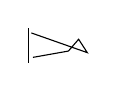
\begin{tikzpicture}
\draw (0,-.22)--(0,.22);
\draw (.04,.16)--(.75,-.09)--(.64,.08)--(.51,-.07)--(.06,-.15);
\end{tikzpicture}}}}

% 492-03: display (50).
\[
(50)\qquad \LMsourceMark{M000037}{\unsure{\widetilde{\mathcal T}_{1,1}}}
\longrightarrow \mathrm{GL}(2,\widehat{\mathbb Z})
\]

% 492-04: middle and lower paragraph.
et il faudrait \var{\deleted{\LMsourceMark{M000038}{\unsure{pouvoir}}}}{\LMsourceMark{M000039}{\LMcancelledDoubts{\LMsourceMark{M000040}{\unsure{pouvoir}}}}}{deletion}{140-3-s492-D004} interpréter cet homomorphisme
comme l'homomorphisme fondamental ``modulaire'' de la théorie des courbes
elliptiques (que l'image inverse de \var{\deleted{$\LMsourceMark{M000041}{\unsure{\Gamma}}$}}{\LMsourceMark{M000042}{\LMcancelledDoubts{\(\LMsourceMark{M000043}{\unsure{\Gamma}}\)}}}{deletion}{140-3-s492-D005}
$\Gamma_{\mathbb Q}\subset\widetilde\Gamma_{\mathbb Q}$ dans
$\LMsourceMark{M000044}{\unsure{\widetilde{\mathcal T}_{1,1}}}$ \LMsourceMark{M000045}{\unsure{puisse}} s'interpréter comme
$\LMsourceMark{M000046}{\unsure{\mathcal T_{1,1}}}\simeq\pi_1(M_{1,1\,\mathbb Q})$
doit être plus ou moins tautologique, par construction.)

% 492-05: final paragraph, interlinear addition, and display (51).
Il est clair en tous cas que les deux coïncident
\var{\inserted{pour tt $\gamma\in\widetilde M_{0,3}$}}{\LMadded{pour tt $\gamma\in\widetilde M_{0,3}$}}{insertion}{140-3-s492-I002}
\LMsourceMark{M000047}{\unsure{vus}} \LMsourceMark{M000048}{\unsure{comme|quand}} éléments de
\[
(51)\qquad \mu_2(\widehat{\mathbb Z})=\{\pm1\}^{\mathbb P}
\qquad (\mathbb P=\text{ens. des nbs. premiers})
\]
\LMsourceMark{M000049}{\mspage{491}}

\LMflushnotes\LMflushpages
\ifnum\LMform=1
\begin{LMapparatus}
\LMentry{140-3-s492-D001}{suppression}{\deleted{$\LMsourceMark{M000050}{\unsure{\Psi_{-\mathrm j}^{\pi}}}$}
}{\emph{\LMomittedlabel}}{Passage biffé dans le manuscrit : la suppression suit l'état final de l'auteur; les doutes de lecture restent signalés.}{}
\LMentry{140-3-s492-D002}{suppression}{\deleted{\LMsourceMark{M000051}{\unsure{par}} \LMsourceMark{M000052}{\illegible{2}}}
}{\emph{\LMomittedlabel}}{Passage biffé dans le manuscrit : la suppression suit l'état final de l'auteur; les doutes de lecture restent signalés.}{}
\LMentry{140-3-s492-D003}{suppression}{\deleted{\LMsourceMark{M000053}{\unsure{revêtement|profinie}} \LMsourceMark{M000054}{\unsure{à|de}} $\LMsourceMark{M000055}{\unsure{2}}$ \LMsourceMark{M000056}{\unsure{feuillets}}}
}{\emph{\LMomittedlabel}}{Passage biffé dans le manuscrit : la suppression suit l'état final de l'auteur; les doutes de lecture restent signalés.}{}
\LMentry{140-3-s492-I001}{insertion}{\inserted{extension ad-hoc}
}{\emph{\LMinsertedlabel}}{Ajout explicite de l'auteur : intégré à l'endroit indiqué par la transcription, sans modifier sa lecture.}{}
\LMentry{140-3-s492-D004}{suppression}{\deleted{\LMsourceMark{M000057}{\unsure{pouvoir}}}
}{\emph{\LMomittedlabel}}{Passage biffé dans le manuscrit : la suppression suit l'état final de l'auteur; les doutes de lecture restent signalés.}{}
\LMentry{140-3-s492-D005}{suppression}{\deleted{$\LMsourceMark{M000058}{\unsure{\Gamma}}$}
}{\emph{\LMomittedlabel}}{Passage biffé dans le manuscrit : la suppression suit l'état final de l'auteur; les doutes de lecture restent signalés.}{}
\LMentry{140-3-s492-I002}{insertion}{\inserted{pour tt $\gamma\in\widetilde M_{0,3}$}
}{\emph{\LMinsertedlabel}}{Ajout explicite de l'auteur : intégré à l'endroit indiqué par la transcription, sans modifier sa lecture.}{}
\end{LMapparatus}
\fi
\ifnum\LMform=2
\par\smallskip\begingroup\footnotesize\noindent\textcolor{gray}{\rule{.2\linewidth}{.35pt}}\par
\noindent\textit{\LMdoubtheading.}\par
\LMcarryover{140-3-s492-D001}{\(\LMsourceMark{M000059}{\unsure{\Psi_{-\mathrm j}^{\pi}}}\)
}
\LMcarryover{140-3-s492-D002}{\LMsourceMark{M000060}{\unsure{par}}\quad \LMsourceMark{M000061}{\illegible{2}}
}
\LMcarryover{140-3-s492-D003}{\LMsourceMark{M000062}{\unsure{revêtement|profinie}}\quad \LMsourceMark{M000063}{\unsure{à|de}}\quad \(\LMsourceMark{M000064}{\unsure{2}}\)\quad \LMsourceMark{M000065}{\unsure{feuillets}}
}
\LMcarryover{140-3-s492-D004}{\LMsourceMark{M000066}{\unsure{pouvoir}}
}
\LMcarryover{140-3-s492-D005}{\(\LMsourceMark{M000067}{\unsure{\Gamma}}\)
}
\par\endgroup\smallskip
\fi

\LMsourceMark{M000068}{\scanpage{493}}
\LMsourceMark{M000069}{\mspage{549}}
% 493-01: continuation, with an overwritten source in the first display.
i.e. ils coïncident modulo un hom
\[
\var{\deleted{\LMsourceMark{M000070}{\unsure{M_{0,3}}}}}{\LMsourceMark{M000071}{\LMcancelledDoubts{\(\LMsourceMark{M000072}{\unsure{M_{0,3}}}\)}}}{deletion}{140-3-s493-D001}\var{\inserted{\LMsourceMark{M000073}{\unsure{\widetilde\Gamma_{\mathbb Q}}}}}{\LMadded{\LMsourceMark{M000074}{\unsure{\widetilde\Gamma_{\mathbb Q}}}}}{insertion}{140-3-s493-I001}
\longrightarrow\mu_2(\widehat{\mathbb Z})\simeq\{\pm1\}^{\mathbb P}
\]
i.e. un hom
\[
\begin{aligned}
G_{\mathrm m}(\widehat{\mathbb Z})_2
&=(\widehat{\mathbb Z}^{*})_2\simeq\{\pm1\}^{\mathbb P}
\longrightarrow\var{\deleted{\LMsourceMark{M000075}{\unsure{\mu}}}}{\LMsourceMark{M000076}{\LMcancelledDoubts{\(\LMsourceMark{M000077}{\unsure{\mu}}\)}}}{deletion}{140-3-s493-D002}\LMsourceMark{M000078}{\unsure{{}_2G_{\mathrm m}}}(\widehat{\mathbb Z})
=\mu_2(\widehat{\mathbb Z})\\
&\hspace{24em}\simeq\{\pm1\}^{\mathbb P}
\end{aligned}
\]

% 493-02: middle prose.
--- donc ce n'est pas une \LMsourceMark{M000079}{\unsure{certaine}} ind. qui est en cause !
C'est moralement sûr que les deux coïncident --- je n'ai pas essayé de le
prouver.

% 493-03: lower prose and its interlinear insertion.
Quant à (35) (36), ils doivent correspondre sûrement à l'action de
$\Gamma_{\mathbb Q}$ sur les modules de Tate des courbes elliptiques à
isomorphismes exceptionnels, correspondant justement aux pts
$(1/2,2,-1)$ et $(-\overline{\mathrm j},-\mathrm j)$ de
$M_{0,3\,\mathbb Q}=M_{1,1}[2]'_{\mathbb Q}$.
L'indétermination de signe \var{\inserted{\LMsourceMark{M000080}{\unsure{doit|dont}}}}{\LMadded{\LMsourceMark{M000081}{\unsure{doit|dont}}}}{insertion}{140-3-s493-I002} \LMsourceMark{M000082}{\unsure{correspondre|correspond}} à l'indétermination
à remonter un point de $M_{1,1}[2]'_{\mathbb Q}$ en un point de
$M_{1,1}[2]_{\mathbb Q}$, i.e. de choisir une courbe elliptique
(avec ``\uline{rigidification}'' d'échelon 2) correspondant aux données de
\uline{Legendre} $(0,1,\infty,\LMsourceMark{M000083}{\unsure{q|\rho}})$ avec
$\LMsourceMark{M000084}{\unsure{\rho|q}}=1/2$ ou $\LMsourceMark{M000085}{\unsure{\rho|q}}=-\overline{\mathrm j}$.
\LMsourceMark{M000086}{\mspage{492}}

\LMflushnotes\LMflushpages
\ifnum\LMform=1
\begin{LMapparatus}
\LMentry{140-3-s493-D001}{suppression}{\(\deleted{\LMsourceMark{M000087}{\unsure{M_{0,3}}}}\)
}{\emph{\LMomittedlabel}}{Passage biffé dans le manuscrit : la suppression suit l'état final de l'auteur; les doutes de lecture restent signalés.}{}
\LMentry{140-3-s493-I001}{insertion}{\(\inserted{\LMsourceMark{M000088}{\unsure{\widetilde\Gamma_{\mathbb Q}}}}\)
}{\emph{\LMinsertedlabel}}{Ajout explicite de l'auteur : intégré à l'endroit indiqué par la transcription, sans modifier sa lecture.}{}
\LMentry{140-3-s493-D002}{suppression}{\(\deleted{\LMsourceMark{M000089}{\unsure{\mu}}}\)
}{\emph{\LMomittedlabel}}{Passage biffé dans le manuscrit : la suppression suit l'état final de l'auteur; les doutes de lecture restent signalés.}{}
\LMentry{140-3-s493-I002}{insertion}{\inserted{\LMsourceMark{M000090}{\unsure{doit|dont}}}
}{\emph{\LMinsertedlabel}}{Ajout explicite de l'auteur : intégré à l'endroit indiqué par la transcription, sans modifier sa lecture.}{}
\end{LMapparatus}
\fi
\ifnum\LMform=2
\par\smallskip\begingroup\footnotesize\noindent\textcolor{gray}{\rule{.2\linewidth}{.35pt}}\par
\noindent\textit{\LMdoubtheading.}\par
\LMcarryover{140-3-s493-D001}{\(\LMsourceMark{M000091}{\unsure{M_{0,3}}}\)
}
\LMcarryover{140-3-s493-D002}{\(\LMsourceMark{M000092}{\unsure{\mu}}\)
}
\par\endgroup\smallskip
\fi

\LMsourceMark{M000093}{\scanpage{494}}
% 494-01: upper paragraph.
Même une fois que l'\LMsourceMark{M000094}{\unsure{ambiguité}} de signe pour
$\Theta_{\LMsourceMark{M000095}{\unsure{G}}}^{\LMsourceMark{M000096}{\unsure{\pi}}}$ est levée en passant à l'extension
$\LMsourceMark{M000097}{\unsure{\widetilde{\mathcal T}_{1,1}}}$ à deux feuillets de
$\widetilde M_{0,3}$, l'indétermination des signes pour
$\Theta_{\rho}^{\LMsourceMark{M000098}{\unsure{\pi}}},\Theta_{\sigma}^{\LMsourceMark{M000099}{\unsure{\pi}}}$
n'est pas \LMsourceMark{M000100}{\unsure{levée}} pour autant, car les scindages
\var{\deleted{$\LMsourceMark{M000101}{\unsure{\Psi_{\rho}^{\pi},\Psi_{\sigma}^{\pi}}}$}}{\LMsourceMark{M000102}{\LMcancelledDoubts{\(\LMsourceMark{M000103}{\unsure{\Psi_{\rho}^{\pi},\Psi_{\sigma}^{\pi}}}\)}}}{deletion}{140-3-s494-D001}
$\Psi_{1/2}^{\LMsourceMark{M000104}{\unsure{\pi}}},\Psi_{-\overline{\mathrm j}}^{\LMsourceMark{M000105}{\unsure{\pi}}}$)
ne sont pas pour autant des scindages ($\overline{\mathrm m}$ partiels !)
de \var{\deleted{\LMsourceMark{M000106}{\unsure{cette}}}}{\LMsourceMark{M000107}{\LMcancelledDoubts{\LMsourceMark{M000108}{\unsure{cette}}}}}{deletion}{140-3-s494-D002} \LMsourceMark{M000109}{\unsure{l'extension}}
$\LMsourceMark{M000110}{\unsure{\widetilde{\mathcal T}_{1,1}}}$, mais seulement de
$\widetilde M_{0,3}$ --- et les remonter en des scindages de
$\LMsourceMark{M000111}{\unsure{\widetilde{\mathcal T}_{1,1}}}$
\var{\inserted{sur $\LMsourceMark{M000112}{\unsure{\mathcal T_{1,1}}}$,}}{\LMadded{sur $\LMsourceMark{M000113}{\unsure{\mathcal T_{1,1}}}$,}}{insertion}{140-3-s494-I001}
revient, très précisément, à choisir justement des courbes elliptiques à
rigidification de Legendre au dessus des pts $1/2,-\overline{\mathrm j}$.
Ainsi, des calculs faits en termes d'autom. des groupes à lacets
$\widehat\Pi_{0,3}$ \LMsourceMark{M000114}{\unsure{ou}} \var{\inserted{de}}{\LMadded{de}}{insertion}{140-3-s494-I002}
$\LMsourceMark{M000115}{\unsure{\mathcal{C}}}_{0,3}^{+\wedge}$,
\LMsourceMark{M000116}{\unsure{redonnent}} \var{\inserted{(sans les avoir \LMsourceMark{M000117}{\unsure{cherchés}} !)}}{\LMadded{(sans les avoir \LMsourceMark{M000118}{\unsure{cherchés}} !)}}{insertion}{140-3-s494-I003}
des résultats qui collent de très près à des vérités arithmético-géométriques
particulièrement cruciales.
\LMsourceMark{M000119}{\mspage{493}}

\Needspace{6\baselineskip}

\LMflushnotes\LMflushpages
\ifnum\LMform=1
\begin{LMapparatus}
\LMentry{140-3-s494-D001}{suppression}{\deleted{$\LMsourceMark{M000120}{\unsure{\Psi_{\rho}^{\pi},\Psi_{\sigma}^{\pi}}}$}
}{\emph{\LMomittedlabel}}{Passage biffé dans le manuscrit : la suppression suit l'état final de l'auteur; les doutes de lecture restent signalés.}{}
\LMentry{140-3-s494-D002}{suppression}{\deleted{\LMsourceMark{M000121}{\unsure{cette}}}
}{\emph{\LMomittedlabel}}{Passage biffé dans le manuscrit : la suppression suit l'état final de l'auteur; les doutes de lecture restent signalés.}{}
\LMentry{140-3-s494-I001}{insertion}{\inserted{sur $\LMsourceMark{M000122}{\unsure{\mathcal T_{1,1}}}$,}
}{\emph{\LMinsertedlabel}}{Ajout explicite de l'auteur : intégré à l'endroit indiqué par la transcription, sans modifier sa lecture.}{}
\LMentry{140-3-s494-I002}{insertion}{\inserted{de}
}{\emph{\LMinsertedlabel}}{Ajout explicite de l'auteur : intégré à l'endroit indiqué par la transcription, sans modifier sa lecture.}{}
\LMentry{140-3-s494-I003}{insertion}{\inserted{(sans les avoir \LMsourceMark{M000123}{\unsure{cherchés}} !)}
}{\emph{\LMinsertedlabel}}{Ajout explicite de l'auteur : intégré à l'endroit indiqué par la transcription, sans modifier sa lecture.}{}
\end{LMapparatus}
\fi
\ifnum\LMform=2
\par\smallskip\begingroup\footnotesize\noindent\textcolor{gray}{\rule{.2\linewidth}{.35pt}}\par
\noindent\textit{\LMdoubtheading.}\par
\LMcarryover{140-3-s494-D001}{\(\LMsourceMark{M000124}{\unsure{\Psi_{\rho}^{\pi},\Psi_{\sigma}^{\pi}}}\)
}
\LMcarryover{140-3-s494-D002}{\LMsourceMark{M000125}{\unsure{cette}}
}
\par\endgroup\smallskip
\fi

\LMsourceMark{M000126}{\scanpage{495}}
\LMsourceMark{M000127}{\mspage{550}}
% 495-01: heading.
49.\quad \uline{Homomorphismes de} $M_{0,3}$, les groupes
$M_{\rho,\sigma}$ généraux.

% 495-02: left-margin notes.
\LMsourceMark{M000128}{\margin{\LMsourceMark{M000129}{\unsure{Où on se met dans le bain}}\ldots}}
\LMsourceMark{M000130}{\margin{\LMsourceMark{M000131}{\unsure{Toute}} cette section \var{\inserted{I}}{\LMadded{I}}{insertion}{140-3-s495-I001} \LMsourceMark{M000132}{\unsure{semble}}
entièrement inutile pour la suite, c'est un \LMsourceMark{M000133}{\unsure{tâtonnement}}
préliminaire pour déboucher sur la section \uline{II} p.553.}}

% 495-03: first paragraph.
I) Considérons un sous-groupe \var{\inserted{fermé}}{\LMadded{fermé}}{insertion}{140-3-s495-I002} $G$ de $M_{0,3}$,
contenant $\LMsourceMark{M000134}{\unsure{\mathcal C}}_{0,3}^{+\wedge}$, donc image inverse d'un
sous-groupe fermé de $\widetilde\Gamma_{0,3}$.
On suppose que celui-ci est ``suffisamment gros'' --- disons qu'il contienne
un sous-groupe d'indice fini de
$\Gamma_{\mathbb Q}\subset\widetilde\Gamma_{0,3}$.
Pour le moment, on suppose pour simplifier que $G\subset\operatorname{Ker}\varepsilon_3$.
En résumé
\[
(1)\qquad
\LMsourceMark{M000135}{\unsure{\mathcal C}}_{0,3}^{+\wedge}\subset G\subset\widetilde M_{0,3},
\qquad u\in G\Longrightarrow\mu(u)\equiv1\ (3).
\]

% 495-04: interlinear correction and parallel maps.
Cette dernière hypothèse \var{\deleted{implique}}{}{deletion}{140-3-s495-D001}\var{\inserted{signifie}}{\LMadded{signifie}}{insertion}{140-3-s495-I003} donc que
pour tout $u\in G$, on a $\alpha_0(u)\in\LMsourceMark{M000136}{\unsure{\mathcal C}}_{0,3}^{\wedge+}$,
donc on a
\[
(\LMsourceMark{M000137}{\unsure{2}})\qquad
\diagram{\begin{tikzcd}[ampersand replacement=\&,column sep=large]
G \arrow[r,shift left=.7ex,"\underline{\alpha}_0"]
  \arrow[r,shift right=.7ex,"\underline{\beta}_0"']
\& \LMsourceMark{M000138}{\unsure{\mathcal C}}_{0,3}^{+}
\end{tikzcd}},
\]
caractérisées par
\[
(2')\qquad
\left\{\begin{aligned}
u(\rho)&=\operatorname{int}(\alpha_0)\rho\\
u(\sigma)&=\operatorname{int}(\beta_0)\sigma
\end{aligned}\right.
\qquad
\begin{aligned}
\alpha_0&=\underline{\alpha}_0(u)\\
\beta_0&=\underline{\beta}_0(u).
\end{aligned}
\]

% 495-05: the vertically arranged subgroups, including the intervening sign.
On considère
\[
(3)\qquad
\begin{array}{l}
G(0)=G\cap\widetilde M_{0,3}(0)\\[-.4em]
\quad\cap\\[-.4em]
G[0]=G\cap\widetilde M_{0,3}[0]=\operatorname{Norm}_{G}(L_0^{\LMsourceMark{M000139}{\unsure{\mathcal C}}})
\end{array}
\]
de sorte que
\[
\begin{aligned}
(4)\qquad&G=G(0).\LMsourceMark{M000140}{\unsure{\mathcal C}}_{0,3}^{+\wedge}
&&\text{(produit semi-direct)}\\
(5)\qquad&G[0]=G(0).L_0^{\LMsourceMark{M000141}{\unsure{\mathcal C}}}
&&\text{id}\\
(6)\qquad&G[0]\cap\LMsourceMark{M000142}{\unsure{\mathcal C}}_{0,3}^{+\wedge}
=L_0^{\LMsourceMark{M000143}{\unsure{\mathcal C}}}.
\end{aligned}
\]

% 495-06: definition (7) and last line.
On a posé
\[
(7)\qquad
\begin{gathered}
L_0^{\LMsourceMark{M000144}{\unsure{\mathcal C}}}=\text{sous-groupe fermé de }
\LMsourceMark{M000145}{\unsure{\mathcal C}}_{0,3}^{+\wedge}\text{ engendré}\\
\text{par }\varepsilon_0
\end{gathered}
\]
et on définit de $\overline{\mathrm m}$ $L_1^{\LMsourceMark{M000146}{\unsure{\mathcal C}}},L_{\infty}^{\LMsourceMark{M000147}{\unsure{\mathcal C}}}$.
\LMsourceMark{M000148}{\mspage{494}}

\LMflushnotes\LMflushpages
\ifnum\LMform=1
\begin{LMapparatus}
\LMentry{140-3-s495-I001}{insertion}{\inserted{I}
}{\emph{\LMinsertedlabel}}{Ajout explicite de l'auteur : intégré à l'endroit indiqué par la transcription, sans modifier sa lecture.}{}
\LMentry{140-3-s495-I002}{insertion}{\inserted{fermé}
}{\emph{\LMinsertedlabel}}{Ajout explicite de l'auteur : intégré à l'endroit indiqué par la transcription, sans modifier sa lecture.}{}
\LMentry{140-3-s495-D001}{suppression}{\deleted{implique}
}{\emph{\LMomittedlabel}}{Passage biffé dans le manuscrit : la suppression suit l'état final de l'auteur; les doutes de lecture restent signalés.}{}
\LMentry{140-3-s495-I003}{insertion}{\inserted{signifie}
}{\emph{\LMinsertedlabel}}{Ajout explicite de l'auteur : intégré à l'endroit indiqué par la transcription, sans modifier sa lecture.}{}
\end{LMapparatus}
\fi

\LMsourceMark{M000149}{\scanpage{496}}
% 496-01: paragraph and first map, with changes of target notation.
Considérons un groupe \var{\inserted{profini}}{\LMadded{profini}}{insertion}{140-3-s496-I001}
$\var{\deleted{\LMsourceMark{M000150}{\unsure{A}}}}{\LMsourceMark{M000151}{\LMcancelledDoubts{\(\LMsourceMark{M000152}{\unsure{A}}\)}}}{deletion}{140-3-s496-D001}\var{\inserted{M}}{\LMadded{M}}{insertion}{140-3-s496-I002}$, et un hom \var{\inserted{(continu)}}{\LMadded{(continu)}}{insertion}{140-3-s496-I003}
\uline{surjectif}
\[
(8)\qquad \varphi:G\longrightarrow\var{\deleted{\LMsourceMark{M000153}{\unsure{A}}}}{\LMsourceMark{M000154}{\LMcancelledDoubts{\(\LMsourceMark{M000155}{\unsure{A}}\)}}}{deletion}{140-3-s496-D002}M.
\]
On pose
\[
(9)\quad
\left\{\begin{aligned}
\varphi(\LMsourceMark{M000156}{\unsure{\mathcal C}}_{0,3}^{+\wedge})
 &=\LMsourceMark{M000157}{\unsure{\mathcal C}}\qquad\text{ss-groupe distingué de }M\\
\varphi(G(0))&=\var{\deleted{\LMsourceMark{M000158}{\unsure{A}}}}{\LMsourceMark{M000159}{\LMcancelledDoubts{\(\LMsourceMark{M000160}{\unsure{A}}\)}}}{deletion}{140-3-s496-D003}\var{\inserted{M}}{\LMadded{M}}{insertion}{140-3-s496-I004}(0)\\
\varphi(G[0])&=\var{\deleted{\LMsourceMark{M000161}{\unsure{A}}}}{\LMsourceMark{M000162}{\LMcancelledDoubts{\(\LMsourceMark{M000163}{\unsure{A}}\)}}}{deletion}{140-3-s496-D004}\var{\inserted{M}}{\LMadded{M}}{insertion}{140-3-s496-I005}[0].\\
\varphi(L_0^{\LMsourceMark{M000164}{\unsure{\mathcal C}}})&=L_0^{\var{\deleted{\LMsourceMark{M000165}{\unsure{\mathcal C}}}}{\LMsourceMark{M000166}{\LMcancelledDoubts{\(\LMsourceMark{M000167}{\unsure{\mathcal C}}\)}}}{deletion}{140-3-s496-D005}}
\end{aligned}\right.
\]

% 496-02: subgroup relations.
\var{\deleted{\LMsourceMark{M000168}{\unsure{Donc}}}}{\LMsourceMark{M000169}{\LMcancelledDoubts{\LMsourceMark{M000170}{\unsure{Donc}}}}}{deletion}{140-3-s496-D006}

Donc ce sont des sous-groupes fermés de $M$, satisfaisant
\[
\begin{aligned}
(10)\qquad&M(0)\subset M[0]\subset\operatorname{Norm}_{M}(L_0)\\
(11)\qquad&L_0^{\var{\deleted{\LMsourceMark{M000171}{\unsure{\mathcal C}}}}{\LMsourceMark{M000172}{\LMcancelledDoubts{\(\LMsourceMark{M000173}{\unsure{\mathcal C}}\)}}}{deletion}{140-3-s496-D007}}
\subset\LMsourceMark{M000174}{\unsure{\mathcal C}}\cap M[0].
\end{aligned}
\]

% 496-03: the surviving generator relations.
Par abus de langage, on désigne encore par $\rho,\sigma,\varepsilon_0,\varepsilon_1$
\ldots\ les images de ces éléments dans $\LMsourceMark{M000175}{\unsure{\mathcal C}}$, qui y
satisfont donc les relations connues dans $\LMsourceMark{M000176}{\unsure{\mathcal C}}_{0,3}^{+\wedge}$,
en particulier
\[
(12)\qquad
\sigma^2=\rho^3=1,\qquad
\sigma\rho=\varepsilon_0,\quad \rho\sigma=\varepsilon_1,\qquad
\varepsilon_1=\sigma(\varepsilon_0)=\rho(\varepsilon_0).
\]

% 496-04: paragraph and revised definition (13).
Les restrictions des applications $\alpha_0,\beta_0$ de (2,2') à
$M_{\rho,\sigma}[0]$ seront plutôt notées $\alpha,\beta$, où $\alpha,\beta$
sont en fait des applications
\[
(13)\quad
\diagram{\begin{tikzcd}[ampersand replacement=\&,column sep=large]
{\begin{gathered}
SG\overset{\mathrm{dfn}}=\var{\deleted{\text{extension de}}}{}{deletion}{140-3-s496-D008}\ G\\
\text{par }L_0^{\LMsourceMark{M000177}{\unsure{\mathcal C}}},\ \text{image}\\
\text{inverse de }\LMsourceMark{M000178}{\unsure{G}}\\
\text{dans }S\widetilde M_{0,3}\\
=\{(u,f)\in G\times\LMsourceMark{M000179}{\unsure{\mathcal C}}_{0,3}^{+\wedge}\mid fu\in G[0]
\end{gathered}}
\arrow[r,shift left=.7ex,"\alpha"]
\arrow[r,shift right=.7ex,"\beta"']
\&\LMsourceMark{M000180}{\unsure{\mathcal C}}_{0,3}^{+\wedge}
\end{tikzcd}}
\]
dont on regarde les restrictions au \uline{sous-groupe}
($\simeq M_{\rho,\sigma}[0]$) de $SG$ défini par la relation $f=1$.

% 496-05: composition of the two functions, and (14).
Composant $\underline\alpha,\underline\beta:$
\diagram{\begin{tikzcd}[ampersand replacement=\&,column sep=small]
\var{\deleted{\LMsourceMark{M000181}{\unsure{M[0]}}}}{\LMsourceMark{M000182}{\LMcancelledDoubts{\(\LMsourceMark{M000183}{\unsure{M[0]}}\)}}}{deletion}{140-3-s496-D009}\var{\inserted{G[0]}}{\LMadded{G[0]}}{insertion}{140-3-s496-I006}
\arrow[r,shift left=.5ex]\arrow[r,shift right=.5ex]
\&\LMsourceMark{M000184}{\unsure{\mathcal C}}_{0,3}^{+\wedge}
\end{tikzcd}}
avec $\varphi\mid\LMsourceMark{M000185}{\unsure{\mathcal C}}_{0,3}^{+\wedge}$, on trouve des
applications, encore notées $\underline\alpha,\underline\beta$
(où $\underline\alpha^M,\underline\beta^M$ en cas de confusion possible)
\[
(14)\qquad
\diagram{\begin{tikzcd}[ampersand replacement=\&,column sep=large]
G[0]\arrow[r,shift left=.7ex,"\underline\alpha"]
\arrow[r,shift right=.7ex,"\underline\beta"']
\&\LMsourceMark{M000186}{\unsure{\mathcal C}}
\end{tikzcd}}
\]
satisfaisant donc
\[
(15)\qquad
\left\{\begin{aligned}
\LMsourceMark{M000187}{\unsure{u}}(\rho)&=\operatorname{int}(\alpha)\rho\\
\LMsourceMark{M000188}{\unsure{u}}(\sigma)&=\operatorname{int}(\beta)\sigma
\end{aligned}\right.
\qquad
\begin{gathered}
\text{pour }u\in M[0]\ \var{\inserted{\text{\LMsourceMark{M000189}{\unsure{de}}}}}{\LMadded{\text{\LMsourceMark{M000190}{\unsure{de}}}}}{insertion}{140-3-s496-I007}\text{ la forme }\varphi(u_0),\\
\text{et }\alpha=\underline\alpha(u_0),\ \beta=\underline\beta(u_0).
\end{gathered}
\]
\LMsourceMark{M000191}{\mspage{495}}

\LMflushnotes\LMflushpages
\ifnum\LMform=1
\begin{LMapparatus}
\LMentry{140-3-s496-I001}{insertion}{\inserted{profini}
}{\emph{\LMinsertedlabel}}{Ajout explicite de l'auteur : intégré à l'endroit indiqué par la transcription, sans modifier sa lecture.}{}
\LMentry{140-3-s496-D001}{suppression}{\(\deleted{\LMsourceMark{M000192}{\unsure{A}}}\)
}{\emph{\LMomittedlabel}}{Passage biffé dans le manuscrit : la suppression suit l'état final de l'auteur; les doutes de lecture restent signalés.}{}
\LMentry{140-3-s496-I002}{insertion}{\(\inserted{M}\)
}{\emph{\LMinsertedlabel}}{Ajout explicite de l'auteur : intégré à l'endroit indiqué par la transcription, sans modifier sa lecture.}{}
\LMentry{140-3-s496-I003}{insertion}{\inserted{(continu)}
}{\emph{\LMinsertedlabel}}{Ajout explicite de l'auteur : intégré à l'endroit indiqué par la transcription, sans modifier sa lecture.}{}
\LMentry{140-3-s496-D002}{suppression}{\(\deleted{\LMsourceMark{M000193}{\unsure{A}}}\)
}{\emph{\LMomittedlabel}}{Passage biffé dans le manuscrit : la suppression suit l'état final de l'auteur; les doutes de lecture restent signalés.}{}
\LMentry{140-3-s496-D003}{suppression}{\(\deleted{\LMsourceMark{M000194}{\unsure{A}}}\)
}{\emph{\LMomittedlabel}}{Passage biffé dans le manuscrit : la suppression suit l'état final de l'auteur; les doutes de lecture restent signalés.}{}
\LMentry{140-3-s496-I004}{insertion}{\(\inserted{M}\)
}{\emph{\LMinsertedlabel}}{Ajout explicite de l'auteur : intégré à l'endroit indiqué par la transcription, sans modifier sa lecture.}{}
\LMentry{140-3-s496-D004}{suppression}{\(\deleted{\LMsourceMark{M000195}{\unsure{A}}}\)
}{\emph{\LMomittedlabel}}{Passage biffé dans le manuscrit : la suppression suit l'état final de l'auteur; les doutes de lecture restent signalés.}{}
\LMentry{140-3-s496-I005}{insertion}{\(\inserted{M}\)
}{\emph{\LMinsertedlabel}}{Ajout explicite de l'auteur : intégré à l'endroit indiqué par la transcription, sans modifier sa lecture.}{}
\LMentry{140-3-s496-D005}{suppression}{\(\deleted{\LMsourceMark{M000196}{\unsure{\mathcal C}}}\)
}{\emph{\LMomittedlabel}}{Passage biffé dans le manuscrit : la suppression suit l'état final de l'auteur; les doutes de lecture restent signalés.}{}
\LMentry{140-3-s496-D006}{suppression}{\deleted{\LMsourceMark{M000197}{\unsure{Donc}}}
}{\emph{\LMomittedlabel}}{Passage biffé dans le manuscrit : la suppression suit l'état final de l'auteur; les doutes de lecture restent signalés.}{}
\LMentry{140-3-s496-D007}{suppression}{\(\deleted{\LMsourceMark{M000198}{\unsure{\mathcal C}}}\)
}{\emph{\LMomittedlabel}}{Passage biffé dans le manuscrit : la suppression suit l'état final de l'auteur; les doutes de lecture restent signalés.}{}
\LMentry{140-3-s496-D008}{suppression}{\(\deleted{\text{extension de}}\)
}{\emph{\LMomittedlabel}}{Passage biffé dans le manuscrit : la suppression suit l'état final de l'auteur; les doutes de lecture restent signalés.}{}
\LMentry{140-3-s496-D009}{suppression}{\(\deleted{\LMsourceMark{M000199}{\unsure{M[0]}}}\)
}{\emph{\LMomittedlabel}}{Passage biffé dans le manuscrit : la suppression suit l'état final de l'auteur; les doutes de lecture restent signalés.}{}
\LMentry{140-3-s496-I006}{insertion}{\(\inserted{G[0]}\)
}{\emph{\LMinsertedlabel}}{Ajout explicite de l'auteur : intégré à l'endroit indiqué par la transcription, sans modifier sa lecture.}{}
\LMentry{140-3-s496-I007}{insertion}{\(\inserted{\text{\LMsourceMark{M000200}{\unsure{de}}}}\)
}{\emph{\LMinsertedlabel}}{Ajout explicite de l'auteur : intégré à l'endroit indiqué par la transcription, sans modifier sa lecture.}{}
\end{LMapparatus}
\fi
\ifnum\LMform=2
\par\smallskip\begingroup\footnotesize\noindent\textcolor{gray}{\rule{.2\linewidth}{.35pt}}\par
\noindent\textit{\LMdoubtheading.}\par
\LMcarryover{140-3-s496-D001}{\(\LMsourceMark{M000201}{\unsure{A}}\)
}
\LMcarryover{140-3-s496-D002}{\(\LMsourceMark{M000202}{\unsure{A}}\)
}
\LMcarryover{140-3-s496-D003}{\(\LMsourceMark{M000203}{\unsure{A}}\)
}
\LMcarryover{140-3-s496-D004}{\(\LMsourceMark{M000204}{\unsure{A}}\)
}
\LMcarryover{140-3-s496-D005}{\(\LMsourceMark{M000205}{\unsure{\mathcal C}}\)
}
\LMcarryover{140-3-s496-D006}{\LMsourceMark{M000206}{\unsure{Donc}}
}
\LMcarryover{140-3-s496-D007}{\(\LMsourceMark{M000207}{\unsure{\mathcal C}}\)
}
\LMcarryover{140-3-s496-D009}{\(\LMsourceMark{M000208}{\unsure{M[0]}}\)
}
\par\endgroup\smallskip
\fi

\LMsourceMark{M000209}{\scanpage{497}}
\LMsourceMark{M000210}{\mspage{551}}

% 497-01
A priori, $\alpha$ et $\beta$ dépendent du choix de $u_0$ dont $u$ provient
pas seulement de $u$ --- mais
% 497-02
\[
(16)\qquad
\left\{\begin{aligned}
\alpha\rho(\alpha)^{-1}&=[u,\rho]\\
\beta\sigma(\beta)^{-1}&=[u,\sigma]
\end{aligned}\right.
\]
% 497-03
n'en dépendent pas. Si on pose
% 497-04
\[
(17)\qquad
T_{\rho}=\uline{\mathrm{Centr}}_M(\rho)
\qquad
T_{\sigma}=\uline{\mathrm{Centr}}_M(\sigma)
\]
% 497-05
on voit donc que, modulo $T_{\rho}$ resp. $T_{\sigma}$,
$\alpha,\beta$ ne dépendent que de $u$.

% 497-06, 497-07, 497-08, 497-09
\uline{Hypothèse}
$\alpha\var{\inserted{{}=\alpha(u_0)}}{\LMadded{{}=\alpha(u_0)}}{insertion}{140-3-s497-I001},\beta\var{\inserted{{}=\beta(u_0)}}{\LMadded{{}=\beta(u_0)}}{insertion}{140-3-s497-I002}$
ne dépendent que de $u=\varphi(u_0)$
(pour $u_0\in\var{\deleted{\LMsourceMark{M000211}{\unsure{M}}}}{\LMsourceMark{M000212}{\LMcancelledDoubts{\(\LMsourceMark{M000213}{\unsure{M}}\)}}}{deletion}{140-3-s497-D001}\LMsourceMark{M000214}{\unsure{G}}[0]$).

% 497-10
On va \LMsourceMark{M000215}{\unsure{exprimer}} cette hypothèse de façon un peu différente,
en introduisant
% 497-11
\[
(18)\qquad J=\operatorname{Ker}(G[0]\longrightarrow M[0]),
\]
% 497-12, 497-13
on veut donc que pour $\var{\deleted{\LMsourceMark{M000216}{\unsure{\alpha}}}}{\LMsourceMark{M000217}{\LMcancelledDoubts{\(\LMsourceMark{M000218}{\unsure{\alpha}}\)}}}{deletion}{140-3-s497-D002}$
% 497-14, 497-15
\[
u'_0=\var{\deleted{u_0}}{}{deletion}{140-3-s497-D003}\delta_0u_0\quad
\text{avec }u_0\in G[0],\ \delta_0\in J,\quad\text{on ait}
\]
% 497-16
\[
\alpha(u'_0)=\alpha(u_0),\qquad \beta(u'_0)=\beta(u_0)
\]
% 497-17, 497-18
\LMsourceMark{M000219}{\unsure{Notons}}
\[
\begin{gathered}
\alpha_0=\uline{\alpha}(u_0),\quad
\beta_0=\uline{\beta}(u_0),\quad
\alpha'_0=\uline{\alpha}(u'_0),\quad
\beta'_0=\uline{\beta}(u'_0),\quad
\overline{\alpha}_0=\uline{\alpha}(\delta_0),\quad
\overline{\beta}_0=\uline{\beta}(\LMsourceMark{M000220}{\unsure{\delta_1|\delta_0}}),
\end{gathered}
\]
\uline{dans} $G$, de sorte qu'on aura, par les formules de cocycles de $G$
% 497-19
\[
\alpha'_0=\delta_0(\alpha_0)\overline{\alpha}_0,
\qquad
\beta'_0=\delta_0(\beta_0)\overline{\beta}_0,
\]
% 497-20
d'où, en appliquant $\varphi$ et notant que
% 497-21
\[
\begin{aligned}
\varphi(\delta_0(\alpha_0))
&=\underbrace{\varphi(\delta_0)}_{1}(\varphi(\alpha_0))
=\varphi(\alpha_0)\overset{\mathrm{dfn}}=\alpha
&&\text{et de }\overline{\mathrm m}\\
\varphi(\delta_0(\beta_0))&=\varphi(\beta_0)\overset{\mathrm{dfn}}=\beta
\end{aligned}
\]
% 497-22, 497-23
\[
(19)\qquad
\alpha'=\var{\deleted{\LMsourceMark{M000221}{\unsure{\varphi}}}}{\LMsourceMark{M000222}{\LMcancelledDoubts{\(\LMsourceMark{M000223}{\unsure{\varphi}}\)}}}{deletion}{140-3-s497-D004}\alpha\overline{\alpha},\qquad
\beta'=\beta\overline{\beta}\qquad\text{dans }\LMsourceMark{M000224}{\unsure{\mathcal{C}}}
\]
% 497-24, 497-25
où $\alpha,\beta,\alpha',\beta',\overline{\alpha},\overline{\beta}$ sont les images par
$\varphi$ des quantités $\alpha_0$ etc dans $\LMsourceMark{M000225}{\unsure{\mathcal{C}}}_{0,3}^{+\wedge}$.
\var{\deleted{\LMsourceMark{M000226}{\unsure{avec}} $\alpha=\alpha(u_0)$}}{\LMsourceMark{M000227}{\LMcancelledDoubts{\LMsourceMark{M000228}{\unsure{avec}}}}}{deletion}{140-3-s497-D005}
Donc l'hypothèse signifie ceci
% 497-26
\[
(20)\qquad
\forall\,\delta_0\in J\overset{\mathrm{dfn}}=
\operatorname{Ker}(G[0]\longrightarrow M[0]),\quad
\text{on a}\quad
\LMsourceMark{M000229}{\unsure{\alpha^{\Pi}}}(\delta_0),\LMsourceMark{M000230}{\unsure{\beta^{\Pi}}}(\delta_0)
\in\LMsourceMark{M000231}{\unsure{\operatorname{Ker}}}\varphi
\]
% 497-27, 497-28
\var{\deleted{\LMsourceMark{M000232}{\unsure{lorsque}}}}{\LMsourceMark{M000233}{\LMcancelledDoubts{\LMsourceMark{M000234}{\unsure{lorsque}}}}}{deletion}{140-3-s497-D006}
Quand cette hypothèse est satisfaite, on a donc des applications
\LMsourceMark{M000235}{\mspage{496}}

\LMflushnotes\LMflushpages
\ifnum\LMform=1
\begin{LMapparatus}
\LMentry{140-3-s497-I001}{insertion}{\(\inserted{{}=\alpha(u_0)}\)
}{\emph{\LMinsertedlabel}}{Ajout explicite de l'auteur : intégré à l'endroit indiqué par la transcription, sans modifier sa lecture.}{}
\LMentry{140-3-s497-I002}{insertion}{\(\inserted{{}=\beta(u_0)}\)
}{\emph{\LMinsertedlabel}}{Ajout explicite de l'auteur : intégré à l'endroit indiqué par la transcription, sans modifier sa lecture.}{}
\LMentry{140-3-s497-D001}{suppression}{\(\deleted{\LMsourceMark{M000236}{\unsure{M}}}\)
}{\emph{\LMomittedlabel}}{Passage biffé dans le manuscrit : la suppression suit l'état final de l'auteur; les doutes de lecture restent signalés.}{}
\LMentry{140-3-s497-D002}{suppression}{\(\deleted{\LMsourceMark{M000237}{\unsure{\alpha}}}\)
}{\emph{\LMomittedlabel}}{Passage biffé dans le manuscrit : la suppression suit l'état final de l'auteur; les doutes de lecture restent signalés.}{}
\LMentry{140-3-s497-D003}{suppression}{\(\deleted{u_0}\)
}{\emph{\LMomittedlabel}}{Passage biffé dans le manuscrit : la suppression suit l'état final de l'auteur; les doutes de lecture restent signalés.}{}
\LMentry{140-3-s497-D004}{suppression}{\(\deleted{\LMsourceMark{M000238}{\unsure{\varphi}}}\)
}{\emph{\LMomittedlabel}}{Passage biffé dans le manuscrit : la suppression suit l'état final de l'auteur; les doutes de lecture restent signalés.}{}
\LMentry{140-3-s497-D005}{suppression}{\deleted{\LMsourceMark{M000239}{\unsure{avec}} $\alpha=\alpha(u_0)$}
}{\emph{\LMomittedlabel}}{Passage biffé dans le manuscrit : la suppression suit l'état final de l'auteur; les doutes de lecture restent signalés.}{}
\LMentry{140-3-s497-D006}{suppression}{\deleted{\LMsourceMark{M000240}{\unsure{lorsque}}}
}{\emph{\LMomittedlabel}}{Passage biffé dans le manuscrit : la suppression suit l'état final de l'auteur; les doutes de lecture restent signalés.}{}
\end{LMapparatus}
\fi
\ifnum\LMform=2
\par\smallskip\begingroup\footnotesize\noindent\textcolor{gray}{\rule{.2\linewidth}{.35pt}}\par
\noindent\textit{\LMdoubtheading.}\par
\LMcarryover{140-3-s497-D001}{\(\LMsourceMark{M000241}{\unsure{M}}\)
}
\LMcarryover{140-3-s497-D002}{\(\LMsourceMark{M000242}{\unsure{\alpha}}\)
}
\LMcarryover{140-3-s497-D004}{\(\LMsourceMark{M000243}{\unsure{\varphi}}\)
}
\LMcarryover{140-3-s497-D005}{\LMsourceMark{M000244}{\unsure{avec}}
}
\LMcarryover{140-3-s497-D006}{\LMsourceMark{M000245}{\unsure{lorsque}}
}
\par\endgroup\smallskip
\fi

\LMsourceMark{M000246}{\scanpage{498}}

% 498-01
\[
(21)\qquad
\diagram{\begin{tikzcd}[ampersand replacement=\&,column sep=large]
M[0]\arrow[r,shift left=0.65ex,"\uline{\alpha}"]
\arrow[r,shift right=0.65ex,"\uline{\beta}"']\&\LMsourceMark{M000247}{\unsure{\mathcal{C}}}
\end{tikzcd}}
\]
% 498-02, 498-03
\var{\deleted{satisfaisant}}{}{deletion}{140-3-s498-D001}
\LMsourceMark{M000248}{\unsure{factorisant}} (14), et satisfaisant donc
% 498-04
\[
(22)\qquad
\left\{\begin{aligned}
u(\rho)&=\operatorname{int}(\alpha)\rho\\
\LMsourceMark{M000249}{\unsure{u}}(\sigma)&=\operatorname{int}(\beta)\sigma
\end{aligned}\right.
\qquad
\text{pour }\LMsourceMark{M000250}{\unsure{u}}\in M[0],\quad
\alpha=\uline{\alpha}(u),\quad\beta=\uline{\beta}(u),
\]
% 498-05, 498-06, 498-07
qui \var{\deleted{\LMsourceMark{M000251}{\unsure{généralisent|généralisant}}}}{\LMsourceMark{M000252}{\LMcancelledDoubts{\LMsourceMark{M000253}{\unsure{généralisent|généralisant}}}}}{deletion}{140-3-s498-D002}
\var{\inserted{\LMsourceMark{M000254}{\unsure{paraphrasent}}}}{\LMadded{\LMsourceMark{M000255}{\unsure{paraphrasent}}}}{insertion}{140-3-s498-I001} (2').

% 498-08
D'ailleurs, posons
% 498-09
\[
(23)\qquad
\LMsourceMark{M000256}{\unsure{\zeta|\xi}}=\alpha\rho(\alpha)^{-1},\qquad
\eta=\beta\sigma(\beta)^{-1}
\]
% 498-10
les relations (22) s'écrivent ainsi
% 498-11
\[
(24)\qquad u(\rho)=\LMsourceMark{M000257}{\unsure{\zeta|\xi}}\rho,\qquad u(\sigma)=\eta\sigma
\]
% 498-12
et on aura
% 498-13
\[
(25)\qquad \LMsourceMark{M000258}{\unsure{\zeta|\xi}}=[u,\rho],\qquad \eta=[u,\sigma]
\]
% 498-14
et de plus
% 498-15
\[
(26)\qquad
\LMsourceMark{M000259}{\unsure{\zeta|\xi}}=\eta\LMsourceMark{M000260}{\unsure{\varepsilon_1|\ell_1}}^{\nu}\qquad
\text{où }\nu=\frac{\mu-1}{2}\in\widehat{\mathbb Z}
\quad\text{($\mu$ le multiplicateur de $u$).}
\]
% 498-16
qui provient de la relation unique dans $\LMsourceMark{M000261}{\unsure{\mathcal{C}}}_{0,3}^{+}$.

% 498-17
(On suppose pour fixer les idées que l'hom
% 498-18, 498-19
\[
\var{\deleted{\LMsourceMark{M000262}{\unsure{(27)}}}}{\LMsourceMark{M000263}{\LMcancelledDoubts{\(\LMsourceMark{M000264}{\unsure{(27)}}\)}}}{deletion}{140-3-s498-D003}\qquad
\diagram{\begin{tikzcd}[ampersand replacement=\&,column sep=large]
G\arrow[r,"\chi^{G}"]\&\widehat{\mathbb Z}^{*}
\end{tikzcd}}
\qquad\text{(``multiplicateur'')}
\]
% 498-20
se factorise par
% 498-21
\[
(27)\qquad
\diagram{\begin{tikzcd}[ampersand replacement=\&,column sep=large]
G\arrow[r]\&M\arrow[r,"\chi^{M}"]\&\widehat{\mathbb Z}^{*},
\end{tikzcd}}
\]
% 498-22
de sorte qu'on a une notion de multiplicateur ($\in\widehat{\mathbb Z}^{*}$)
pour les $u\in M$.)

% 498-23
Considérons l'hom naturel
% 498-24
\[
(28)\qquad
\diagram{\begin{tikzcd}[ampersand replacement=\&,column sep=large,row sep=small]
M[0]\arrow[r]\&\operatorname{Aut}(\LMsourceMark{M000265}{\unsure{\mathcal{C}}}):\\
u\arrow[r,mapsto]\&\operatorname{int}(u)|\LMsourceMark{M000266}{\unsure{\mathcal{C}}}
\end{tikzcd}}
\]
% 498-25, 498-26
on voit sur (22) \var{\inserted{\LMsourceMark{M000267}{\unsure{même|ou $\overline{\mathrm m}$}} (24)}}{\LMadded{\LMsourceMark{M000268}{\unsure{même|ou $\overline{\mathrm m}$}} (24)}}{insertion}{140-3-s498-I002}
qu'il est connu quand on connaît
\LMsourceMark{M000269}{\mspage{497}}

\LMflushnotes\LMflushpages
\ifnum\LMform=1
\begin{LMapparatus}
\LMentry{140-3-s498-D001}{suppression}{\deleted{satisfaisant}
}{\emph{\LMomittedlabel}}{Passage biffé dans le manuscrit : la suppression suit l'état final de l'auteur; les doutes de lecture restent signalés.}{}
\LMentry{140-3-s498-D002}{suppression}{\deleted{\LMsourceMark{M000270}{\unsure{généralisent|généralisant}}}
}{\emph{\LMomittedlabel}}{Passage biffé dans le manuscrit : la suppression suit l'état final de l'auteur; les doutes de lecture restent signalés.}{}
\LMentry{140-3-s498-I001}{insertion}{\inserted{\LMsourceMark{M000271}{\unsure{paraphrasent}}}
}{\emph{\LMinsertedlabel}}{Ajout explicite de l'auteur : intégré à l'endroit indiqué par la transcription, sans modifier sa lecture.}{}
\LMentry{140-3-s498-D003}{suppression}{\(\deleted{\LMsourceMark{M000272}{\unsure{(27)}}}\)
}{\emph{\LMomittedlabel}}{Passage biffé dans le manuscrit : la suppression suit l'état final de l'auteur; les doutes de lecture restent signalés.}{}
\LMentry{140-3-s498-I002}{insertion}{\inserted{\LMsourceMark{M000273}{\unsure{même|ou $\overline{\mathrm m}$}} (24)}
}{\emph{\LMinsertedlabel}}{Ajout explicite de l'auteur : intégré à l'endroit indiqué par la transcription, sans modifier sa lecture.}{}
\end{LMapparatus}
\fi
\ifnum\LMform=2
\par\smallskip\begingroup\footnotesize\noindent\textcolor{gray}{\rule{.2\linewidth}{.35pt}}\par
\noindent\textit{\LMdoubtheading.}\par
\LMcarryover{140-3-s498-D002}{\LMsourceMark{M000274}{\unsure{généralisent|généralisant}}
}
\LMcarryover{140-3-s498-D003}{\(\LMsourceMark{M000275}{\unsure{(27)}}\)
}
\par\endgroup\smallskip
\fi

\LMsourceMark{M000276}{\scanpage{499}}
\LMsourceMark{M000277}{\mspage{552}}

% 499-01, 499-02
\LMsourceMark{M000278}{\margin{car \var{\deleted{\LMsourceMark{M000279}{\illegible{1}}}}{\LMsourceMark{M000280}{\LMcancelledDoubts{\LMsourceMark{M000281}{\illegible{1}}}}}{deletion}{140-3-s499-D001} $\rho,\sigma$ engendrent
\LMsourceMark{M000282}{\unsure{topolog$^t$}} $\LMsourceMark{M000283}{\unsure{\mathcal{C}}}$}}
% 499-03
les fonctions $\uline{\alpha},\uline{\beta}:M[0]\longrightarrow\LMsourceMark{M000284}{\unsure{\mathcal{C}}}$,
et $\overline{\mathrm m}$ quand on connaît seulement
$\LMsourceMark{M000285}{\unsure{\zeta|\xi}},\eta:M[0]\longrightarrow\LMsourceMark{M000286}{\unsure{\mathcal{C}}}$.
Si d'ailleurs on pose
% 499-04
\[
(29)\qquad
M'[0]=\operatorname{Im}(M[0]\longrightarrow\operatorname{Aut}(\LMsourceMark{M000287}{\unsure{\mathcal{C}}}))
\]
% 499-05
ces dernières fonctions $\LMsourceMark{M000288}{\unsure{\zeta|\xi}},\eta$ sont déjà définies sur $M'[0]$ --- alors qu'il
n'est pas clair qu'il en soit de $\overline{\mathrm m}$ de $\alpha,\beta$, quand
$M[0]$ \LMsourceMark{M000289}{\unsure{n'agit|n'opère}} pas fidèlement sur $\LMsourceMark{M000290}{\unsure{\mathcal{C}}}$.
On a ainsi une application \var{\inserted{$(\LMsourceMark{M000291}{\unsure{\zeta|\xi}},\eta)$}}{\LMadded{$(\LMsourceMark{M000292}{\unsure{\zeta|\xi}},\eta)$}}{insertion}{140-3-s499-I001} d'un certain sous-groupe
$M'[0]\subset\operatorname{Norm}_{\operatorname{Aut}(\LMsourceMark{M000293}{\unsure{\mathcal{C}}})}(L_0)$
dans l'ens $\LMsourceMark{M000294}{\unsure{\mathcal{R}}}$ des solutions de l'équation en $\LMsourceMark{M000295}{\unsure{\zeta|\xi}},\eta$
(26) qu'on \LMsourceMark{M000296}{\unsure{écrit|écrira}} simplement
% 499-06
\[
(30)\qquad \eta^{-1}\LMsourceMark{M000297}{\unsure{\zeta|\xi}}\in L_1
\]
% 499-07, 499-08
relation qui implique (26) (avec la forme précise de l'exposant $\nu$)
si on suppose \var{\inserted{(\LMsourceMark{M000298}{\unsure{p.ex.}})}}{\LMadded{(\LMsourceMark{M000299}{\unsure{p.ex.}})}}{insertion}{140-3-s499-I002} $\LMsourceMark{M000300}{\unsure{\mathcal{C}|M}}$ assez gros pour que
% 499-09
\var{\inserted{$\diagram{\begin{tikzcd}[ampersand replacement=\&,column sep=large]
\LMsourceMark{M000301}{\unsure{\mathcal{C}}}_{0,3}^{+\wedge}\arrow[r,"\LMsourceMark{M000302}{\unsure{2}}"']\&
\LMsourceMark{M000303}{\unsure{\mathrm{SL}|\mathrm{PSL}}}(2,\widehat{\mathbb Z})
\end{tikzcd}}$}}{\LMadded{$\diagram{\begin{tikzcd}[ampersand replacement=\&,column sep=large]
\LMsourceMark{M000304}{\unsure{\mathcal{C}}}_{0,3}^{+\wedge}\arrow[r,"\LMsourceMark{M000305}{\unsure{2}}"']\&
\LMsourceMark{M000306}{\unsure{\mathrm{SL}|\mathrm{PSL}}}(2,\widehat{\mathbb Z})
\end{tikzcd}}$}}{insertion}{140-3-s499-I003}
se factorise par $\LMsourceMark{M000307}{\unsure{\mathcal{C}}}$ --- ce qu'on va supposer, pour nous simplifier la vie.

% 499-10, 499-11
\var{\deleted{On va faire sur $\LMsourceMark{M000308}{\unsure{\mathcal{C}}}$, muni de $\rho,\sigma,\varepsilon_1$
l'hypothèse suivante}}{\LMsourceMark{M000309}{\LMcancelledDoubts{\(\LMsourceMark{M000310}{\unsure{\mathcal{C}}}\)}}}{deletion}{140-3-s499-D002}
\var{\inserted{De façon plus précise, soit}}{\LMadded{De façon plus précise, soit}}{insertion}{140-3-s499-I004}
% 499-12
\var{\deleted{(31) \LMsourceMark{M000311}{\unsure{H)|II)}} Sur}}{\LMsourceMark{M000312}{\LMcancelledDoubts{\LMsourceMark{M000313}{\unsure{H)|II)}}}}}{deletion}{140-3-s499-D003}
% 499-13, 499-14, 499-15, 499-16
\[
(32)\qquad
\left\{\begin{gathered}
\var{\deleted{\LMsourceMark{M000314}{\unsure{\Sigma|\mathcal{R}}}}}{\LMsourceMark{M000315}{\LMcancelledDoubts{\(\LMsourceMark{M000316}{\unsure{\Sigma|\mathcal{R}}}\)}}}{deletion}{140-3-s499-D004}\ \LMsourceMark{M000317}{\unsure{=}}
\Sigma_{\LMsourceMark{M000318}{\unsure{\mathcal{C}}},\rho,\sigma}
\subset\LMsourceMark{M000319}{\unsure{\mathcal{C}}}\times\LMsourceMark{M000320}{\unsure{\mathcal{C}}}\\
\Vert\\[-1ex]
\left\{(\LMsourceMark{M000321}{\unsure{\zeta|\xi}},\eta)\ \middle|
\begin{array}{ll}
\text{a)}&\LMsourceMark{M000322}{\unsure{\zeta|\xi}}\rho\ \text{conjugué à }\rho\quad
\var{\deleted{\text{dans }\operatorname{Aut}(\LMsourceMark{M000323}{\unsure{\mathcal{C}}})}}{\LMsourceMark{M000324}{\LMcancelledDoubts{\(\LMsourceMark{M000325}{\unsure{\mathcal{C}}}\)}}}{deletion}{140-3-s499-D005}
\var{\inserted{\text{dans }\LMsourceMark{M000326}{\unsure{\mathcal{C}}}}}{\LMadded{\text{dans }\LMsourceMark{M000327}{\unsure{\mathcal{C}}}}}{insertion}{140-3-s499-I005}\\[1ex]
\text{b)}&\eta\sigma\quad\rule{2.7cm}{0.4pt}\quad\sigma\quad\rule{2cm}{0.4pt}\\[1ex]
\text{c)}&\eta^{-1}\LMsourceMark{M000328}{\unsure{\zeta|\xi}}\in L_1\quad\text{i.e.}\quad
\exists\nu'\in\widehat{\mathbb Z}\ \text{que }\LMsourceMark{M000329}{\unsure{\zeta|\xi}}=\eta\varepsilon_1^{\nu'}
\end{array}\right\}
\end{gathered}\right.
\]
% 499-17, 499-18
\LMsourceMark{M000330}{\margin{\[
\begin{gathered}
\underbrace{[\alpha,\rho]=\alpha\rho(\alpha)^{-1}}\\
\left\{\begin{array}{l}
\text{\LMsourceMark{M000331}{\unsure{i.e.}} }\LMsourceMark{M000332}{\unsure{\zeta|\xi}}\ \text{\LMsourceMark{M000333}{\unsure{de la forme}} }\LMsourceMark{M000334}{\unsure{[\alpha,\rho]}}\\
\text{\LMsourceMark{M000335}{\unsure{resp.}} }\eta\ \text{\LMsourceMark{M000336}{\unsure{de la forme}} }\LMsourceMark{M000337}{\unsure{[\beta,\sigma]}}
\LMsourceMark{M000338}{\unsure{{}=\beta\sigma(\beta)^{-1}}}
\end{array}\right.
\end{gathered}
\]}}

% 499-19, 499-20, 499-21, 499-22, 499-23
\var{\deleted{Pour \LMsourceMark{M000339}{\unsure{tt}} $u\in\operatorname{Aut}(\LMsourceMark{M000340}{\unsure{\mathcal{C}}})$
\uline{normalisant} $L_0$, \deleted{et \LMsourceMark{M000341}{\unsure{fixant}}}
\deleted{\LMsourceMark{M000342}{\unsure{doivent}}} et fixant la classe de conjugaison de
$\rho$ et celle de $\sigma$, i.e. \LMsourceMark{M000343}{\unsure{telle|tel}} que
\[
\deleted{\LMsourceMark{M000344}{\unsure{\zeta|\xi}}=[u,\rho]}\qquad(\LMsourceMark{M000345}{\unsure{\zeta|\xi}},\eta)=([u,\rho],[u,\sigma])
\]
\LMsourceMark{M000346}{\unsure{satisfassent|satisfasse}} aux deux premières conditions de (33), \LMsourceMark{M000347}{\unsure{et}}}}{\LMsourceMark{M000348}{\LMcancelledDoubts{\LMsourceMark{M000349}{\unsure{tt}}\quad \(\LMsourceMark{M000350}{\unsure{\mathcal{C}}}\)\quad \LMsourceMark{M000351}{\unsure{fixant}}\quad \LMsourceMark{M000352}{\unsure{doivent}}\quad \LMsourceMark{M000353}{\unsure{telle|tel}}\quad \(\LMsourceMark{M000354}{\unsure{\zeta|\xi}}\)\quad \(\LMsourceMark{M000355}{\unsure{\zeta|\xi}}\)\quad \LMsourceMark{M000356}{\unsure{satisfassent|satisfasse}}\quad \LMsourceMark{M000357}{\unsure{et}}}}}{deletion}{140-3-s499-D006}
\LMsourceMark{M000358}{\mspage{498}}

\LMflushnotes\LMflushpages
\ifnum\LMform=1
\begin{LMapparatus}
\LMentry{140-3-s499-D001}{suppression}{\deleted{\LMsourceMark{M000359}{\illegible{1}}}
}{\emph{\LMomittedlabel}}{Passage biffé dans le manuscrit : la suppression suit l'état final de l'auteur; les doutes de lecture restent signalés.}{}
\LMentry{140-3-s499-I001}{insertion}{\inserted{$(\LMsourceMark{M000360}{\unsure{\zeta|\xi}},\eta)$}
}{\emph{\LMinsertedlabel}}{Ajout explicite de l'auteur : intégré à l'endroit indiqué par la transcription, sans modifier sa lecture.}{}
\LMentry{140-3-s499-I002}{insertion}{\inserted{(\LMsourceMark{M000361}{\unsure{p.ex.}})}
}{\emph{\LMinsertedlabel}}{Ajout explicite de l'auteur : intégré à l'endroit indiqué par la transcription, sans modifier sa lecture.}{}
\LMentry{140-3-s499-I003}{insertion}{\inserted{$\diagram{\begin{tikzcd}[ampersand replacement=\&,column sep=large]
\LMsourceMark{M000362}{\unsure{\mathcal{C}}}_{0,3}^{+\wedge}\arrow[r,"\LMsourceMark{M000363}{\unsure{2}}"']\&
\LMsourceMark{M000364}{\unsure{\mathrm{SL}|\mathrm{PSL}}}(2,\widehat{\mathbb Z})
\end{tikzcd}}$}
}{\emph{\LMinsertedlabel}}{Ajout explicite de l'auteur : intégré à l'endroit indiqué par la transcription, sans modifier sa lecture.}{}
\LMentry{140-3-s499-D002}{suppression}{\deleted{On va faire sur $\LMsourceMark{M000365}{\unsure{\mathcal{C}}}$, muni de $\rho,\sigma,\varepsilon_1$
l'hypothèse suivante}
}{\emph{\LMomittedlabel}}{Passage biffé dans le manuscrit : la suppression suit l'état final de l'auteur; les doutes de lecture restent signalés.}{}
\LMentry{140-3-s499-I004}{insertion}{\inserted{De façon plus précise, soit}
}{\emph{\LMinsertedlabel}}{Ajout explicite de l'auteur : intégré à l'endroit indiqué par la transcription, sans modifier sa lecture.}{}
\LMentry{140-3-s499-D003}{suppression}{\deleted{(31) \LMsourceMark{M000366}{\unsure{H)|II)}} Sur}
}{\emph{\LMomittedlabel}}{Passage biffé dans le manuscrit : la suppression suit l'état final de l'auteur; les doutes de lecture restent signalés.}{}
\LMentry{140-3-s499-D004}{suppression}{\(\deleted{\LMsourceMark{M000367}{\unsure{\Sigma|\mathcal{R}}}}\)
}{\emph{\LMomittedlabel}}{Passage biffé dans le manuscrit : la suppression suit l'état final de l'auteur; les doutes de lecture restent signalés.}{}
\LMentry{140-3-s499-D005}{suppression}{\(\deleted{\text{dans }\operatorname{Aut}(\LMsourceMark{M000368}{\unsure{\mathcal{C}}})}\)
}{\emph{\LMomittedlabel}}{Passage biffé dans le manuscrit : la suppression suit l'état final de l'auteur; les doutes de lecture restent signalés.}{}
\LMentry{140-3-s499-I005}{insertion}{\(\inserted{\text{dans }\LMsourceMark{M000369}{\unsure{\mathcal{C}}}}\)
}{\emph{\LMinsertedlabel}}{Ajout explicite de l'auteur : intégré à l'endroit indiqué par la transcription, sans modifier sa lecture.}{}
\LMentry{140-3-s499-D006}{suppression}{\deleted{Pour \LMsourceMark{M000370}{\unsure{tt}} $u\in\operatorname{Aut}(\LMsourceMark{M000371}{\unsure{\mathcal{C}}})$
\uline{normalisant} $L_0$, \deleted{et \LMsourceMark{M000372}{\unsure{fixant}}}
\deleted{\LMsourceMark{M000373}{\unsure{doivent}}} et fixant la classe de conjugaison de
$\rho$ et celle de $\sigma$, i.e. \LMsourceMark{M000374}{\unsure{telle|tel}} que
\[
\deleted{\LMsourceMark{M000375}{\unsure{\zeta|\xi}}=[u,\rho]}\qquad(\LMsourceMark{M000376}{\unsure{\zeta|\xi}},\eta)=([u,\rho],[u,\sigma])
\]
\LMsourceMark{M000377}{\unsure{satisfassent|satisfasse}} aux deux premières conditions de (33), \LMsourceMark{M000378}{\unsure{et}}}
}{\emph{\LMomittedlabel}}{Passage biffé dans le manuscrit : la suppression suit l'état final de l'auteur; les doutes de lecture restent signalés.}{}
\end{LMapparatus}
\fi
\ifnum\LMform=2
\par\smallskip\begingroup\footnotesize\noindent\textcolor{gray}{\rule{.2\linewidth}{.35pt}}\par
\noindent\textit{\LMdoubtheading.}\par
\LMcarryover{140-3-s499-D001}{\LMsourceMark{M000379}{\illegible{1}}
}
\LMcarryover{140-3-s499-D002}{\(\LMsourceMark{M000380}{\unsure{\mathcal{C}}}\)
}
\LMcarryover{140-3-s499-D003}{\LMsourceMark{M000381}{\unsure{H)|II)}}
}
\LMcarryover{140-3-s499-D004}{\(\LMsourceMark{M000382}{\unsure{\Sigma|\mathcal{R}}}\)
}
\LMcarryover{140-3-s499-D005}{\(\LMsourceMark{M000383}{\unsure{\mathcal{C}}}\)
}
\LMcarryover{140-3-s499-D006}{\LMsourceMark{M000384}{\unsure{tt}}\quad \(\LMsourceMark{M000385}{\unsure{\mathcal{C}}}\)\quad \LMsourceMark{M000386}{\unsure{fixant}}\quad \LMsourceMark{M000387}{\unsure{doivent}}\quad \LMsourceMark{M000388}{\unsure{telle|tel}}\quad \(\LMsourceMark{M000389}{\unsure{\zeta|\xi}}\)\quad \(\LMsourceMark{M000390}{\unsure{\zeta|\xi}}\)\quad \LMsourceMark{M000391}{\unsure{satisfassent|satisfasse}}\quad \LMsourceMark{M000392}{\unsure{et}}
}
\par\endgroup\smallskip
\fi

\LMsourceMark{M000393}{\scanpage{500}}

% 500-01
et soit $u\in\operatorname{Aut}(\LMsourceMark{M000394}{\unsure{\mathcal{C}}})$ un automorphisme de
$\LMsourceMark{M000395}{\unsure{\mathcal{C}}}$, et posons
% 500-02
\[
(34)\qquad
\left\{\begin{aligned}
\LMsourceMark{M000396}{\unsure{\zeta|\xi}}&=[u,\rho]=u\rho u^{-1}\rho^{-1}=u(\rho)\rho^{-1}
&&\text{i.e. }u(\rho)=\LMsourceMark{M000397}{\unsure{\zeta|\xi}}\rho\\
\eta&=[u,\sigma]=u(\sigma)\sigma^{-1}
&&\text{i.e. }u(\sigma)=\eta\sigma
\end{aligned}\right.
\]
% 500-03
\LMsourceMark{M000398}{\margin{cf (24),(25)}}
% 500-04, 500-05, 500-06
alors dire que $\LMsourceMark{M000399}{\unsure{\zeta|\xi}}\rho$ \var{\inserted{$(=u(\rho))$}}{\LMadded{$(=u(\rho))$}}{insertion}{140-3-s500-I001} est conjugué à $\rho$ signifie
que $u$ fixe la classe de conj. de $\rho$, dire que $\eta\sigma$
\var{\inserted{$(=u(\sigma))$}}{\LMadded{$(=u(\sigma))$}}{insertion}{140-3-s500-I002} est conjugué \LMsourceMark{M000400}{\unsure{de|à}} $\sigma$ signifie que $u$ fixe
la classe de conj. de $\sigma$.
Enfin la condition $\eta^{-1}\LMsourceMark{M000401}{\unsure{\zeta|\xi}}\in L_1$ s'écrit aussi, comme
% 500-07, 500-08
\[
\begin{aligned}
\eta^{-1}\LMsourceMark{M000402}{\unsure{\zeta|\xi}}
&=(\sigma u(\sigma^{-1}))(u(\rho)\rho^{-1})
=\sigma u(\sigma^{-1}\rho)\rho^{-1}\\
&=\sigma\left(u(\underbrace{\sigma^{-1}\rho}_{\varepsilon_0})
\var{\deleted{\LMsourceMark{M000403}{\unsure{\sigma}}}}{\LMsourceMark{M000404}{\LMcancelledDoubts{\(\LMsourceMark{M000405}{\unsure{\sigma}}\)}}}{deletion}{140-3-s500-D001}\underbrace{\rho^{-1}\sigma}_{\varepsilon_0^{-1}}\right)
\end{aligned}
\]
% 500-09
\LMsourceMark{M000406}{\margin{NB $\sigma^{-1}=\sigma$}}
% 500-10, 500-11
\var{\deleted{\LMsourceMark{M000407}{\unsure{d'où}}}}{\LMsourceMark{M000408}{\LMcancelledDoubts{\LMsourceMark{M000409}{\unsure{d'où}}}}}{deletion}{140-3-s500-D002}
\[
{}=\sigma(u(\varepsilon_0)\varepsilon_0^{-1})
\]
% 500-12
sous la forme
% 500-13
\[
\sigma(u(\varepsilon_0)\varepsilon_0^{\LMsourceMark{M000410}{\unsure{-1}}})\in L_1
\qquad\text{i.e.}\qquad
u(\varepsilon_0)\varepsilon_0^{-1}\in L_0
\]
% 500-14, 500-15, 500-16
(puisque $L_0=\sigma^{-1}(L_1)$) ou encore
(puisque $\varepsilon_0$ \var{\deleted{engendre}}{}{deletion}{140-3-s500-D003}\var{\inserted{$\in L_0$}}{\LMadded{$\in L_0$}}{insertion}{140-3-s500-I003})
% 500-17
\[
u(\varepsilon_0)\in L_0,\quad
\text{soit (puisque $\varepsilon_0$ engendre $L_0$)}
\]
% 500-18
\LMsourceMark{M000411}{\margin{Dans cet argument, on n'a utilisé que la relation
$\sigma^{-1}\rho=\varepsilon_0$ et le fait que $\varepsilon_0$ engendre $L_0$,
\LMsourceMark{M000412}{\unsure{et pas}} que $\sigma^2=1$ ou $\rho^3=1$ p.ex.}}
% 500-19
\[
u(L_0)=L_0
\]
% 500-20
i.e. que $u$ \uline{normalise} $L_0$.

% 500-21
Soit donc
% 500-22
\[
(35)\qquad
\left\{\begin{gathered}
\widetilde{B}'_0\subset\operatorname{Aut}(\LMsourceMark{M000413}{\unsure{\mathcal{C}}})\\
\Vert\ \mathrm{dfn}\\[-1ex]
\left\{u\in\operatorname{Aut}(\LMsourceMark{M000414}{\unsure{\mathcal{C}}})\ \middle|
\begin{array}{l}
u\ \text{fixe \LMsourceMark{M000415}{\unsure{cl.}} de conj. de $\rho$ et celle de $\sigma$}\\
u\ \text{normalise }L_0
\end{array}\right\},
\end{gathered}\right.
\]
% 500-23
de sorte qu'on a une application (injective parce que $\rho,\sigma$ engendrent
$\LMsourceMark{M000416}{\unsure{\mathcal{C}}}$)
% 500-24
\[
(36)\qquad
\diagram{\begin{tikzcd}[ampersand replacement=\&,column sep=large,row sep=small]
\widetilde{B}'_0\arrow[r,hook]\&\Sigma\\
u\arrow[r,mapsto]\&([u,\rho]=u(\rho)\rho^{-1},\ [u,\sigma]=u(\sigma)\sigma^{-1}).
\end{tikzcd}}
\]
\LMsourceMark{M000417}{\mspage{499}}

\LMflushnotes\LMflushpages
\ifnum\LMform=1
\begin{LMapparatus}
\LMentry{140-3-s500-I001}{insertion}{\inserted{$(=u(\rho))$}
}{\emph{\LMinsertedlabel}}{Ajout explicite de l'auteur : intégré à l'endroit indiqué par la transcription, sans modifier sa lecture.}{}
\LMentry{140-3-s500-I002}{insertion}{\inserted{$(=u(\sigma))$}
}{\emph{\LMinsertedlabel}}{Ajout explicite de l'auteur : intégré à l'endroit indiqué par la transcription, sans modifier sa lecture.}{}
\LMentry{140-3-s500-D001}{suppression}{\(\deleted{\LMsourceMark{M000418}{\unsure{\sigma}}}\)
}{\emph{\LMomittedlabel}}{Passage biffé dans le manuscrit : la suppression suit l'état final de l'auteur; les doutes de lecture restent signalés.}{}
\LMentry{140-3-s500-D002}{suppression}{\deleted{\LMsourceMark{M000419}{\unsure{d'où}}}
}{\emph{\LMomittedlabel}}{Passage biffé dans le manuscrit : la suppression suit l'état final de l'auteur; les doutes de lecture restent signalés.}{}
\LMentry{140-3-s500-D003}{suppression}{\deleted{engendre}
}{\emph{\LMomittedlabel}}{Passage biffé dans le manuscrit : la suppression suit l'état final de l'auteur; les doutes de lecture restent signalés.}{}
\LMentry{140-3-s500-I003}{insertion}{\inserted{$\in L_0$}
}{\emph{\LMinsertedlabel}}{Ajout explicite de l'auteur : intégré à l'endroit indiqué par la transcription, sans modifier sa lecture.}{}
\end{LMapparatus}
\fi
\ifnum\LMform=2
\par\smallskip\begingroup\footnotesize\noindent\textcolor{gray}{\rule{.2\linewidth}{.35pt}}\par
\noindent\textit{\LMdoubtheading.}\par
\LMcarryover{140-3-s500-D001}{\(\LMsourceMark{M000420}{\unsure{\sigma}}\)
}
\LMcarryover{140-3-s500-D002}{\LMsourceMark{M000421}{\unsure{d'où}}
}
\par\endgroup\smallskip
\fi

\LMsourceMark{M000422}{\scanpage{501}}
\LMsourceMark{M000423}{\mspage{553}}

% 501-01--07: heading, double marginal rule, hypothesis and its alterations.
\[
(37)\quad
\begin{array}{||l}
\text{\uline{Hypothèse fondamentale sur} }\LMsourceMark{M000424}{\unsure{\mathcal{C}}},\ 
\text{\uline{muni de} }\rho,\sigma,\ 
\text{\var{\deleted{et}}{}{deletion}{140-3-s501-D001}\var{\inserted{\uline{d'où}}}{\LMadded{\uline{d'où}}}{insertion}{140-3-s501-I001} }\varepsilon_0=\sigma^{-1}\rho,\\[1ex]
\varepsilon_1=\rho\sigma^{-1}=\sigma(\varepsilon_0)=\rho(\varepsilon_0):\\[1ex]
\text{a) }\LMsourceMark{M000425}{\unsure{\mathcal{C}}}\text{ est engendré topologiquement par }\rho,\sigma\\[1ex]
\text{b) L'application (36) \var{\deleted{\LMsourceMark{M000426}{\unsure{est|par}}}}{\LMsourceMark{M000427}{\LMcancelledDoubts{\LMsourceMark{M000428}{\unsure{est|par}}}}}{deletion}{140-3-s501-D002} (injective par a)) est}\\
\text{\phantom{b) }bijective.}
\end{array}
\]

% 501-08--10: canceled first version and its replacement.
\var{\deleted{Cela signifie donc que $\forall(\LMsourceMark{M000429}{\unsure{\zeta|\xi}},\eta)\in\Sigma$ \LMsourceMark{M000430}{\unsure{est|u}}}}{\LMsourceMark{M000431}{\LMcancelledDoubts{\(\LMsourceMark{M000432}{\unsure{\zeta|\xi}}\)\quad \LMsourceMark{M000433}{\unsure{est|u}}}}}{deletion}{140-3-s501-D003}

La condition b) signifie donc que pour
\var{\deleted{de la forme $u$,}}{}{deletion}{140-3-s501-D004}
$(\alpha,\beta)\in\LMsourceMark{M000434}{\unsure{\mathcal{C}}}\times\LMsourceMark{M000435}{\unsure{\mathcal{C}}}$,
satisfaisant une relation
\[
\uline{\alpha\rho(\alpha)^{-1}}
=\uline{\beta\sigma(\beta)^{-1}}\varepsilon_1^{\nu'},
\qquad \LMsourceMark{M000436}{\unsure{\nu''|\nu'}}\text{ convenable},
\]
il existe $u\in\operatorname{Aut}(\LMsourceMark{M000437}{\unsure{\mathcal{C}}})$ tel qu'on ait
% 501-12--14: two identities, including the canceled right-hand attempt.
\[
\begin{array}{lll}
[u,\rho]=\alpha\rho(\alpha)^{-1}&
\text{i.e. }u(\rho)=\operatorname{int}(\alpha)(\rho)&
\text{i.e. }\var{\inserted{\LMsourceMark{M000438}{\unsure{u(\rho)|u\rho)}}=\LMsourceMark{M000439}{\unsure{\zeta|\xi}}\rho}}{\LMadded{\LMsourceMark{M000440}{\unsure{u(\rho)|u\rho)}}=\LMsourceMark{M000441}{\unsure{\zeta|\xi}}\rho}}{insertion}{140-3-s501-I002}
\var{\deleted{\LMsourceMark{M000442}{\unsure{\operatorname{int}(\LMsourceMark{M000443}{\unsure{\zeta|\xi}})\rho}}}}{\LMsourceMark{M000444}{\LMcancelledDoubts{\(\LMsourceMark{M000445}{\unsure{\operatorname{int}(\LMsourceMark{M000446}{\unsure{\zeta|\xi}})\rho}}\)}}}{deletion}{140-3-s501-D005}\\[1ex]
[u,\sigma]=\beta\sigma(\beta)^{-1}&
\text{i.e. }u(\sigma)=\operatorname{int}(\beta)\sigma&
\text{i.e. }u(\sigma)=\eta\sigma
\end{array}
\]

% 501-15: prose continuation (tilde is not visible on this B).
\LMsourceMark{M000447}{\margin{$\LMsourceMark{M000448}{\unsure{\bullet}}$}}
(on aura donc nécessairement $u\in B'_0\ \LMsourceMark{M000449}{\unsure{\}}}$, et
$u$ sera unique si \LMsourceMark{M000450}{\unsure{on a}} a)).

% 501-16--18: final paragraph and overwritten subscript.
Ainsi, sur l'ens. \LMsourceMark{M000451}{\unsure{des|de}} $\LMsourceMark{M000452}{\unsure{R|\mathcal{R}}}_{\rho,\sigma}$ des $(\LMsourceMark{M000453}{\unsure{\zeta|\xi}},\eta)$ satisfaisant
a) b) c), on aura une structure de groupe, \LMsourceMark{M000454}{\unsure{+|et}} \LMsourceMark{M000455}{\unsure{déduite|décrite}} par transport de structure de celle de
$\widetilde{B}'_{\var{\deleted{\LMsourceMark{M000456}{\unsure{\rho}}}}{\LMsourceMark{M000457}{\LMcancelledDoubts{\(\LMsourceMark{M000458}{\unsure{\rho}}\)}}}{deletion}{140-3-s501-D006}0}$

\LMsourceMark{M000459}{\unsure{etc.}}

\LMsourceMark{M000460}{\mspage{500}}

\LMflushnotes\LMflushpages
\ifnum\LMform=1
\begin{LMapparatus}
\LMentry{140-3-s501-D001}{suppression}{\deleted{et}
}{\emph{\LMomittedlabel}}{Passage biffé dans le manuscrit : la suppression suit l'état final de l'auteur; les doutes de lecture restent signalés.}{}
\LMentry{140-3-s501-I001}{insertion}{\inserted{\uline{d'où}}
}{\emph{\LMinsertedlabel}}{Ajout explicite de l'auteur : intégré à l'endroit indiqué par la transcription, sans modifier sa lecture.}{}
\LMentry{140-3-s501-D002}{suppression}{\deleted{\LMsourceMark{M000461}{\unsure{est|par}}}
}{\emph{\LMomittedlabel}}{Passage biffé dans le manuscrit : la suppression suit l'état final de l'auteur; les doutes de lecture restent signalés.}{}
\LMentry{140-3-s501-D003}{suppression}{\deleted{Cela signifie donc que $\forall(\LMsourceMark{M000462}{\unsure{\zeta|\xi}},\eta)\in\Sigma$ \LMsourceMark{M000463}{\unsure{est|u}}}
}{\emph{\LMomittedlabel}}{Passage biffé dans le manuscrit : la suppression suit l'état final de l'auteur; les doutes de lecture restent signalés.}{}
\LMentry{140-3-s501-D004}{suppression}{\deleted{de la forme $u$,}
}{\emph{\LMomittedlabel}}{Passage biffé dans le manuscrit : la suppression suit l'état final de l'auteur; les doutes de lecture restent signalés.}{}
\LMentry{140-3-s501-I002}{insertion}{\(\inserted{\LMsourceMark{M000464}{\unsure{u(\rho)|u\rho)}}=\LMsourceMark{M000465}{\unsure{\zeta|\xi}}\rho}\)
}{\emph{\LMinsertedlabel}}{Ajout explicite de l'auteur : intégré à l'endroit indiqué par la transcription, sans modifier sa lecture.}{}
\LMentry{140-3-s501-D005}{suppression}{\(\deleted{\LMsourceMark{M000466}{\unsure{\operatorname{int}(\LMsourceMark{M000467}{\unsure{\zeta|\xi}})\rho}}}\)
}{\emph{\LMomittedlabel}}{Passage biffé dans le manuscrit : la suppression suit l'état final de l'auteur; les doutes de lecture restent signalés.}{}
\LMentry{140-3-s501-D006}{suppression}{\(\deleted{\LMsourceMark{M000468}{\unsure{\rho}}}\)
}{\emph{\LMomittedlabel}}{Passage biffé dans le manuscrit : la suppression suit l'état final de l'auteur; les doutes de lecture restent signalés.}{}
\end{LMapparatus}
\fi
\ifnum\LMform=2
\par\smallskip\begingroup\footnotesize\noindent\textcolor{gray}{\rule{.2\linewidth}{.35pt}}\par
\noindent\textit{\LMdoubtheading.}\par
\LMcarryover{140-3-s501-D002}{\LMsourceMark{M000469}{\unsure{est|par}}
}
\LMcarryover{140-3-s501-D003}{\(\LMsourceMark{M000470}{\unsure{\zeta|\xi}}\)\quad \LMsourceMark{M000471}{\unsure{est|u}}
}
\LMcarryover{140-3-s501-D005}{\(\LMsourceMark{M000472}{\unsure{\operatorname{int}(\LMsourceMark{M000473}{\unsure{\zeta|\xi}})\rho}}\)
}
\LMcarryover{140-3-s501-D006}{\(\LMsourceMark{M000474}{\unsure{\rho}}\)
}
\par\endgroup\smallskip
\fi

\LMsourceMark{M000475}{\scanpage{502}}
\LMsourceMark{M000476}{\margin{\uline{Les groupes} $M_{\rho,\sigma}$ \uline{etc}}}

II Reprenons la situation ci dessus, en oubliant (au moins pour le moment) $G$, $\varphi$ etc.

\LMsourceMark{M000477}{\margin{Pour une rectification \LMsourceMark{M000478}{\unsure{systématique}} des notations \LMsourceMark{M000479}{\unsure{qui suivent|suivantes}} cf p. 564, \uline{remarque}.}}

Soit $\LMsourceMark{M000480}{\unsure{\mathcal{C}}}$ un groupe --- on se place, pour ce qui suit, soit dans la cat. des groupes discrets, soit dans celle des groupes profinis, au choix. On va (pour fixer les idées) prendre celle des groupes profinis. On suppose donnés
\[
(1)\qquad \rho,\sigma\in\LMsourceMark{M000481}{\unsure{\mathcal{C}}}
\]
\LMsourceMark{M000482}{\margin{[\LMsourceMark{M000483}{\unsure{i.e. on a entre}} $\varepsilon_0=\ell'_0$, $\sigma=\ell'_1$ et $\rho^{-1}=\ell'_\infty$ avec relation (2) $\ell'_\infty\ell'_1\ell'_0=1$]}}
on pose
\[
\varepsilon_0=\sigma^{-1}\rho,\qquad
\varepsilon_1=\rho\sigma^{-1}=\sigma(\varepsilon_0)=\rho(\varepsilon_0)
\]
\[
(3)\qquad
\begin{aligned}
L_0&=\text{sous-groupe fermé engendré par }\varepsilon_0\\
L_1&=\rule{6.5cm}{0.3pt}\quad\varepsilon_1
\end{aligned}
\qquad\LMsourceMark{M000484}{\unsure{\text{, i.}}}
\]
donc $L_1=\rho(L_0)=\sigma(L_0)$.

On \var{\deleted{suppose}}{}{deletion}{140-3-s502-D001} considère
\diagram{\begin{tikzcd}[ampersand replacement=\&]
\mathrm{Aut}(\LMsourceMark{M000485}{\unsure{\mathcal{C}}}) \arrow[r,"{\Phi=(\underline{\LMsourceMark{M000486}{\unsure{\zeta|\xi}}},\underline{\eta})}","\var{\deleted{\LMsourceMark{M000487}{\unsure{\varphi}}}}{\LMsourceMark{M000488}{\LMcancelledDoubts{\(\LMsourceMark{M000489}{\unsure{\varphi}}\)}}}{deletion}{140-3-s502-D002}"'] \& \var{\deleted{\LMsourceMark{M000490}{\unsure{\mathcal{C}}}}}{\LMsourceMark{M000491}{\LMcancelledDoubts{\(\LMsourceMark{M000492}{\unsure{\mathcal{C}}}\)}}}{deletion}{140-3-s502-D003}\,\LMsourceMark{M000493}{\unsure{\mathcal{C}}}\times\LMsourceMark{M000494}{\unsure{\mathcal{C}}}
\end{tikzcd}}\hfill(4)
défini par
\[
(5)\quad
\left\{\begin{aligned}
\underline{\LMsourceMark{M000495}{\unsure{\zeta|\xi}}}(u)&=[u,\rho]=u\rho u^{-1}\rho^{-1}=u(\rho)\rho^{-1}
&&\text{donc }u(\rho)=\LMsourceMark{M000496}{\unsure{\zeta|\xi}}\rho\quad(\LMsourceMark{M000497}{\unsure{\zeta|\xi}}=\underline{\LMsourceMark{M000498}{\unsure{\zeta|\xi}}}(u))\\
&=u\rho(u)^{-1}\\
\underline{\eta}(u)&=[u,\sigma]=u\sigma u^{-1}\sigma^{-1}=u(\sigma)\sigma^{-1}
&&\text{donc }u(\sigma)=\eta\sigma\quad(\eta=\underline{\eta}(u))\\
&=u\sigma(u)^{-1}.
\end{aligned}\right.
\]
Donc pour $u\in\mathrm{Aut}(\LMsourceMark{M000499}{\unsure{\mathcal{C}}})$, et $\LMsourceMark{M000500}{\unsure{\zeta|\xi}}=\underline{\LMsourceMark{M000501}{\unsure{\zeta|\xi}}}(u)$, $\eta=\underline{\eta}(u)$, on a
\[
\LMsourceMark{M000502}{\unsure{(6)|(5)}}\quad
\left\{\begin{aligned}
&u\text{ fixe la classe de }\var{\inserted{\LMsourceMark{M000503}{\unsure{\mathcal{C}}}}}{\LMadded{\LMsourceMark{M000504}{\unsure{\mathcal{C}}}}}{insertion}{140-3-s502-I001}\text{-conj. de }\rho
\quad\Longleftrightarrow\quad \LMsourceMark{M000505}{\unsure{\zeta|\xi}}\rho\text{ conjugué à }\rho\\
&\hspace{6cm}\Longleftrightarrow\quad\LMsourceMark{M000506}{\unsure{\zeta|\xi}}=\alpha\rho(\alpha)^{-1}\quad(\alpha\in\LMsourceMark{M000507}{\unsure{\mathcal{C}}})\\
&u\text{ fixe la classe de }\LMsourceMark{M000508}{\unsure{\mathcal{C}}}\text{-conj. de }\sigma
\quad\Longleftrightarrow\quad \eta\sigma\text{ conjugué à }\sigma\\
&\hspace{6cm}\Longleftrightarrow\quad\eta=\beta\sigma(\beta)^{-1}\quad(\beta\in\LMsourceMark{M000509}{\unsure{\mathcal{C}}})\\
&u\text{ normalise }L_0\quad\Longleftrightarrow\quad\eta^{-1}\LMsourceMark{M000510}{\unsure{\zeta|\xi}}\in L_1
\quad\Longleftrightarrow\quad\LMsourceMark{M000511}{\unsure{\zeta|\xi}}=\eta\varepsilon_1^\nu\quad\text{avec }\nu\in\widehat{\mathbb Z}\text{ convenable}.
\end{aligned}\right.
\]
\LMsourceMark{M000512}{\mspage{501}}

\LMflushnotes\LMflushpages
\ifnum\LMform=1
\begin{LMapparatus}
\LMentry{140-3-s502-D001}{suppression}{\deleted{suppose}
}{\emph{\LMomittedlabel}}{Passage biffé dans le manuscrit : la suppression suit l'état final de l'auteur; les doutes de lecture restent signalés.}{}
\LMentry{140-3-s502-D002}{suppression}{\(\deleted{\LMsourceMark{M000513}{\unsure{\varphi}}}\)
}{\emph{\LMomittedlabel}}{Passage biffé dans le manuscrit : la suppression suit l'état final de l'auteur; les doutes de lecture restent signalés.}{}
\LMentry{140-3-s502-D003}{suppression}{\(\deleted{\LMsourceMark{M000514}{\unsure{\mathcal{C}}}}\)
}{\emph{\LMomittedlabel}}{Passage biffé dans le manuscrit : la suppression suit l'état final de l'auteur; les doutes de lecture restent signalés.}{}
\LMentry{140-3-s502-I001}{insertion}{\(\inserted{\LMsourceMark{M000515}{\unsure{\mathcal{C}}}}\)
}{\emph{\LMinsertedlabel}}{Ajout explicite de l'auteur : intégré à l'endroit indiqué par la transcription, sans modifier sa lecture.}{}
\end{LMapparatus}
\fi
\ifnum\LMform=2
\par\smallskip\begingroup\footnotesize\noindent\textcolor{gray}{\rule{.2\linewidth}{.35pt}}\par
\noindent\textit{\LMdoubtheading.}\par
\LMcarryover{140-3-s502-D002}{\(\LMsourceMark{M000516}{\unsure{\varphi}}\)
}
\LMcarryover{140-3-s502-D003}{\(\LMsourceMark{M000517}{\unsure{\mathcal{C}}}\)
}
\par\endgroup\smallskip
\fi

\LMsourceMark{M000518}{\scanpage{503}}
\LMsourceMark{M000519}{\mspage{554}}
\LMsourceMark{M000520}{\unsure{Soient|Soit}} \var{\deleted{$\LMsourceMark{M000521}{\unsure{B_{\rho,\sigma}}}\subset$}}{\LMsourceMark{M000522}{\LMcancelledDoubts{\(\LMsourceMark{M000523}{\unsure{B_{\rho,\sigma}}}\)}}}{deletion}{140-3-s503-D001}
\[
(7)\qquad
\begin{aligned}
B_{\rho,\sigma}&\subset\mathrm{Aut}(\LMsourceMark{M000524}{\unsure{\mathcal{C}}})\\[-2pt]
\Vert\quad&\\[-10pt]
\{u\mid{}&\text{satisfaisant les trois conditions }(\LMsourceMark{M000525}{\unsure{6|5}})\}
\end{aligned}
\]
\[
(8)\qquad
\begin{gathered}
\Sigma_{\rho,\sigma}\subset\LMsourceMark{M000526}{\unsure{\mathcal{C}}}\times\LMsourceMark{M000527}{\unsure{\mathcal{C}}}\\[-2pt]
\Vert\\[-2pt]
\left\{(\LMsourceMark{M000528}{\unsure{\zeta|\xi}},\eta)\ \middle|\ 
\begin{aligned}
\LMsourceMark{M000529}{\unsure{\zeta|\xi}}&=\alpha\rho(\alpha)^{-1},\quad
\eta=\beta\sigma(\beta)^{-1}\quad(\alpha,\beta\in\LMsourceMark{M000530}{\unsure{\mathcal{C}}})\\
&\var{\inserted{\text{i.e. }\LMsourceMark{M000531}{\unsure{\zeta|\xi}}\rho\text{ conj. à }\rho,\qquad\text{i.e. }\eta\sigma\text{ conj. à }\sigma}}{\LMadded{\text{i.e. }\LMsourceMark{M000532}{\unsure{\zeta|\xi}}\rho\text{ conj. à }\rho,\qquad\text{i.e. }\eta\sigma\text{ conj. à }\sigma}}{insertion}{140-3-s503-I001}\\
\eta^{-1}\LMsourceMark{M000533}{\unsure{\zeta|\xi}}&\in L_1\quad\text{i.e. }\LMsourceMark{M000534}{\unsure{\zeta|\xi}}=\eta\varepsilon_1^\nu\quad(\nu\in\widehat{\mathbb Z})
\end{aligned}\right\},
\end{gathered}
\]
de sorte que $B_{\rho,\sigma}$ est l'image inverse de $\Sigma_{\rho,\sigma}$ par (4), et on a une application induite
\diagram{\begin{tikzcd}[ampersand replacement=\&]
B_{\rho,\sigma}\arrow[r,"\varphi=\varphi_{\rho,\sigma}"]\&\Sigma_{\rho,\sigma}.
\end{tikzcd}}\hfill(9)

On suppose
\[
(10)\qquad\boxed{\left\{\begin{aligned}
\text{a)}\quad&\rho,\sigma\text{ engendrent }\LMsourceMark{M000535}{\unsure{\mathcal{C}}}\text{ topologiquement}\\
\text{b)}\quad&\text{l'application (9) (injective par a))}\\
&\text{est surjective (donc bijective).}
\end{aligned}\right.}
\]
\LMsourceMark{M000536}{\margin{Attention, cette condition \uline{est} \var{\deleted{\LMsourceMark{M000537}{\unsure{pas}}}}{\LMsourceMark{M000538}{\LMcancelledDoubts{\LMsourceMark{M000539}{\unsure{pas}}}}}{deletion}{140-3-s503-D002} satisfaite pour $\LMsourceMark{M000540}{\unsure{\mathcal{C}}}=\mathrm{SL}(2,\widehat{\mathbb Z})'$ ! (\LMsourceMark{M000541}{\unsure{elle impose}} \var{\deleted{\LMsourceMark{M000542}{\unsure{une condition de possibilité}}}}{\LMsourceMark{M000543}{\LMcancelledDoubts{\LMsourceMark{M000544}{\unsure{une condition de possibilité}}}}}{deletion}{140-3-s503-D003} $\varepsilon=\varepsilon_3(\mu)$ \LMsourceMark{M000545}{\unsure{au groupe}} $\LMsourceMark{M000546}{\unsure{\gamma}}$ \LMsourceMark{M000547}{\unsure{en écrivant}} $\LMsourceMark{M000548}{\unsure{\zeta|\xi}},\LMsourceMark{M000549}{\unsure{\eta}}$\dots)}}

On transporte alors par $\varphi$ la structure de groupe de $B_{\rho,\sigma}$ à $\Sigma_{\rho,\sigma}$. On \var{\deleted{désignera par}}{}{deletion}{140-3-s503-D004}\var{\inserted{pose}}{\LMadded{pose}}{insertion}{140-3-s503-I002}
\var{\deleted{$u_{\LMsourceMark{M000550}{\unsure{\zeta|\xi}},\eta}=\varphi^{-1}(\LMsourceMark{M000551}{\unsure{\zeta|\xi}},\eta)$, pour}}{\LMsourceMark{M000552}{\LMcancelledDoubts{\(\LMsourceMark{M000553}{\unsure{\zeta|\xi}}\)\quad \(\LMsourceMark{M000554}{\unsure{\zeta|\xi}}\)}}}{deletion}{140-3-s503-D005}
\[
(11)\qquad u_{\LMsourceMark{M000555}{\unsure{\zeta|\xi}},\eta}=\varphi^{-1}(\LMsourceMark{M000556}{\unsure{\zeta|\xi}},\eta)\in B_{\rho,\sigma}
\qquad((\LMsourceMark{M000557}{\unsure{\zeta|\xi}},\eta)\in\Sigma_{\rho,\sigma}),
\]
de sorte qu'\var{\deleted{\LMsourceMark{M000558}{\unsure{on aura}}}}{\LMsourceMark{M000559}{\LMcancelledDoubts{\LMsourceMark{M000560}{\unsure{on aura}}}}}{deletion}{140-3-s503-D006} $u_{\LMsourceMark{M000561}{\unsure{\zeta|\xi}},\eta}$ est caractérisé par
\[
(12)\qquad\left\{\begin{aligned}
u_{\LMsourceMark{M000562}{\unsure{\zeta|\xi}},\eta}(\rho)&=\LMsourceMark{M000563}{\unsure{\zeta|\xi}}\rho\\
u_{\LMsourceMark{M000564}{\unsure{\zeta|\xi}},\eta}(\sigma)&=\eta\sigma
\end{aligned}\right.
\]
L'hypothèse b) signifie donc que, dès que $(\LMsourceMark{M000565}{\unsure{\zeta|\xi}},\eta)\in\Sigma_{\rho,\sigma}$ i.e. $\LMsourceMark{M000566}{\unsure{\zeta|\xi}}\rho$ conj. à $\rho$, $\eta\sigma$ conj. à $\sigma$ et $\eta^{-1}\LMsourceMark{M000567}{\unsure{\zeta|\xi}}\in L_1$, il existe
\LMsourceMark{M000568}{\mspage{502}}

\LMflushnotes\LMflushpages
\ifnum\LMform=1
\begin{LMapparatus}
\LMentry{140-3-s503-D001}{suppression}{\deleted{$\LMsourceMark{M000569}{\unsure{B_{\rho,\sigma}}}\subset$}
}{\emph{\LMomittedlabel}}{Passage biffé dans le manuscrit : la suppression suit l'état final de l'auteur; les doutes de lecture restent signalés.}{}
\LMentry{140-3-s503-I001}{insertion}{\(\inserted{\text{i.e. }\LMsourceMark{M000570}{\unsure{\zeta|\xi}}\rho\text{ conj. à }\rho,\qquad\text{i.e. }\eta\sigma\text{ conj. à }\sigma}\)
}{\emph{\LMinsertedlabel}}{Ajout explicite de l'auteur : intégré à l'endroit indiqué par la transcription, sans modifier sa lecture.}{}
\LMentry{140-3-s503-D002}{suppression}{\deleted{\LMsourceMark{M000571}{\unsure{pas}}}
}{\emph{\LMomittedlabel}}{Passage biffé dans le manuscrit : la suppression suit l'état final de l'auteur; les doutes de lecture restent signalés.}{}
\LMentry{140-3-s503-D003}{suppression}{\deleted{\LMsourceMark{M000572}{\unsure{une condition de possibilité}}}
}{\emph{\LMomittedlabel}}{Passage biffé dans le manuscrit : la suppression suit l'état final de l'auteur; les doutes de lecture restent signalés.}{}
\LMentry{140-3-s503-D004}{suppression}{\deleted{désignera par}
}{\emph{\LMomittedlabel}}{Passage biffé dans le manuscrit : la suppression suit l'état final de l'auteur; les doutes de lecture restent signalés.}{}
\LMentry{140-3-s503-I002}{insertion}{\inserted{pose}
}{\emph{\LMinsertedlabel}}{Ajout explicite de l'auteur : intégré à l'endroit indiqué par la transcription, sans modifier sa lecture.}{}
\LMentry{140-3-s503-D005}{suppression}{\deleted{$u_{\LMsourceMark{M000573}{\unsure{\zeta|\xi}},\eta}=\varphi^{-1}(\LMsourceMark{M000574}{\unsure{\zeta|\xi}},\eta)$, pour}
}{\emph{\LMomittedlabel}}{Passage biffé dans le manuscrit : la suppression suit l'état final de l'auteur; les doutes de lecture restent signalés.}{}
\LMentry{140-3-s503-D006}{suppression}{\deleted{\LMsourceMark{M000575}{\unsure{on aura}}}
}{\emph{\LMomittedlabel}}{Passage biffé dans le manuscrit : la suppression suit l'état final de l'auteur; les doutes de lecture restent signalés.}{}
\end{LMapparatus}
\fi
\ifnum\LMform=2
\par\smallskip\begingroup\footnotesize\noindent\textcolor{gray}{\rule{.2\linewidth}{.35pt}}\par
\noindent\textit{\LMdoubtheading.}\par
\LMcarryover{140-3-s503-D001}{\(\LMsourceMark{M000576}{\unsure{B_{\rho,\sigma}}}\)
}
\LMcarryover{140-3-s503-D002}{\LMsourceMark{M000577}{\unsure{pas}}
}
\LMcarryover{140-3-s503-D003}{\LMsourceMark{M000578}{\unsure{une condition de possibilité}}
}
\LMcarryover{140-3-s503-D005}{\(\LMsourceMark{M000579}{\unsure{\zeta|\xi}}\)\quad \(\LMsourceMark{M000580}{\unsure{\zeta|\xi}}\)
}
\LMcarryover{140-3-s503-D006}{\LMsourceMark{M000581}{\unsure{on aura}}
}
\par\endgroup\smallskip
\fi

\LMsourceMark{M000582}{\scanpage{504}}
un autom. $u_{\LMsourceMark{M000583}{\unsure{\zeta|\xi}},\eta}$ de $\LMsourceMark{M000584}{\unsure{\mathcal{C}}}$ satisfaisant (12) (et qui sera unique par (10) a)). La loi de groupe sur $\Sigma_{\rho,\sigma}$ s'explicite ainsi :
\[
(13)\quad(\LMsourceMark{M000585}{\unsure{\zeta|\xi}}',\eta')(\LMsourceMark{M000586}{\unsure{\zeta|\xi}},\eta)=(\LMsourceMark{M000587}{\unsure{\zeta|\xi}}'',\eta'')\quad\text{avec}\quad
\left\{\begin{aligned}
\LMsourceMark{M000588}{\unsure{\zeta|\xi}}''&=u_{\LMsourceMark{M000589}{\unsure{\zeta|\xi}}',\eta'}(\LMsourceMark{M000590}{\unsure{\zeta|\xi}})\LMsourceMark{M000591}{\unsure{\zeta|\xi}}'\\
\eta''&=u_{\LMsourceMark{M000592}{\unsure{\zeta|\xi}}',\eta'}(\eta)\eta'.
\end{aligned}\right.
\]
Considérons l'hom \var{\deleted{$g\mapsto\mathrm{int}(g)$}}{}{deletion}{140-3-s504-D001}
\var{\deleted{\LMsourceMark{M000593}{\unsure{Introduisons}}}}{\LMsourceMark{M000594}{\LMcancelledDoubts{\LMsourceMark{M000595}{\unsure{Introduisons}}}}}{deletion}{140-3-s504-D002} \var{\deleted{Soit}}{}{deletion}{140-3-s504-D003}
\diagram{\begin{tikzcd}[ampersand replacement=\&]
\LMsourceMark{M000596}{\unsure{\mathcal{C}}}\arrow[r]\&\mathrm{Aut}(\LMsourceMark{M000597}{\unsure{\mathcal{C}}})\\
g\arrow[r,mapsto]\&\mathrm{int}(g)
\end{tikzcd}}
et l'image inverse de $B_{\rho,\sigma}$ n'est autre que le normalisateur de $L_0$ dans $\LMsourceMark{M000598}{\unsure{\mathcal{C}}}$, soit $N_0$. On veut construire alors un groupe $G_{\rho,\sigma}$, contenant $\LMsourceMark{M000599}{\unsure{\mathcal{C}}}$ \var{\inserted{comme un sous-groupe invariant}}{\LMadded{comme un sous-groupe invariant}}{insertion}{140-3-s504-I001} et dans lequel \var{\deleted{$\LMsourceMark{M000600}{\unsure{B_{\rho,\sigma}}}$}}{\LMsourceMark{M000601}{\LMcancelledDoubts{\(\LMsourceMark{M000602}{\unsure{B_{\rho,\sigma}}}\)}}}{deletion}{140-3-s504-D004} s'envoie $B_{\rho,\sigma}$, de façon que l'action tautologique de $B_{\rho,\sigma}$ sur $\LMsourceMark{M000603}{\unsure{\mathcal{C}}}$ soit déduite de cet homomorphisme, et que $G_{\rho,\sigma}$ soit engendré par $\LMsourceMark{M000604}{\unsure{\mathcal{C}}}$ et l'image de $B_{\rho,\sigma}$, notée $B'_{\rho,\sigma}$, qui contiendra \var{\deleted{\LMsourceMark{M000605}{\unsure{donc}}}}{\LMsourceMark{M000606}{\LMcancelledDoubts{\LMsourceMark{M000607}{\unsure{donc}}}}}{deletion}{140-3-s504-D005} $N_0$.

\var{\deleted{\LMsourceMark{M000608}{\unsure{Pour|P.}}}}{\LMsourceMark{M000609}{\LMcancelledDoubts{\LMsourceMark{M000610}{\unsure{Pour|P.}}}}}{deletion}{140-3-s504-D006}\var{\inserted{\LMsourceMark{M000611}{\unsure{Si}}}}{\LMadded{\LMsourceMark{M000612}{\unsure{Si}}}}{insertion}{140-3-s504-I002} le centre de $\LMsourceMark{M000613}{\unsure{\mathcal{C}}}$ est trivial i.e.
\diagram{\begin{tikzcd}[ampersand replacement=\&]
\LMsourceMark{M000614}{\unsure{\mathcal{C}}}\arrow[r,hook]\&\mathrm{Aut}(\LMsourceMark{M000615}{\unsure{\mathcal{C}}})
\end{tikzcd}}
($\LMsourceMark{M000616}{\unsure{\mathcal{C}}}$ sous-gr. dist),
\var{\deleted{faire cette construction, partons de
\[
B_{\rho,\sigma}\cdot\LMsourceMark{M000617}{\unsure{\mathcal{C}}}\qquad(\text{produit }\tfrac12\text{ direct})
\]
et considérons l'application}}{\LMsourceMark{M000618}{\LMcancelledDoubts{\(\LMsourceMark{M000619}{\unsure{\mathcal{C}}}\)}}}{deletion}{140-3-s504-D007}
\diagram{\begin{tikzcd}[ampersand replacement=\&,nodes in empty cells]
\var{\deleted{N_0}}{}{deletion}{140-3-s504-D008}\arrow[r]\&\var{\deleted{B_{\rho,\sigma}\cdot\LMsourceMark{M000620}{\unsure{\mathcal{C}}}}}{\LMsourceMark{M000621}{\LMcancelledDoubts{\(\LMsourceMark{M000622}{\unsure{\mathcal{C}}}\)}}}{deletion}{140-3-s504-D009}\\
\var{\deleted{g}}{}{deletion}{140-3-s504-D010}\arrow[r,mapsto]\&\var{\deleted{(\mathrm{int}(g),g^{-1})}}{}{deletion}{140-3-s504-D011}
\end{tikzcd}}
il suffit de prendre le ss-groupe $G_{\rho,\sigma}$ de $\mathrm{Aut}(\LMsourceMark{M000623}{\unsure{\mathcal{C}}})$ engendré par $\LMsourceMark{M000624}{\unsure{\mathcal{C}}}$ et $B_{\rho,\sigma}$.

\var{\deleted{Donc $N_0$ \LMsourceMark{M000625}{\unsure{est|a}} \LMsourceMark{M000626}{\unsure{commutatif}}, \LMsourceMark{M000627}{\unsure{mais}}}}{\LMsourceMark{M000628}{\LMcancelledDoubts{\LMsourceMark{M000629}{\unsure{est|a}}\quad \LMsourceMark{M000630}{\unsure{commutatif}}\quad \LMsourceMark{M000631}{\unsure{mais}}}}}{deletion}{140-3-s504-D012}
Mais l'hypothèse que le centre de $\LMsourceMark{M000632}{\unsure{\mathcal{C}}}$ \LMsourceMark{M000633}{\unsure{soit|est}} trivial n'est pas heureuse --- p.ex. elle n'est pas satisfaite si $\LMsourceMark{M000634}{\unsure{\mathcal{C}}}=\mathrm{SL}(2,\widehat{\mathbb Z})/\pm1$.
Il me semble que l'introduction de $N_0$ (sur lequel en pratique nous n'avons aucun contrôle)
\LMsourceMark{M000635}{\mspage{503}}

\LMflushnotes\LMflushpages
\ifnum\LMform=1
\begin{LMapparatus}
\LMentry{140-3-s504-D001}{suppression}{\deleted{$g\mapsto\mathrm{int}(g)$}
}{\emph{\LMomittedlabel}}{Passage biffé dans le manuscrit : la suppression suit l'état final de l'auteur; les doutes de lecture restent signalés.}{}
\LMentry{140-3-s504-D002}{suppression}{\deleted{\LMsourceMark{M000636}{\unsure{Introduisons}}}
}{\emph{\LMomittedlabel}}{Passage biffé dans le manuscrit : la suppression suit l'état final de l'auteur; les doutes de lecture restent signalés.}{}
\LMentry{140-3-s504-D003}{suppression}{\deleted{Soit}
}{\emph{\LMomittedlabel}}{Passage biffé dans le manuscrit : la suppression suit l'état final de l'auteur; les doutes de lecture restent signalés.}{}
\LMentry{140-3-s504-I001}{insertion}{\inserted{comme un sous-groupe invariant}
}{\emph{\LMinsertedlabel}}{Ajout explicite de l'auteur : intégré à l'endroit indiqué par la transcription, sans modifier sa lecture.}{}
\LMentry{140-3-s504-D004}{suppression}{\deleted{$\LMsourceMark{M000637}{\unsure{B_{\rho,\sigma}}}$}
}{\emph{\LMomittedlabel}}{Passage biffé dans le manuscrit : la suppression suit l'état final de l'auteur; les doutes de lecture restent signalés.}{}
\LMentry{140-3-s504-D005}{suppression}{\deleted{\LMsourceMark{M000638}{\unsure{donc}}}
}{\emph{\LMomittedlabel}}{Passage biffé dans le manuscrit : la suppression suit l'état final de l'auteur; les doutes de lecture restent signalés.}{}
\LMentry{140-3-s504-D006}{suppression}{\deleted{\LMsourceMark{M000639}{\unsure{Pour|P.}}}
}{\emph{\LMomittedlabel}}{Passage biffé dans le manuscrit : la suppression suit l'état final de l'auteur; les doutes de lecture restent signalés.}{}
\LMentry{140-3-s504-I002}{insertion}{\inserted{\LMsourceMark{M000640}{\unsure{Si}}}
}{\emph{\LMinsertedlabel}}{Ajout explicite de l'auteur : intégré à l'endroit indiqué par la transcription, sans modifier sa lecture.}{}
\LMentry{140-3-s504-D007}{suppression}{\deleted{faire cette construction, partons de
\[
B_{\rho,\sigma}\cdot\LMsourceMark{M000641}{\unsure{\mathcal{C}}}\qquad(\text{produit }\tfrac12\text{ direct})
\]
et considérons l'application}
}{\emph{\LMomittedlabel}}{Passage biffé dans le manuscrit : la suppression suit l'état final de l'auteur; les doutes de lecture restent signalés.}{}
\LMentry{140-3-s504-D008}{suppression}{\(\deleted{N_0}\)
}{\emph{\LMomittedlabel}}{Passage biffé dans le manuscrit : la suppression suit l'état final de l'auteur; les doutes de lecture restent signalés.}{}
\LMentry{140-3-s504-D009}{suppression}{\(\deleted{B_{\rho,\sigma}\cdot\LMsourceMark{M000642}{\unsure{\mathcal{C}}}}\)
}{\emph{\LMomittedlabel}}{Passage biffé dans le manuscrit : la suppression suit l'état final de l'auteur; les doutes de lecture restent signalés.}{}
\LMentry{140-3-s504-D010}{suppression}{\(\deleted{g}\)
}{\emph{\LMomittedlabel}}{Passage biffé dans le manuscrit : la suppression suit l'état final de l'auteur; les doutes de lecture restent signalés.}{}
\LMentry{140-3-s504-D011}{suppression}{\(\deleted{(\mathrm{int}(g),g^{-1})}\)
}{\emph{\LMomittedlabel}}{Passage biffé dans le manuscrit : la suppression suit l'état final de l'auteur; les doutes de lecture restent signalés.}{}
\LMentry{140-3-s504-D012}{suppression}{\deleted{Donc $N_0$ \LMsourceMark{M000643}{\unsure{est|a}} \LMsourceMark{M000644}{\unsure{commutatif}}, \LMsourceMark{M000645}{\unsure{mais}}}
}{\emph{\LMomittedlabel}}{Passage biffé dans le manuscrit : la suppression suit l'état final de l'auteur; les doutes de lecture restent signalés.}{}
\end{LMapparatus}
\fi
\ifnum\LMform=2
\par\smallskip\begingroup\footnotesize\noindent\textcolor{gray}{\rule{.2\linewidth}{.35pt}}\par
\noindent\textit{\LMdoubtheading.}\par
\LMcarryover{140-3-s504-D002}{\LMsourceMark{M000646}{\unsure{Introduisons}}
}
\LMcarryover{140-3-s504-D004}{\(\LMsourceMark{M000647}{\unsure{B_{\rho,\sigma}}}\)
}
\LMcarryover{140-3-s504-D005}{\LMsourceMark{M000648}{\unsure{donc}}
}
\LMcarryover{140-3-s504-D006}{\LMsourceMark{M000649}{\unsure{Pour|P.}}
}
\LMcarryover{140-3-s504-D007}{\(\LMsourceMark{M000650}{\unsure{\mathcal{C}}}\)
}
\LMcarryover{140-3-s504-D009}{\(\LMsourceMark{M000651}{\unsure{\mathcal{C}}}\)
}
\LMcarryover{140-3-s504-D012}{\LMsourceMark{M000652}{\unsure{est|a}}\quad \LMsourceMark{M000653}{\unsure{commutatif}}\quad \LMsourceMark{M000654}{\unsure{mais}}
}
\par\endgroup\smallskip
\fi

\LMsourceMark{M000655}{\scanpage{505}}
\LMsourceMark{M000656}{\mspage{555}}
n'était pas non plus judicieuse, et \var{\deleted{que}}{}{deletion}{140-3-s505-D001} la condition $B'_{\rho,\sigma}\supset N_0$ --- il suffit de $B'_{\rho,\sigma}\supset L_0$.
Je vais donc considérer
\[
(14)\quad\left\{\begin{gathered}
S_0G_{\rho,\sigma}\overset{\mathrm{dfn}}{=}B_{\rho,\sigma}\cdot\LMsourceMark{M000657}{\unsure{\mathcal{C}}}\qquad\text{le produit }\tfrac12\text{ direct, et}
\end{gathered}\right.
\]
\diagram{\begin{tikzcd}[ampersand replacement=\&]
L_0\arrow[r,hook,"i"]\&\var{\deleted{B_{\rho,\sigma}\cdot\LMsourceMark{M000658}{\unsure{\mathcal{C}}}}}{\LMsourceMark{M000659}{\LMcancelledDoubts{\(\LMsourceMark{M000660}{\unsure{\mathcal{C}}}\)}}}{deletion}{140-3-s505-D002}\ S_0G_{\rho,\sigma}\\
g\arrow[r,mapsto]\&\mathrm{int}(g^{\LMsourceMark{M000661}{\unsure{\mathcal{C}}}})\cdot g^{-1}
\end{tikzcd}}
l'image de cet homomorphisme est un sous-groupe \LMsourceMark{M000662}{\unsure{distingué}}, car a) il commute à $\LMsourceMark{M000663}{\unsure{\mathcal{C}}}$ (trivial) et b) il est invariant par $B_{\rho,\sigma}$, car on aura pour $u\in B_{\rho,\sigma}$
\[
\mathrm{int}(u)(i(g))=\mathrm{int}(u)(\mathrm{int}(g)\cdot g^{-1})
=\mathrm{int}(u(g))\cdot\underbrace{\mathrm{int}(u)(g^{-1})}_{u(g^{-1})=u(g)^{-1}}
=i(u(g))
\]
(i.e. $i$ commute aux actions de $B_{\rho,\sigma}$, opérant sur $L_0$ par restriction à $L_0$ de l'op. \var{\inserted{\LMsourceMark{M000664}{\unsure{tautol.|totale}}}}{\LMadded{\LMsourceMark{M000665}{\unsure{tautol.|totale}}}}{insertion}{140-3-s505-I001} de $B_{\rho,\sigma}$ sur $\LMsourceMark{M000666}{\unsure{\mathcal{C}}}$, et sur \var{\deleted{$B_{\rho,\sigma}\cdot\LMsourceMark{M000667}{\unsure{\mathcal{C}}}$}}{\LMsourceMark{M000668}{\LMcancelledDoubts{\(\LMsourceMark{M000669}{\unsure{\mathcal{C}}}\)}}}{deletion}{140-3-s505-D003}\var{\inserted{$S_0G_{\rho,\sigma}$}}{\LMadded{$S_0G_{\rho,\sigma}$}}{insertion}{140-3-s505-I002} $\supset B_{\rho,\sigma}$ par autom. intérieurs).

On peut donc considérer
\[
(15)\qquad G_{\rho,\sigma}\overset{\mathrm{dfn}}{=}S_0G_{\rho,\sigma}/i(L_0)
\]
alors les hom d'inclusion
\diagram{\begin{tikzcd}[ampersand replacement=\&]
B_{\rho,\sigma}\arrow[r,hook]\&S_0G_{\rho,\sigma}
\end{tikzcd}},
\diagram{\begin{tikzcd}[ampersand replacement=\&]
\LMsourceMark{M000670}{\unsure{\mathcal{C}}}\arrow[r]\&S_0G_{\rho,\sigma}
\end{tikzcd}}
donnent, par composition avec
\diagram{\begin{tikzcd}[ampersand replacement=\&]
S_0G_{\rho,\sigma}\arrow[r]\&G_{\rho,\sigma}
\end{tikzcd}},
des hom
\diagram{\begin{tikzcd}[ampersand replacement=\&]
\var{\deleted{\LMsourceMark{M000671}{\unsure{B_{\rho,\sigma}}}}}{\LMsourceMark{M000672}{\LMcancelledDoubts{\(\LMsourceMark{M000673}{\unsure{B_{\rho,\sigma}}}\)}}}{deletion}{140-3-s505-D004}\LMsourceMark{M000674}{\unsure{\mathcal{C}}}\arrow[r,"{\var{\deleted{\LMsourceMark{M000675}{\unsure{\lhook}}}}{\LMsourceMark{M000676}{\LMcancelledDoubts{\(\LMsourceMark{M000677}{\unsure{\lhook}}\)}}}{deletion}{140-3-s505-D005}}"{pos=0.08}]\&G_{\rho,\sigma}
\end{tikzcd}},
\diagram{\begin{tikzcd}[ampersand replacement=\&]
B_{\rho,\sigma}\arrow[r,hook]\&G_{\rho,\sigma}
\end{tikzcd}}\hfill(16)
rendant commutatif le diagramme
\diagram{\begin{tikzcd}[ampersand replacement=\&,column sep=small,row sep=small]
\&\LMsourceMark{M000678}{\unsure{\mathcal{C}}}\arrow[dr,"{\var{\deleted{\LMsourceMark{M000679}{\unsure{\lhook}}}}{\LMsourceMark{M000680}{\LMcancelledDoubts{\(\LMsourceMark{M000681}{\unsure{\lhook}}\)}}}{deletion}{140-3-s505-D006}}"{pos=0.08}]\&\\
L_0\arrow[ur,hook]\arrow[dr]\&\&G_{\rho,\sigma}\\
\&B_{\rho,\sigma}\arrow[ur,hook]\&
\end{tikzcd}}\hfill(17)
On note
\[
(18)\qquad\mathrm{Ker}(\LMsourceMark{M000682}{\unsure{\mathcal{C}}}\longrightarrow G_{\rho,\sigma})
=L_0\cap\mathrm{Centr}(\LMsourceMark{M000683}{\unsure{\mathcal{C}}})
=\mathrm{Ker}(L_0\longrightarrow B_{\rho,\sigma})
\]
\LMsourceMark{M000684}{\mspage{504}}

\LMflushnotes\LMflushpages
\ifnum\LMform=1
\begin{LMapparatus}
\LMentry{140-3-s505-D001}{suppression}{\deleted{que}
}{\emph{\LMomittedlabel}}{Passage biffé dans le manuscrit : la suppression suit l'état final de l'auteur; les doutes de lecture restent signalés.}{}
\LMentry{140-3-s505-D002}{suppression}{\(\deleted{B_{\rho,\sigma}\cdot\LMsourceMark{M000685}{\unsure{\mathcal{C}}}}\)
}{\emph{\LMomittedlabel}}{Passage biffé dans le manuscrit : la suppression suit l'état final de l'auteur; les doutes de lecture restent signalés.}{}
\LMentry{140-3-s505-I001}{insertion}{\inserted{\LMsourceMark{M000686}{\unsure{tautol.|totale}}}
}{\emph{\LMinsertedlabel}}{Ajout explicite de l'auteur : intégré à l'endroit indiqué par la transcription, sans modifier sa lecture.}{}
\LMentry{140-3-s505-D003}{suppression}{\deleted{$B_{\rho,\sigma}\cdot\LMsourceMark{M000687}{\unsure{\mathcal{C}}}$}
}{\emph{\LMomittedlabel}}{Passage biffé dans le manuscrit : la suppression suit l'état final de l'auteur; les doutes de lecture restent signalés.}{}
\LMentry{140-3-s505-I002}{insertion}{\inserted{$S_0G_{\rho,\sigma}$}
}{\emph{\LMinsertedlabel}}{Ajout explicite de l'auteur : intégré à l'endroit indiqué par la transcription, sans modifier sa lecture.}{}
\LMentry{140-3-s505-D004}{suppression}{\(\deleted{\LMsourceMark{M000688}{\unsure{B_{\rho,\sigma}}}}\)
}{\emph{\LMomittedlabel}}{Passage biffé dans le manuscrit : la suppression suit l'état final de l'auteur; les doutes de lecture restent signalés.}{}
\LMentry{140-3-s505-D005}{suppression}{\(\deleted{\LMsourceMark{M000689}{\unsure{\lhook}}}\)
}{\emph{\LMomittedlabel}}{Passage biffé dans le manuscrit : la suppression suit l'état final de l'auteur; les doutes de lecture restent signalés.}{}
\LMentry{140-3-s505-D006}{suppression}{\(\deleted{\LMsourceMark{M000690}{\unsure{\lhook}}}\)
}{\emph{\LMomittedlabel}}{Passage biffé dans le manuscrit : la suppression suit l'état final de l'auteur; les doutes de lecture restent signalés.}{}
\end{LMapparatus}
\fi
\ifnum\LMform=2
\par\smallskip\begingroup\footnotesize\noindent\textcolor{gray}{\rule{.2\linewidth}{.35pt}}\par
\noindent\textit{\LMdoubtheading.}\par
\LMcarryover{140-3-s505-D002}{\(\LMsourceMark{M000691}{\unsure{\mathcal{C}}}\)
}
\LMcarryover{140-3-s505-D003}{\(\LMsourceMark{M000692}{\unsure{\mathcal{C}}}\)
}
\LMcarryover{140-3-s505-D004}{\(\LMsourceMark{M000693}{\unsure{B_{\rho,\sigma}}}\)
}
\LMcarryover{140-3-s505-D005}{\(\LMsourceMark{M000694}{\unsure{\lhook}}\)
}
\LMcarryover{140-3-s505-D006}{\(\LMsourceMark{M000695}{\unsure{\lhook}}\)
}
\par\endgroup\smallskip
\fi

\LMsourceMark{M000696}{\scanpage{506}}
Dans le cas $\LMsourceMark{M000697}{\unsure{\mathcal{C}}}=\mathrm{SL}(2,\widehat{\mathbb Z})'$, (avec $\rho,\sigma$ comme à l'accoutumée) on aura $L_0\cap\mathrm{Centr}(\LMsourceMark{M000698}{\unsure{\mathcal{C}}})=\{1\}$. Donc il ne semble pas à priori qu'il y ait des inconvénients majeurs à supposer que
\[
(18)\qquad L_0\cap\mathrm{Centr}(\LMsourceMark{M000699}{\unsure{\mathcal{C}}})=\{1\}\quad\text{i.e.}
\]
\diagram{\begin{tikzcd}[ampersand replacement=\&]
\LMsourceMark{M000700}{\unsure{\mathcal{C}}}\arrow[r,hook]\&\LMsourceMark{M000701}{\unsure{G}}_{\rho,\sigma}\quad\text{inj.}
\end{tikzcd}}
Notons que \var{\deleted{$L_0$ \LMsourceMark{M000702}{\unsure{va être|en est}}}}{\LMsourceMark{M000703}{\LMcancelledDoubts{\LMsourceMark{M000704}{\unsure{va être|en est}}}}}{deletion}{140-3-s506-D001} l'image de
\diagram{\begin{tikzcd}[ampersand replacement=\&,row sep=small]
L_0\arrow[r]\&B_{\rho,\sigma}\\
\ell\arrow[r,mapsto]\&\operatorname{int}(\ell)
\end{tikzcd}}
(composé de (14) et de la projection $S_0G_{\rho,\sigma}\longrightarrow B_{\rho,\sigma}$) est évidemment \LMsourceMark{M000705}{\unsure{invariante|invariant}}, et posant
\[
(19)\qquad\LMsourceMark{M000706}{\unsure{\Gamma_{\rho,\sigma}^{*}|\gamma_{\rho,\sigma}}}=B_{\rho,\sigma}/\operatorname{Im}L_0
\]
on trouve
\[
(20)\qquad G_{\rho,\sigma}/\LMsourceMark{M000707}{\unsure{\mathcal{C}}}_{\rho,\sigma}\simeq B_{\rho,\sigma}/L_0\simeq\LMsourceMark{M000708}{\unsure{\Gamma|\gamma}}_{\rho,\sigma}.
\]
\LMsourceMark{M000709}{\margin{i.e. hom. de suites exactes
\diagram{\begin{tikzcd}[ampersand replacement=\&,column sep=small,row sep=small]
1\arrow[r]\&\var{\deleted{\LMsourceMark{M000710}{\unsure{\mathcal{C}_{\rho,\sigma}}}}}{\LMsourceMark{M000711}{\LMcancelledDoubts{\(\LMsourceMark{M000712}{\unsure{\mathcal{C}_{\rho,\sigma}}}\)}}}{deletion}{140-3-s506-D002}\,L_0\arrow[r]\arrow[d]\&B_{\rho,\sigma}\arrow[r]\arrow[d]\&\LMsourceMark{M000713}{\unsure{\Gamma|\gamma}}_{\rho,\sigma}\arrow[r,dash]\arrow[d,equal]\&1\\
1\arrow[r]\&\LMsourceMark{M000714}{\unsure{\mathcal{C}}}\arrow[r]\arrow[d,equal]\&G_{\rho,\sigma}\arrow[r]\&\LMsourceMark{M000715}{\unsure{\Gamma|\gamma}}_{\rho,\sigma}\arrow[r,dash]\&1\\
\&\LMsourceMark{M000716}{\unsure{SG_{\rho,\sigma}}}\&\&\&
\end{tikzcd}}(20bis)}}

(\uline{NB} Dans le cas $\LMsourceMark{M000717}{\unsure{\mathcal{C}}}=\mathrm{SL}(2,\widehat{\mathbb Z})'$ ; \var{\deleted{$\LMsourceMark{M000718}{\unsure{B_{\rho,\sigma}}}$}}{\LMsourceMark{M000719}{\LMcancelledDoubts{\(\LMsourceMark{M000720}{\unsure{B_{\rho,\sigma}}}\)}}}{deletion}{140-3-s506-D003} \LMsourceMark{M000721}{\unsure{etc.|et}}, $B_{\rho,\sigma}$ \var{\inserted{$\subset\LMsourceMark{M000722}{\unsure{\mathrm{GP}}}(\widehat{\mathbb Z})$}}{\LMadded{$\subset\LMsourceMark{M000723}{\unsure{\mathrm{GP}}}(\widehat{\mathbb Z})$}}{insertion}{140-3-s506-I001} est le groupe noté précédemment $B'_0$ (ou plutôt son image isomorphique $\widetilde B'_0$), et l'hom. $\mathrm{dét}\mid B'_0=B_{\rho,\sigma}$ \var{\deleted{induit}}{}{deletion}{140-3-s506-D004} (trivial sur $L_0$) induit par passage au quotient un \uline{isomorphisme}
\diagram{\begin{tikzcd}[ampersand replacement=\&]
\LMsourceMark{M000724}{\unsure{\Gamma|\gamma}}_{\rho,\sigma}\arrow[r,"\sim"]\&G_{\mathrm m}
\end{tikzcd}}\hfill(21)
\LMsourceMark{M000725}{\margin{Dans le cas où on part de $\mathrm{SL}(2,\widehat{\mathbb Z}),\rho,\sigma$, on tombe sur $G=\mathrm{GL}(2,\widehat{\mathbb Z})$\dots}}
et on voit, \var{\deleted{par}}{}{deletion}{140-3-s506-D005} utilisant l'isomorphisme
\[
B'_0=\LMsourceMark{M000726}{\unsure{\widetilde T_0|\widetilde\Gamma_0}}\cdot L_0\quad(\tfrac12\text{ direct})
\]
\var{\inserted{où $\LMsourceMark{M000727}{\unsure{\widetilde T_0|\overline T_0}}\xrightarrow{\sim}B'_0/L_0\simeq G_{\mathrm m}$}}{\LMadded{où $\LMsourceMark{M000728}{\unsure{\widetilde T_0|\overline T_0}}\xrightarrow{\sim}B'_0/L_0\simeq G_{\mathrm m}$}}{insertion}{140-3-s506-I002}
\[
\text{i.e.}\qquad B_{\rho,\sigma}\simeq\LMsourceMark{M000729}{\unsure{\Gamma|\gamma}}_{\rho,\sigma}\cdot L_0,
\]
que dans ce cas on a
\LMsourceMark{M000730}{\mspage{\LMsourceMark{M000731}{\unsure{505}}}}
\[
(22)\qquad G_{\rho,\sigma}=\var{\deleted{\LMsourceMark{M000732}{\unsure{\mathrm{GL}}}}}{\LMsourceMark{M000733}{\LMcancelledDoubts{\(\LMsourceMark{M000734}{\unsure{\mathrm{GL}}}\)}}}{deletion}{140-3-s506-D006}\mathrm{GL}(2,\widehat{\mathbb Z})'.
\]
\LMsourceMark{M000735}{\mspage{505}}

\LMflushnotes\LMflushpages
\ifnum\LMform=1
\begin{LMapparatus}
\LMentry{140-3-s506-D001}{suppression}{\deleted{$L_0$ \LMsourceMark{M000736}{\unsure{va être|en est}}}
}{\emph{\LMomittedlabel}}{Passage biffé dans le manuscrit : la suppression suit l'état final de l'auteur; les doutes de lecture restent signalés.}{}
\LMentry{140-3-s506-D002}{suppression}{\(\deleted{\LMsourceMark{M000737}{\unsure{\mathcal{C}_{\rho,\sigma}}}}\)
}{\emph{\LMomittedlabel}}{Passage biffé dans le manuscrit : la suppression suit l'état final de l'auteur; les doutes de lecture restent signalés.}{}
\LMentry{140-3-s506-D003}{suppression}{\deleted{$\LMsourceMark{M000738}{\unsure{B_{\rho,\sigma}}}$}
}{\emph{\LMomittedlabel}}{Passage biffé dans le manuscrit : la suppression suit l'état final de l'auteur; les doutes de lecture restent signalés.}{}
\LMentry{140-3-s506-I001}{insertion}{\inserted{$\subset\LMsourceMark{M000739}{\unsure{\mathrm{GP}}}(\widehat{\mathbb Z})$}
}{\emph{\LMinsertedlabel}}{Ajout explicite de l'auteur : intégré à l'endroit indiqué par la transcription, sans modifier sa lecture.}{}
\LMentry{140-3-s506-D004}{suppression}{\deleted{induit}
}{\emph{\LMomittedlabel}}{Passage biffé dans le manuscrit : la suppression suit l'état final de l'auteur; les doutes de lecture restent signalés.}{}
\LMentry{140-3-s506-D005}{suppression}{\deleted{par}
}{\emph{\LMomittedlabel}}{Passage biffé dans le manuscrit : la suppression suit l'état final de l'auteur; les doutes de lecture restent signalés.}{}
\LMentry{140-3-s506-I002}{insertion}{\inserted{où $\LMsourceMark{M000740}{\unsure{\widetilde T_0|\overline T_0}}\xrightarrow{\sim}B'_0/L_0\simeq G_{\mathrm m}$}
}{\emph{\LMinsertedlabel}}{Ajout explicite de l'auteur : intégré à l'endroit indiqué par la transcription, sans modifier sa lecture.}{}
\LMentry{140-3-s506-D006}{suppression}{\(\deleted{\LMsourceMark{M000741}{\unsure{\mathrm{GL}}}}\)
}{\emph{\LMomittedlabel}}{Passage biffé dans le manuscrit : la suppression suit l'état final de l'auteur; les doutes de lecture restent signalés.}{}
\end{LMapparatus}
\fi
\ifnum\LMform=2
\par\smallskip\begingroup\footnotesize\noindent\textcolor{gray}{\rule{.2\linewidth}{.35pt}}\par
\noindent\textit{\LMdoubtheading.}\par
\LMcarryover{140-3-s506-D001}{\LMsourceMark{M000742}{\unsure{va être|en est}}
}
\LMcarryover{140-3-s506-D002}{\(\LMsourceMark{M000743}{\unsure{\mathcal{C}_{\rho,\sigma}}}\)
}
\LMcarryover{140-3-s506-D003}{\(\LMsourceMark{M000744}{\unsure{B_{\rho,\sigma}}}\)
}
\LMcarryover{140-3-s506-D006}{\(\LMsourceMark{M000745}{\unsure{\mathrm{GL}}}\)
}
\par\endgroup\smallskip
\fi

\LMsourceMark{M000746}{\scanpage{507}}
\LMsourceMark{M000747}{\mspage{556}}

Mais dans les cas plus généraux auxquels nous aspirons, il ne faut pas du \LMsourceMark{M000748}{\unsure{tt}} s'attendre à ce que $\LMsourceMark{M000749}{\unsure{\Gamma}}_{\rho,\sigma}$ soit aussi petit --- p.ex. qu'il soit commutatif.
Par exemple dans le cas ``universel'', $\LMsourceMark{M000750}{\unsure{\mathcal{C}}}=\LMsourceMark{M000751}{\unsure{\mathcal{C}}}_{0,3}^{+\wedge}$, on aura
\[
\tag{23}
B_{\rho,\sigma}=\widetilde{M}_{0,3}[0]'=
\operatorname{Ker}\bigl(\widetilde{M}_{0,3}[0]\xrightarrow{\varepsilon_3}\{\pm1\}\bigr)
\]
donc
\[
\tag{24}
\LMsourceMark{M000752}{\unsure{\Gamma}}_{\rho,\sigma}\simeq\widetilde{\Gamma}_{0,3}'
\quad(\supset\Gamma_{\mathbb{Q}}'\ !).
\]

Par contre, on doit pouvoir sans inconvénient postuler l'existence d'un scindage \var{\inserted{canonique}}{\LMadded{canonique}}{insertion}{140-3-s507-I001} de l'extension $B_{\rho,\sigma}$ de $\Gamma_{\rho,\sigma}$ par $L_0$.
En fait, si on suppose, \var{\deleted{$\LMsourceMark{M000753}{\unsure{\mathcal{C}}}$ \LMsourceMark{M000754}{\unsure{quelconque}}}}{\LMsourceMark{M000755}{\LMcancelledDoubts{\(\LMsourceMark{M000756}{\unsure{\mathcal{C}}}\)\quad \LMsourceMark{M000757}{\unsure{quelconque}}}}}{deletion}{140-3-s507-D001} \var{\deleted{\LMsourceMark{M000758}{\unsure{que}} \LMsourceMark{M000759}{\illegible{1}} \LMsourceMark{M000760}{\unsure{est}}}}{\LMsourceMark{M000761}{\LMcancelledDoubts{\LMsourceMark{M000762}{\unsure{que}}\quad \LMsourceMark{M000763}{\illegible{1}}\quad \LMsourceMark{M000764}{\unsure{est}}}}}{deletion}{140-3-s507-D002}
\LMsourceMark{M000765}{\unsure{dans}} le cas général, où néanmoins on suppose $\sigma^2=\rho^3=1$, i.e. $\LMsourceMark{M000766}{\unsure{\mathcal{C}}}$ quotient de $\LMsourceMark{M000767}{\unsure{\mathcal{C}}}_{0,3}^{+\wedge}$, que le quotient $\LMsourceMark{M000768}{\unsure{\mathcal{C}}}$ de $\LMsourceMark{M000769}{\unsure{\mathcal{C}}}_{0,3}^{+\wedge}$ est assez grand pour s'envoyer dans $\LMsourceMark{M000770}{\unsure{\mathrm{GP}|\mathrm{CP}}}(\widehat{\mathbb{Z}})$, alors \var{\deleted{\LMsourceMark{M000771}{\unsure{que le}}}}{\LMsourceMark{M000772}{\LMcancelledDoubts{\LMsourceMark{M000773}{\unsure{que le}}}}}{deletion}{140-3-s507-D003} $B_{\rho,\sigma}\simeq\Sigma_{\rho,\sigma}$ s'envoie dans $\LMsourceMark{M000774}{\unsure{\widetilde{B}'_{0,3}|\widetilde{B}'_{0}}}$, et l'image inverse de $\widetilde{T}_0$ est un sous-groupe (\LMsourceMark{M000775}{\unsure{qu'on pourrait}} noter $T_{\rho,\sigma}$)
\[
\tag{25}
T_{\rho,\sigma}\subset B_{\rho,\sigma}\qquad
T_{\rho,\sigma}\xrightarrow{\sim}\LMsourceMark{M000776}{\unsure{\Gamma}}_{\rho,\sigma}
\]
qui est un sous-groupe section, pour $B_{\rho,\sigma}\to\LMsourceMark{M000777}{\unsure{\Gamma}}_{\rho,\sigma}$, et aussi (en tant que sous-groupe de $G_{\rho,\sigma}$) pour $G_{\rho,\sigma}\to\LMsourceMark{M000778}{\unsure{\Gamma}}_{\rho,\sigma}$, de sorte qu'on aura
\[
\tag{26}
B_{\rho,\sigma}\simeq T_{\rho,\sigma}.L_0,\quad
G_{\rho,\sigma}\simeq T_{\rho,\sigma}.\LMsourceMark{M000779}{\unsure{\mathcal{C}}}
\qquad\text{(produits $\tfrac12$ directs)}
\]
\LMsourceMark{M000780}{\mspage{506}}

\LMflushnotes\LMflushpages
\ifnum\LMform=1
\begin{LMapparatus}
\LMentry{140-3-s507-I001}{insertion}{\inserted{canonique}
}{\emph{\LMinsertedlabel}}{Ajout explicite de l'auteur : intégré à l'endroit indiqué par la transcription, sans modifier sa lecture.}{}
\LMentry{140-3-s507-D001}{suppression}{\deleted{$\LMsourceMark{M000781}{\unsure{\mathcal{C}}}$ \LMsourceMark{M000782}{\unsure{quelconque}}}
}{\emph{\LMomittedlabel}}{Passage biffé dans le manuscrit : la suppression suit l'état final de l'auteur; les doutes de lecture restent signalés.}{}
\LMentry{140-3-s507-D002}{suppression}{\deleted{\LMsourceMark{M000783}{\unsure{que}} \LMsourceMark{M000784}{\illegible{1}} \LMsourceMark{M000785}{\unsure{est}}}
}{\emph{\LMomittedlabel}}{Passage biffé dans le manuscrit : la suppression suit l'état final de l'auteur; les doutes de lecture restent signalés.}{}
\LMentry{140-3-s507-D003}{suppression}{\deleted{\LMsourceMark{M000786}{\unsure{que le}}}
}{\emph{\LMomittedlabel}}{Passage biffé dans le manuscrit : la suppression suit l'état final de l'auteur; les doutes de lecture restent signalés.}{}
\end{LMapparatus}
\fi
\ifnum\LMform=2
\par\smallskip\begingroup\footnotesize\noindent\textcolor{gray}{\rule{.2\linewidth}{.35pt}}\par
\noindent\textit{\LMdoubtheading.}\par
\LMcarryover{140-3-s507-D001}{\(\LMsourceMark{M000787}{\unsure{\mathcal{C}}}\)\quad \LMsourceMark{M000788}{\unsure{quelconque}}
}
\LMcarryover{140-3-s507-D002}{\LMsourceMark{M000789}{\unsure{que}}\quad \LMsourceMark{M000790}{\illegible{1}}\quad \LMsourceMark{M000791}{\unsure{est}}
}
\LMcarryover{140-3-s507-D003}{\LMsourceMark{M000792}{\unsure{que le}}
}
\par\endgroup\smallskip
\fi

\LMsourceMark{M000793}{\scanpage{508}}

Soit maintenant
\[
\tag{27}
\left\{
\begin{gathered}
\LMsourceMark{M000794}{\unsure{S_0g}}_{\rho,\sigma}^{\var{\deleted{\LMsourceMark{M000795}{\unsure{\wedge}}}}{\LMsourceMark{M000796}{\LMcancelledDoubts{\(\LMsourceMark{M000797}{\unsure{\wedge}}\)}}}{deletion}{140-3-s508-D001}}
\var{\deleted{\LMsourceMark{M000798}{\unsure{\mathcal{C}}}}}{\LMsourceMark{M000799}{\LMcancelledDoubts{\(\LMsourceMark{M000800}{\unsure{\mathcal{C}}}\)}}}{deletion}{140-3-s508-D002}\subset
\LMsourceMark{M000801}{\unsure{\mathcal{C}}}\times\LMsourceMark{M000802}{\unsure{\mathcal{C}}}
\\[-0.3ex]
\Vert\,\mathrm{dfn}
\\
\left\{(\alpha,\beta)\ \middle|\
\underbrace{\alpha\rho(\alpha)^{-1}}_{\LMsourceMark{M000803}{\unsure{\zeta|\xi}}}
=\underbrace{\beta\sigma(\beta)^{-1}}_{\eta}\varepsilon_1^\nu,
\ \text{pour }\nu\in\widehat{\mathbb{Z}}\ \text{convenable}\right\}
\\[-0.3ex]
\text{i.e.}\qquad \eta^{-1}\LMsourceMark{M000804}{\unsure{\zeta|\xi}}\in L_1
\end{gathered}
\right.
\]

On a une application canonique
\[
\tag{28}
\left\{\begin{array}{c}
\diagram{\begin{tikzcd}[ampersand replacement=\&,column sep=large,row sep=small]
\LMsourceMark{M000805}{\unsure{S_0g}}_{\rho,\sigma}\var{\deleted{\LMsourceMark{M000806}{\unsure{\mathcal{C}}}}}{\LMsourceMark{M000807}{\LMcancelledDoubts{\(\LMsourceMark{M000808}{\unsure{\mathcal{C}}}\)}}}{deletion}{140-3-s508-D003}\arrow[r]
  \& \Sigma_{\rho,\sigma}\\
(\alpha,\beta)\arrow[r,mapsto]
  \& (\LMsourceMark{M000809}{\unsure{\zeta|\xi}},\eta),\quad
\begin{aligned}
\LMsourceMark{M000810}{\unsure{\zeta|\xi}}\&=\alpha\rho(\alpha)^{-1}\\
\eta\&=\beta\sigma(\beta)^{-1}
\end{aligned}\ ,
\end{tikzcd}}
\end{array}\right.
\]
qui est surjection par \var{\deleted{construction}}{}{deletion}{140-3-s508-D004}\var{\inserted{définition}}{\LMadded{définition}}{insertion}{140-3-s508-I001} de $\Sigma_{\rho,\sigma}$,
et en fait par l'hypothèse (10) on a \var{\inserted{presque}}{\LMadded{presque}}{insertion}{140-3-s508-I002} une
\uline{section canonique}
\[
\var{\deleted{\LMsourceMark{M000811}{\unsure{(29)}}}}{\LMsourceMark{M000812}{\LMcancelledDoubts{\(\LMsourceMark{M000813}{\unsure{(29)}}\)}}}{deletion}{140-3-s508-D005}\qquad
\diagram{\begin{tikzcd}[ampersand replacement=\&,column sep=large,row sep=small]
\Sigma_{\rho,\sigma}\arrow[r]
  \& \LMsourceMark{M000814}{\unsure{S_0g}}_{\rho,\sigma}\var{\deleted{\LMsourceMark{M000815}{\unsure{\mathcal{C}}}}}{\LMsourceMark{M000816}{\LMcancelledDoubts{\(\LMsourceMark{M000817}{\unsure{\mathcal{C}}}\)}}}{deletion}{140-3-s508-D006}\\
(\LMsourceMark{M000818}{\unsure{\zeta|\xi}},\eta)\arrow[r,mapsto]
  \& u_{\LMsourceMark{M000819}{\unsure{\zeta|\xi}},\eta}
\end{tikzcd}}
\]
à cela près que $u_{\LMsourceMark{M000820}{\unsure{\zeta|\xi}},\eta}$ n'est pas dans $\LMsourceMark{M000821}{\unsure{\mathcal{C}}}$, mais seulement dans $G_{\rho,\sigma}$.
Nous allons considérer \LMsourceMark{M000822}{\unsure{les ensembles|l'ensemble}} plus gros
\[
\tag{29}
\begin{gathered}
g_{\rho,\sigma}\subset\LMsourceMark{M000823}{\unsure{G}}_{\rho,\sigma}\times\LMsourceMark{M000824}{\unsure{G}}_{\rho,\sigma}
\\[-0.3ex]
\Vert\,\mathrm{dfn}
\\
\left\{(\alpha\beta)\ \middle|\
\underbrace{\alpha\rho(\alpha)^{-1}}_{\LMsourceMark{M000825}{\unsure{\zeta|\xi}}}
=\underbrace{\beta\sigma(\beta)^{-1}}_{\eta}\varepsilon_1^\nu
\quad\text{pour }\nu\in\widehat{\mathbb{Z}}\ \text{conv.}\right\}
\\[-0.3ex]
\qquad\var{\deleted{\LMsourceMark{M000826}{\unsure{\eta^{-1}}}}}{\LMsourceMark{M000827}{\LMcancelledDoubts{\(\LMsourceMark{M000828}{\unsure{\eta^{-1}}}\)}}}{deletion}{140-3-s508-D007}\LMsourceMark{M000829}{\unsure{\LMsourceMark{M000830}{\unsure{\zeta|\xi}}}}
\end{gathered}
\]

\LMsourceMark{M000831}{\margin{\uline{NB} On aura aussi
$\LMsourceMark{M000832}{\unsure{\zeta|\xi}}=\alpha(\rho)\rho^{-1},\ \eta=\beta(\sigma)\sigma^{-1}$
donc $\LMsourceMark{M000833}{\unsure{\zeta|\xi}},\eta\in\LMsourceMark{M000834}{\unsure{\mathcal{C}}}$ (puisque
$\LMsourceMark{M000835}{\unsure{\mathcal{C}}}$ \LMsourceMark{M000836}{\unsure{inv.}} dans $G_{\rho,\sigma}$)}}

de sorte que l'on aura
\[
\tag{30}
Sg_{\rho,\sigma}=g_{\rho,\sigma}\cap
(\LMsourceMark{M000837}{\unsure{\mathcal{C}}}\times\LMsourceMark{M000838}{\unsure{\mathcal{C}}}).
\]
(en supposant (18) pour simplifier).
\LMsourceMark{M000839}{\mspage{507}}

\LMflushnotes\LMflushpages
\ifnum\LMform=1
\begin{LMapparatus}
\LMentry{140-3-s508-D001}{suppression}{\(\deleted{\LMsourceMark{M000840}{\unsure{\wedge}}}\)
}{\emph{\LMomittedlabel}}{Passage biffé dans le manuscrit : la suppression suit l'état final de l'auteur; les doutes de lecture restent signalés.}{}
\LMentry{140-3-s508-D002}{suppression}{\(\deleted{\LMsourceMark{M000841}{\unsure{\mathcal{C}}}}\)
}{\emph{\LMomittedlabel}}{Passage biffé dans le manuscrit : la suppression suit l'état final de l'auteur; les doutes de lecture restent signalés.}{}
\LMentry{140-3-s508-D003}{suppression}{\(\deleted{\LMsourceMark{M000842}{\unsure{\mathcal{C}}}}\)
}{\emph{\LMomittedlabel}}{Passage biffé dans le manuscrit : la suppression suit l'état final de l'auteur; les doutes de lecture restent signalés.}{}
\LMentry{140-3-s508-D004}{suppression}{\deleted{construction}
}{\emph{\LMomittedlabel}}{Passage biffé dans le manuscrit : la suppression suit l'état final de l'auteur; les doutes de lecture restent signalés.}{}
\LMentry{140-3-s508-I001}{insertion}{\inserted{définition}
}{\emph{\LMinsertedlabel}}{Ajout explicite de l'auteur : intégré à l'endroit indiqué par la transcription, sans modifier sa lecture.}{}
\LMentry{140-3-s508-I002}{insertion}{\inserted{presque}
}{\emph{\LMinsertedlabel}}{Ajout explicite de l'auteur : intégré à l'endroit indiqué par la transcription, sans modifier sa lecture.}{}
\LMentry{140-3-s508-D005}{suppression}{\(\deleted{\LMsourceMark{M000843}{\unsure{(29)}}}\)
}{\emph{\LMomittedlabel}}{Passage biffé dans le manuscrit : la suppression suit l'état final de l'auteur; les doutes de lecture restent signalés.}{}
\LMentry{140-3-s508-D006}{suppression}{\(\deleted{\LMsourceMark{M000844}{\unsure{\mathcal{C}}}}\)
}{\emph{\LMomittedlabel}}{Passage biffé dans le manuscrit : la suppression suit l'état final de l'auteur; les doutes de lecture restent signalés.}{}
\LMentry{140-3-s508-D007}{suppression}{\(\deleted{\LMsourceMark{M000845}{\unsure{\eta^{-1}}}}\)
}{\emph{\LMomittedlabel}}{Passage biffé dans le manuscrit : la suppression suit l'état final de l'auteur; les doutes de lecture restent signalés.}{}
\end{LMapparatus}
\fi
\ifnum\LMform=2
\par\smallskip\begingroup\footnotesize\noindent\textcolor{gray}{\rule{.2\linewidth}{.35pt}}\par
\noindent\textit{\LMdoubtheading.}\par
\LMcarryover{140-3-s508-D001}{\(\LMsourceMark{M000846}{\unsure{\wedge}}\)
}
\LMcarryover{140-3-s508-D002}{\(\LMsourceMark{M000847}{\unsure{\mathcal{C}}}\)
}
\LMcarryover{140-3-s508-D003}{\(\LMsourceMark{M000848}{\unsure{\mathcal{C}}}\)
}
\LMcarryover{140-3-s508-D005}{\(\LMsourceMark{M000849}{\unsure{(29)}}\)
}
\LMcarryover{140-3-s508-D006}{\(\LMsourceMark{M000850}{\unsure{\mathcal{C}}}\)
}
\LMcarryover{140-3-s508-D007}{\(\LMsourceMark{M000851}{\unsure{\eta^{-1}}}\)
}
\par\endgroup\smallskip
\fi

\LMsourceMark{M000852}{\scanpage{509}}
\LMsourceMark{M000853}{\mspage{508}}
\LMsourceMark{M000854}{\mspage{557}}

\var{\deleted{Ainsi}}{}{deletion}{140-3-s509-D001} On trouve \LMsourceMark{M000855}{\unsure{encore}}
\[
\tag{31}
\left\{\begin{array}{c}
\diagram{\begin{tikzcd}[ampersand replacement=\&,column sep=large,row sep=small]
g_{\rho,\sigma}\arrow[r] \& \Sigma_{\rho,\sigma}\\
(\alpha,\beta)\arrow[r,mapsto] \& (\LMsourceMark{M000856}{\unsure{\zeta|\xi}},\eta),\quad
\begin{aligned}
\LMsourceMark{M000857}{\unsure{\zeta|\xi}}\&=\alpha\rho(\alpha)^{-1}=[\alpha,\rho]=\alpha(\rho)\rho^{\LMsourceMark{M000858}{\unsure{+1|-1}}}\\
\eta\&=\beta\sigma(\beta)^{-1}=[\beta,\sigma]=\beta(\sigma)\sigma^{-1}
\end{aligned}
\end{tikzcd}}
\end{array}\right.
\]
(par définition de $B_{\rho,\sigma}$ on trouve bien que les $(\LMsourceMark{M000859}{\unsure{\zeta|\xi}},\eta)$ associés aux $(\alpha,\beta)$ sont dans $\Sigma_{\rho,\sigma}$).
Cette fois-ci l'hyp (10) implique qu'on a une \uline{section canonique}
\[
\tag{32}
\diagram{\begin{tikzcd}[ampersand replacement=\&,column sep=large,row sep=small]
\Sigma_{\rho,\sigma}\arrow[r] \& g_{\rho,\sigma}\\
(\LMsourceMark{M000860}{\unsure{\zeta|\xi}},\eta)\arrow[r] \& (u_{\LMsourceMark{M000861}{\unsure{\zeta|\xi}},\eta},u_{\LMsourceMark{M000862}{\unsure{\zeta|\xi}},\eta})
\end{tikzcd}}
\]
et on trouve \LMsourceMark{M000863}{\unsure{les mêmes|les énoncés}} du \S\,48 III).

\uline{Théorème} Considérons \var{\deleted{l'application}}{}{deletion}{140-3-s509-D002} sous-groupes de
$\var{\deleted{\LMsourceMark{M000864}{\unsure{g}}_{\rho,\sigma}}}{\LMsourceMark{M000865}{\LMcancelledDoubts{\(\LMsourceMark{M000866}{\unsure{g}}\)}}}{deletion}{140-3-s509-D003}\var{\inserted{G_{\rho,\sigma}}}{\LMadded{G_{\rho,\sigma}}}{insertion}{140-3-s509-I001}$
\[
\tag{33}
\var{\deleted{\LMsourceMark{M000867}{\unsure{Z_{\rho,\sigma}}}}}{\LMsourceMark{M000868}{\LMcancelledDoubts{\(\LMsourceMark{M000869}{\unsure{Z_{\rho,\sigma}}}\)}}}{deletion}{140-3-s509-D004}\quad
\left\{\begin{aligned}
Z_\rho&=\uline{\mathrm{Centr}}_{G_{\rho,\sigma}}(\rho)\\
Z_\sigma&=\uline{\mathrm{Centr}}_{G_{\rho,\sigma}}(\sigma)
\end{aligned}\right.\ ,
\]
\LMsourceMark{M000870}{\margin{(NB dans le cas $\LMsourceMark{M000871}{\unsure{\mathcal{C}}}=\mathrm{SL}(2,\widehat{\mathbb{Z}})'$ \LMsourceMark{M000872}{\unsure{etc.}}, on aura
\[
Z_\rho=T_\rho,\qquad Z_\sigma=N'_\sigma
\]}}
et le groupe produit
\[
B_{\rho,\sigma}\times\LMsourceMark{M000873}{\unsure{T_\rho}}\times\LMsourceMark{M000874}{\unsure{T_\sigma}}
\var{\deleted{\LMsourceMark{M000875}{\unsure{=S\widetilde{\Gamma}_{\rho,\sigma}}}}}{\LMsourceMark{M000876}{\LMcancelledDoubts{\(\LMsourceMark{M000877}{\unsure{=S\widetilde{\Gamma}_{\rho,\sigma}}}\)}}}{deletion}{140-3-s509-D005}
\]
alors \var{\inserted{on a une}}{\LMadded{on a une}}{insertion}{140-3-s509-I002} \var{\deleted{\LMsourceMark{M000878}{\unsure{l'}}}}{\LMsourceMark{M000879}{\LMcancelledDoubts{\LMsourceMark{M000880}{\unsure{l'}}}}}{deletion}{140-3-s509-D006}application bijective
\[
\tag{34}
\diagram{\begin{tikzcd}[ampersand replacement=\&,column sep=large,row sep=small]
\var{\inserted{B_{\rho,\sigma}\times\LMsourceMark{M000881}{\unsure{T_\rho|Z_\rho}}\times\LMsourceMark{M000882}{\unsure{T_\sigma|Z_\sigma}}}}{\LMadded{B_{\rho,\sigma}\times\LMsourceMark{M000883}{\unsure{T_\rho|Z_\rho}}\times\LMsourceMark{M000884}{\unsure{T_\sigma|Z_\sigma}}}}{insertion}{140-3-s509-I003}
\var{\deleted{\LMsourceMark{M000885}{\unsure{S\widetilde{\Gamma}_{\rho,\sigma}}}}}{\LMsourceMark{M000886}{\LMcancelledDoubts{\(\LMsourceMark{M000887}{\unsure{S\widetilde{\Gamma}_{\rho,\sigma}}}\)}}}{deletion}{140-3-s509-D007}\arrow[r,"\sim"]
  \& g_{\rho,\sigma}\\
(u,a,b)\arrow[r,mapsto] \& (ua^{-1},ub^{-1})
\end{tikzcd}}
\]

\LMsourceMark{M000888}{\margin{par définition de $B_{\rho,\sigma}$ (7) et on voit que
$Z_\rho\to B_{\rho,\sigma}$ et $Z_\sigma\to B_{\rho,\sigma}$ sont épi,
donc aussi leurs \LMsourceMark{M000889}{\unsure{composés}} $\delta_\rho,\delta_\sigma$ avec
$B_{\rho,\sigma}\to\LMsourceMark{M000890}{\unsure{\Gamma}}_{\rho,\sigma}$.
donc les \LMsourceMark{M000891}{\unsure{applications}} (35) sont \LMsourceMark{M000892}{\unsure{épi.}}}}

\uline{Corollaire}. Considérons les hom. de groupes
\var{\inserted{$\delta_B:B_{\rho,\sigma}\to\LMsourceMark{M000893}{\unsure{\Gamma}}_{\rho,\sigma},$}}{\LMadded{$\delta_B:B_{\rho,\sigma}\to\LMsourceMark{M000894}{\unsure{\Gamma}}_{\rho,\sigma},$}}{insertion}{140-3-s509-I004}
\[
\tag{35}
\left\{
\LMsourceMark{M000895}{\unsure{\delta_G}}:G_{\rho,\sigma}\longrightarrow\LMsourceMark{M000896}{\unsure{\Gamma}}_{\rho,\sigma},
\quad\delta_\rho:Z_\rho\longrightarrow\LMsourceMark{M000897}{\unsure{\Gamma}}_{\rho,\sigma},
\quad\delta_\sigma:Z_\sigma\longrightarrow\LMsourceMark{M000898}{\unsure{\Gamma}}_{\rho,\sigma},
\right.
\]
\var{\inserted{$\delta_B:B_{\rho,\sigma}\to\LMsourceMark{M000899}{\unsure{\Gamma}}_{\rho,\sigma}$}}{\LMadded{$\delta_B:B_{\rho,\sigma}\to\LMsourceMark{M000900}{\unsure{\Gamma}}_{\rho,\sigma}$}}{insertion}{140-3-s509-I005}
$\var{\deleted{\delta_B}}{}{deletion}{140-3-s509-D008}\LMsourceMark{M000901}{\unsure{\delta_G}}$ est l'hom canonique de passage au quotient
$\LMsourceMark{M000902}{\unsure{\mathcal{C}}}_{\rho,\sigma}=\LMsourceMark{M000903}{\unsure{\mathcal{C}}}$, et
$\delta_\rho,\delta_\sigma\var{\inserted{,\delta_B}}{\LMadded{,\delta_B}}{insertion}{140-3-s509-I006}$ sont les composés de $\LMsourceMark{M000904}{\unsure{\delta_G}}$
avec les inclusions $Z_\rho\subset G_{\rho,\sigma},\quad Z_\sigma\hookrightarrow G_{\rho,\sigma},$
\var{\inserted{$B_{\rho,\sigma}\subset G_{\rho,\sigma}$}}{\LMadded{$B_{\rho,\sigma}\subset G_{\rho,\sigma}$}}{insertion}{140-3-s509-I007}

\LMflushnotes\LMflushpages
\ifnum\LMform=1
\begin{LMapparatus}
\LMentry{140-3-s509-D001}{suppression}{\deleted{Ainsi}
}{\emph{\LMomittedlabel}}{Passage biffé dans le manuscrit : la suppression suit l'état final de l'auteur; les doutes de lecture restent signalés.}{}
\LMentry{140-3-s509-D002}{suppression}{\deleted{l'application}
}{\emph{\LMomittedlabel}}{Passage biffé dans le manuscrit : la suppression suit l'état final de l'auteur; les doutes de lecture restent signalés.}{}
\LMentry{140-3-s509-D003}{suppression}{\(\deleted{\LMsourceMark{M000905}{\unsure{g}}_{\rho,\sigma}}\)
}{\emph{\LMomittedlabel}}{Passage biffé dans le manuscrit : la suppression suit l'état final de l'auteur; les doutes de lecture restent signalés.}{}
\LMentry{140-3-s509-I001}{insertion}{\(\inserted{G_{\rho,\sigma}}\)
}{\emph{\LMinsertedlabel}}{Ajout explicite de l'auteur : intégré à l'endroit indiqué par la transcription, sans modifier sa lecture.}{}
\LMentry{140-3-s509-D004}{suppression}{\(\deleted{\LMsourceMark{M000906}{\unsure{Z_{\rho,\sigma}}}}\)
}{\emph{\LMomittedlabel}}{Passage biffé dans le manuscrit : la suppression suit l'état final de l'auteur; les doutes de lecture restent signalés.}{}
\LMentry{140-3-s509-D005}{suppression}{\(\deleted{\LMsourceMark{M000907}{\unsure{=S\widetilde{\Gamma}_{\rho,\sigma}}}}\)
}{\emph{\LMomittedlabel}}{Passage biffé dans le manuscrit : la suppression suit l'état final de l'auteur; les doutes de lecture restent signalés.}{}
\LMentry{140-3-s509-I002}{insertion}{\inserted{on a une}
}{\emph{\LMinsertedlabel}}{Ajout explicite de l'auteur : intégré à l'endroit indiqué par la transcription, sans modifier sa lecture.}{}
\LMentry{140-3-s509-D006}{suppression}{\deleted{\LMsourceMark{M000908}{\unsure{l'}}}
}{\emph{\LMomittedlabel}}{Passage biffé dans le manuscrit : la suppression suit l'état final de l'auteur; les doutes de lecture restent signalés.}{}
\LMentry{140-3-s509-I003}{insertion}{\(\inserted{B_{\rho,\sigma}\times\LMsourceMark{M000909}{\unsure{T_\rho|Z_\rho}}\times\LMsourceMark{M000910}{\unsure{T_\sigma|Z_\sigma}}}\)
}{\emph{\LMinsertedlabel}}{Ajout explicite de l'auteur : intégré à l'endroit indiqué par la transcription, sans modifier sa lecture.}{}
\LMentry{140-3-s509-D007}{suppression}{\(\deleted{\LMsourceMark{M000911}{\unsure{S\widetilde{\Gamma}_{\rho,\sigma}}}}\)
}{\emph{\LMomittedlabel}}{Passage biffé dans le manuscrit : la suppression suit l'état final de l'auteur; les doutes de lecture restent signalés.}{}
\LMentry{140-3-s509-I004}{insertion}{\inserted{$\delta_B:B_{\rho,\sigma}\to\LMsourceMark{M000912}{\unsure{\Gamma}}_{\rho,\sigma},$}
}{\emph{\LMinsertedlabel}}{Ajout explicite de l'auteur : intégré à l'endroit indiqué par la transcription, sans modifier sa lecture.}{}
\LMentry{140-3-s509-I005}{insertion}{\inserted{$\delta_B:B_{\rho,\sigma}\to\LMsourceMark{M000913}{\unsure{\Gamma}}_{\rho,\sigma}$}
}{\emph{\LMinsertedlabel}}{Ajout explicite de l'auteur : intégré à l'endroit indiqué par la transcription, sans modifier sa lecture.}{}
\LMentry{140-3-s509-D008}{suppression}{\(\deleted{\delta_B}\)
}{\emph{\LMomittedlabel}}{Passage biffé dans le manuscrit : la suppression suit l'état final de l'auteur; les doutes de lecture restent signalés.}{}
\LMentry{140-3-s509-I006}{insertion}{\(\inserted{,\delta_B}\)
}{\emph{\LMinsertedlabel}}{Ajout explicite de l'auteur : intégré à l'endroit indiqué par la transcription, sans modifier sa lecture.}{}
\LMentry{140-3-s509-I007}{insertion}{\inserted{$B_{\rho,\sigma}\subset G_{\rho,\sigma}$}
}{\emph{\LMinsertedlabel}}{Ajout explicite de l'auteur : intégré à l'endroit indiqué par la transcription, sans modifier sa lecture.}{}
\end{LMapparatus}
\fi
\ifnum\LMform=2
\par\smallskip\begingroup\footnotesize\noindent\textcolor{gray}{\rule{.2\linewidth}{.35pt}}\par
\noindent\textit{\LMdoubtheading.}\par
\LMcarryover{140-3-s509-D003}{\(\LMsourceMark{M000914}{\unsure{g}}\)
}
\LMcarryover{140-3-s509-D004}{\(\LMsourceMark{M000915}{\unsure{Z_{\rho,\sigma}}}\)
}
\LMcarryover{140-3-s509-D005}{\(\LMsourceMark{M000916}{\unsure{=S\widetilde{\Gamma}_{\rho,\sigma}}}\)
}
\LMcarryover{140-3-s509-D006}{\LMsourceMark{M000917}{\unsure{l'}}
}
\LMcarryover{140-3-s509-D007}{\(\LMsourceMark{M000918}{\unsure{S\widetilde{\Gamma}_{\rho,\sigma}}}\)
}
\par\endgroup\smallskip
\fi

\LMsourceMark{M000919}{\scanpage{510}}
\LMsourceMark{M000920}{\margin{\LMsourceMark{M000921}{\unsure{noté}} $\LMsourceMark{M000922}{\unsure{S_0\Gamma^{b}_{\rho,\sigma}}}$ \LMsourceMark{M000923}{\unsure{ds}} \LMsourceMark{M000924}{\unsure{le}} \S\,48, $\overline{\uline{\mathrm{IX}}}$ ff}}

Soit
\[
\tag{36}
\var{\deleted{\LMsourceMark{M000925}{\unsure{S\widetilde{\Gamma}^{0}_{\rho,\sigma}}}\LMsourceMark{M000926}{\unsure{=\widetilde M_{\rho,\sigma}^{0}}}\LMsourceMark{M000927}{\unsure{\subset S_0\Gamma_{\rho,\sigma}}}}}{\LMsourceMark{M000928}{\LMcancelledDoubts{\(\LMsourceMark{M000929}{\unsure{S\widetilde{\Gamma}^{0}_{\rho,\sigma}}}\)\quad \(\LMsourceMark{M000930}{\unsure{=\widetilde M_{\rho,\sigma}^{0}}}\)\quad \(\LMsourceMark{M000931}{\unsure{\subset S_0\Gamma_{\rho,\sigma}}}\)}}}{deletion}{140-3-s510-D001}
\var{\inserted{\LMsourceMark{M000932}{\unsure{S_0\Gamma^{b_0}_{\rho,\sigma}}}}}{\LMadded{\LMsourceMark{M000933}{\unsure{S_0\Gamma^{b_0}_{\rho,\sigma}}}}}{insertion}{140-3-s510-I001}
\subset B_{\rho,\sigma}\times Z_\rho\times Z_\sigma
\]
\[
\begin{gathered}
\Vert\;\mathrm{dfn}\\
\{(u,a,b)\mid\LMsourceMark{M000934}{\unsure{\delta_G}}(u)=\delta_\rho(a)=\delta_\sigma(b)\}.
\end{gathered}
\]
\var{\deleted{i.e. $\LMsourceMark{M000935}{\unsure{S\Gamma'_{\rho,\sigma}}}$}}{\LMsourceMark{M000936}{\LMcancelledDoubts{\(\LMsourceMark{M000937}{\unsure{S\Gamma'_{\rho,\sigma}}}\)}}}{deletion}{140-3-s510-D002} i.e.
\[
\tag{37}
\LMsourceMark{M000938}{\unsure{S\Gamma'_{\rho,\sigma}}}
=B_{\rho,\sigma}\mathbin{\times}_{\LMsourceMark{M000939}{\unsure{\Gamma}}_{\rho,\sigma}}
 Z_\rho\mathbin{\times}_{\LMsourceMark{M000940}{\unsure{\Gamma}}_{\rho,\sigma}}Z_\sigma.
\]
une bijection \var{\deleted{\LMsourceMark{M000941}{\unsure{ici}}}}{\LMsourceMark{M000942}{\LMcancelledDoubts{\LMsourceMark{M000943}{\unsure{ici}}}}}{deletion}{140-3-s510-D003}
\[
\tag{38}
\diagram{\begin{tikzcd}[ampersand replacement=\&,column sep=large,row sep=small]
\LMsourceMark{M000944}{\unsure{S_0\Gamma^{b_0}_{\rho,\sigma}}}\arrow[r,"\sim"]
 \& S_0g_{\rho,\sigma} \quad\text{(défini dans (27))}\\
(u,a,b)\arrow[r,mapsto]
 \& \var{\deleted{\LMsourceMark{M000945}{\unsure{(ua^{-1},ub^{-1})}}}}{\LMsourceMark{M000946}{\LMcancelledDoubts{\(\LMsourceMark{M000947}{\unsure{(ua^{-1},ub^{-1})}}\)}}}{deletion}{140-3-s510-D004}\var{\inserted{(\LMsourceMark{M000948}{\unsure{\zeta|\xi}},\eta)}}{\LMadded{(\LMsourceMark{M000949}{\unsure{\zeta|\xi}},\eta)}}{insertion}{140-3-s510-I002},\quad
 \text{avec }\LMsourceMark{M000950}{\unsure{\zeta|\xi}}=ua^{-1},\ \eta=ub^{-1}.
\end{tikzcd}}
\]
\LMsourceMark{M000951}{\margin{NB La lettre $S$ ici est inspirée de l'usage de \LMsourceMark{M000952}{\unsure{Mr Ahlfors}}
pour les ``groupes de Teichmüller spéciaux'', et \LMsourceMark{M000953}{\unsure{n'a pas du tt}}
le $\overline{\mathrm m}$ sens que dans $SZ_\rho,SZ_\sigma$, où elle indique que l'on prend
les noyaux de $\delta_\rho,\delta_\sigma$ (\LMsourceMark{M000954}{\unsure{jouant le}} rôle d'un
``déterminant''\ldots)\figure{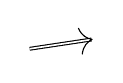
\begin{tikzpicture}\draw[->,double] (0,0)--(0.8,0.12);\end{tikzpicture}}}}

\uline{Scholie} Par les bijections (34) (38), on transporte sur
$\LMsourceMark{M000955}{\unsure{g}}_{\rho,\sigma},\ S_0g_{\rho,\sigma}$ les structures de groupes
naturelles de $\LMsourceMark{M000956}{\unsure{\widetilde{\Gamma}_{\rho,\sigma}}},\
\LMsourceMark{M000957}{\unsure{\Gamma^{b_0}_{\rho,\sigma}}}$.
Explicitant cette structure de groupe on trouve notamment pour $Sg_{\rho,\sigma}$
\[
\tag{\LMsourceMark{M000958}{\unsure{39|37}}}
\left\{\begin{array}{c}
(\alpha',\beta')(\alpha,\beta)=\alpha''\beta'',\quad
\text{avec }\alpha''=u'(\alpha)\alpha',\quad\beta''=u'(\beta)\beta'.\\
u'=u_{\LMsourceMark{M000959}{\unsure{\zeta|\xi}}',\eta'}:\
\diagram{\begin{tikzcd}[ampersand replacement=\&,column sep=large]
\LMsourceMark{M000960}{\unsure{\mathcal{C}}}\arrow[r] \& \LMsourceMark{M000961}{\unsure{\mathcal{C}}}
\end{tikzcd}},\quad\text{défini par }
\left\{\begin{aligned}
u(\rho)&=\LMsourceMark{M000962}{\unsure{\zeta|\xi}}\rho=\operatorname{int}(\alpha)\rho\\
u(\sigma)&=\eta\sigma=\operatorname{int}(\beta)\sigma
\end{aligned}\right.
\end{array}\right.
\]
(avec $\LMsourceMark{M000963}{\unsure{\zeta|\xi}}=\alpha\rho(\alpha)^{-1},\ \eta=\beta\sigma(\beta)^{-1}$).

Dans $\LMsourceMark{M000964}{\unsure{S_0\Gamma^{b_0}_{\rho,\sigma}}}$ on a un sous-groupe isom. à $L_0$, i.e.
\LMsourceMark{M000965}{\margin{\var{\inserted{
\[
\tag{39}
\diagram{\begin{tikzcd}[ampersand replacement=\&,column sep=large,row sep=small]
L_0\arrow[r] \& \LMsourceMark{M000966}{\unsure{S\Gamma'_{\rho,\sigma}}}\\
\LMsourceMark{M000967}{\unsure{\ell}}\arrow[r,mapsto] \& (\ell,1,1)
\end{tikzcd}}
\]
et on a suite exacte
\[
\tag{40}
\diagram{\begin{tikzcd}[ampersand replacement=\&,column sep=small]
1\arrow[r] \& L_0\arrow[r] \& \LMsourceMark{M000968}{\unsure{S\Gamma'_{\rho,\sigma}}}\arrow[r]
 \& \LMsourceMark{M000969}{\unsure{\Gamma}}_{\rho,\sigma}\arrow[r] \& 1
\end{tikzcd}}
\]
}}{\LMadded{
\[
\tag{39}
\diagram{\begin{tikzcd}[ampersand replacement=\&,column sep=large,row sep=small]
L_0\arrow[r] \& \LMsourceMark{M000970}{\unsure{S\Gamma'_{\rho,\sigma}}}\\
\LMsourceMark{M000971}{\unsure{\ell}}\arrow[r,mapsto] \& (\ell,1,1)
\end{tikzcd}}
\]
et on a suite exacte
\[
\tag{40}
\diagram{\begin{tikzcd}[ampersand replacement=\&,column sep=small]
1\arrow[r] \& L_0\arrow[r] \& \LMsourceMark{M000972}{\unsure{S\Gamma'_{\rho,\sigma}}}\arrow[r]
 \& \LMsourceMark{M000973}{\unsure{\Gamma}}_{\rho,\sigma}\arrow[r] \& 1
\end{tikzcd}}
\]
}}{insertion}{140-3-s510-I003}}}

\var{\deleted{
$\bullet$ \LMsourceMark{M000974}{\unsure{Posons maintenant}}
\[
\tag{39}
\begin{gathered}
M_{\rho,\sigma}\subset\operatorname{Aut}(\LMsourceMark{M000975}{\unsure{\mathcal{C}}})\\
\Vert\;\mathrm{dfn}\\
\left\{u\ \middle|\
\begin{array}{l}
\text{\LMsourceMark{M000976}{\unsure{a)|1°)}} }u\ \deleted{\LMsourceMark{M000977}{\unsure{qui}}}\ \text{fixe les classes de conj. de }\rho,\sigma\text{ dans }\LMsourceMark{M000978}{\unsure{\mathcal{C}}},\\
\quad\text{i.e. }\exists\alpha_0,\beta_0\in\LMsourceMark{M000979}{\unsure{\mathcal{C}}}\ \deleted{\LMsourceMark{M000980}{\unsure{\text{tels que}}}}\ \text{avec }\
u(\rho)=\operatorname{int}(\alpha_0)\rho,\quad u(\sigma)=\operatorname{int}(\beta_0)\sigma,\\
\text{\LMsourceMark{M000981}{\unsure{b)|2°)}} }u\ \text{fixe la classe de conjugaison de }L_0,\\
\quad\text{i.e. }\exists f\in\LMsourceMark{M000982}{\unsure{\mathcal{C}}}\ \text{tel que }u(L_0)=\operatorname{int}(f^{-1}).L_0,\\
\quad\text{i.e. }fu\in\operatorname{Norm}_{\operatorname{Aut}(\LMsourceMark{M000983}{\unsure{\mathcal{C}}})}(L_0)
\end{array}\right\}
\end{gathered}
\]
donc par définition de
\[
\tag{41}
\LMsourceMark{M000984}{\unsure{\mathcal{T}|\Gamma}}_{\rho,\sigma}\overset{\mathrm{dfn}}{=}
Z_\rho\mathbin{\times}_{\Gamma_{\rho,\sigma}}Z_\sigma
\]
donc
\[
\tag{42}
\diagram{\begin{tikzcd}[ampersand replacement=\&,column sep=small]
1\arrow[r] \& SZ_\rho\times SZ_\sigma\arrow[r]
 \& \LMsourceMark{M000985}{\unsure{\mathcal{T}|\Gamma}}_{\rho,\sigma}\arrow[r,"\LMsourceMark{M000986}{\unsure{\delta_{\mathcal{T}}}}"]
 \& \Gamma_{\rho,\sigma}\arrow[r] \& 1
\end{tikzcd}}
\]
}}{\LMsourceMark{M000987}{\LMcancelledDoubts{\LMsourceMark{M000988}{\unsure{Posons maintenant}}\quad \(\LMsourceMark{M000989}{\unsure{\mathcal{C}}}\)\quad \LMsourceMark{M000990}{\unsure{a)|1°)}}\quad \(\LMsourceMark{M000991}{\unsure{qui}}\)\quad \(\LMsourceMark{M000992}{\unsure{\mathcal{C}}}\)\quad \(\LMsourceMark{M000993}{\unsure{\mathcal{C}}}\)\quad \(\LMsourceMark{M000994}{\unsure{\text{tels que}}}\)\quad \LMsourceMark{M000995}{\unsure{b)|2°)}}\quad \(\LMsourceMark{M000996}{\unsure{\mathcal{C}}}\)\quad \(\LMsourceMark{M000997}{\unsure{\mathcal{C}}}\)\quad \(\LMsourceMark{M000998}{\unsure{\mathcal{T}|\Gamma}}\)\quad \(\LMsourceMark{M000999}{\unsure{\mathcal{T}|\Gamma}}\)\quad \(\LMsourceMark{M001000}{\unsure{\delta_{\mathcal{T}}}}\)}}}{deletion}{140-3-s510-D005}
\LMsourceMark{M001001}{\mspage{509}}

\LMflushnotes\LMflushpages
\ifnum\LMform=1
\begin{LMapparatus}
\LMentry{140-3-s510-D001}{suppression}{\(\deleted{\LMsourceMark{M001002}{\unsure{S\widetilde{\Gamma}^{0}_{\rho,\sigma}}}\LMsourceMark{M001003}{\unsure{=\widetilde M_{\rho,\sigma}^{0}}}\LMsourceMark{M001004}{\unsure{\subset S_0\Gamma_{\rho,\sigma}}}}\)
}{\emph{\LMomittedlabel}}{Passage biffé dans le manuscrit : la suppression suit l'état final de l'auteur; les doutes de lecture restent signalés.}{}
\LMentry{140-3-s510-I001}{insertion}{\(\inserted{\LMsourceMark{M001005}{\unsure{S_0\Gamma^{b_0}_{\rho,\sigma}}}}\)
}{\emph{\LMinsertedlabel}}{Ajout explicite de l'auteur : intégré à l'endroit indiqué par la transcription, sans modifier sa lecture.}{}
\LMentry{140-3-s510-D002}{suppression}{\deleted{i.e. $\LMsourceMark{M001006}{\unsure{S\Gamma'_{\rho,\sigma}}}$}
}{\emph{\LMomittedlabel}}{Passage biffé dans le manuscrit : la suppression suit l'état final de l'auteur; les doutes de lecture restent signalés.}{}
\LMentry{140-3-s510-D003}{suppression}{\deleted{\LMsourceMark{M001007}{\unsure{ici}}}
}{\emph{\LMomittedlabel}}{Passage biffé dans le manuscrit : la suppression suit l'état final de l'auteur; les doutes de lecture restent signalés.}{}
\LMentry{140-3-s510-D004}{suppression}{\(\deleted{\LMsourceMark{M001008}{\unsure{(ua^{-1},ub^{-1})}}}\)
}{\emph{\LMomittedlabel}}{Passage biffé dans le manuscrit : la suppression suit l'état final de l'auteur; les doutes de lecture restent signalés.}{}
\LMentry{140-3-s510-I002}{insertion}{\(\inserted{(\LMsourceMark{M001009}{\unsure{\zeta|\xi}},\eta)}\)
}{\emph{\LMinsertedlabel}}{Ajout explicite de l'auteur : intégré à l'endroit indiqué par la transcription, sans modifier sa lecture.}{}
\LMentry{140-3-s510-I003}{insertion}{\inserted{
\[
\tag{39}
\diagram{\begin{tikzcd}[ampersand replacement=\&,column sep=large,row sep=small]
L_0\arrow[r] \& \LMsourceMark{M001010}{\unsure{S\Gamma'_{\rho,\sigma}}}\\
\LMsourceMark{M001011}{\unsure{\ell}}\arrow[r,mapsto] \& (\ell,1,1)
\end{tikzcd}}
\]
et on a suite exacte
\[
\tag{40}
\diagram{\begin{tikzcd}[ampersand replacement=\&,column sep=small]
1\arrow[r] \& L_0\arrow[r] \& \LMsourceMark{M001012}{\unsure{S\Gamma'_{\rho,\sigma}}}\arrow[r]
 \& \LMsourceMark{M001013}{\unsure{\Gamma}}_{\rho,\sigma}\arrow[r] \& 1
\end{tikzcd}}
\]
}
}{\emph{\LMinsertedlabel}}{Ajout explicite de l'auteur : intégré à l'endroit indiqué par la transcription, sans modifier sa lecture.}{}
\LMentry{140-3-s510-D005}{suppression}{\deleted{
$\bullet$ \LMsourceMark{M001014}{\unsure{Posons maintenant}}
\[
\tag{39}
\begin{gathered}
M_{\rho,\sigma}\subset\operatorname{Aut}(\LMsourceMark{M001015}{\unsure{\mathcal{C}}})\\
\Vert\;\mathrm{dfn}\\
\left\{u\ \middle|\
\begin{array}{l}
\text{\LMsourceMark{M001016}{\unsure{a)|1°)}} }u\ \deleted{\LMsourceMark{M001017}{\unsure{qui}}}\ \text{fixe les classes de conj. de }\rho,\sigma\text{ dans }\LMsourceMark{M001018}{\unsure{\mathcal{C}}},\\
\quad\text{i.e. }\exists\alpha_0,\beta_0\in\LMsourceMark{M001019}{\unsure{\mathcal{C}}}\ \deleted{\LMsourceMark{M001020}{\unsure{\text{tels que}}}}\ \text{avec }\
u(\rho)=\operatorname{int}(\alpha_0)\rho,\quad u(\sigma)=\operatorname{int}(\beta_0)\sigma,\\
\text{\LMsourceMark{M001021}{\unsure{b)|2°)}} }u\ \text{fixe la classe de conjugaison de }L_0,\\
\quad\text{i.e. }\exists f\in\LMsourceMark{M001022}{\unsure{\mathcal{C}}}\ \text{tel que }u(L_0)=\operatorname{int}(f^{-1}).L_0,\\
\quad\text{i.e. }fu\in\operatorname{Norm}_{\operatorname{Aut}(\LMsourceMark{M001023}{\unsure{\mathcal{C}}})}(L_0)
\end{array}\right\}
\end{gathered}
\]
donc par définition de
\[
\tag{41}
\LMsourceMark{M001024}{\unsure{\mathcal{T}|\Gamma}}_{\rho,\sigma}\overset{\mathrm{dfn}}{=}
Z_\rho\mathbin{\times}_{\Gamma_{\rho,\sigma}}Z_\sigma
\]
donc
\[
\tag{42}
\diagram{\begin{tikzcd}[ampersand replacement=\&,column sep=small]
1\arrow[r] \& SZ_\rho\times SZ_\sigma\arrow[r]
 \& \LMsourceMark{M001025}{\unsure{\mathcal{T}|\Gamma}}_{\rho,\sigma}\arrow[r,"\LMsourceMark{M001026}{\unsure{\delta_{\mathcal{T}}}}"]
 \& \Gamma_{\rho,\sigma}\arrow[r] \& 1
\end{tikzcd}}
\]
}
}{\emph{\LMomittedlabel}}{Passage biffé dans le manuscrit : la suppression suit l'état final de l'auteur; les doutes de lecture restent signalés.}{}
\end{LMapparatus}
\fi
\ifnum\LMform=2
\par\smallskip\begingroup\footnotesize\noindent\textcolor{gray}{\rule{.2\linewidth}{.35pt}}\par
\noindent\textit{\LMdoubtheading.}\par
\LMcarryover{140-3-s510-D001}{\(\LMsourceMark{M001027}{\unsure{S\widetilde{\Gamma}^{0}_{\rho,\sigma}}}\)\quad \(\LMsourceMark{M001028}{\unsure{=\widetilde M_{\rho,\sigma}^{0}}}\)\quad \(\LMsourceMark{M001029}{\unsure{\subset S_0\Gamma_{\rho,\sigma}}}\)
}
\LMcarryover{140-3-s510-D002}{\(\LMsourceMark{M001030}{\unsure{S\Gamma'_{\rho,\sigma}}}\)
}
\LMcarryover{140-3-s510-D003}{\LMsourceMark{M001031}{\unsure{ici}}
}
\LMcarryover{140-3-s510-D004}{\(\LMsourceMark{M001032}{\unsure{(ua^{-1},ub^{-1})}}\)
}
\LMcarryover{140-3-s510-D005}{\LMsourceMark{M001033}{\unsure{Posons maintenant}}\quad \(\LMsourceMark{M001034}{\unsure{\mathcal{C}}}\)\quad \LMsourceMark{M001035}{\unsure{a)|1°)}}\quad \(\LMsourceMark{M001036}{\unsure{qui}}\)\quad \(\LMsourceMark{M001037}{\unsure{\mathcal{C}}}\)\quad \(\LMsourceMark{M001038}{\unsure{\mathcal{C}}}\)\quad \(\LMsourceMark{M001039}{\unsure{\text{tels que}}}\)\quad \LMsourceMark{M001040}{\unsure{b)|2°)}}\quad \(\LMsourceMark{M001041}{\unsure{\mathcal{C}}}\)\quad \(\LMsourceMark{M001042}{\unsure{\mathcal{C}}}\)\quad \(\LMsourceMark{M001043}{\unsure{\mathcal{T}|\Gamma}}\)\quad \(\LMsourceMark{M001044}{\unsure{\mathcal{T}|\Gamma}}\)\quad \(\LMsourceMark{M001045}{\unsure{\delta_{\mathcal{T}}}}\)
}
\par\endgroup\smallskip
\fi

% END PACKAGE LM_C3-492-510
\end{document}
